% A LaTeX template for MSc Thesis submissions to 
% Politecnico di Milano (PoliMi) - School of Industrial and Information Engineering
%
% S. Bonetti, A. Gruttadauria, G. Mescolini, A. Zingaro
% e-mail: template-tesi-ingind@polimi.it
%
% Last Revision: October 2021
%
% Copyright 2021 Politecnico di Milano, Italy. NC-BY

\documentclass{Configuration_Files/PoliMi3i_thesis}

%------------------------------------------------------------------------------
%	REQUIRED PACKAGES AND  CONFIGURATIONS
%------------------------------------------------------------------------------

% CONFIGURATIONS
\usepackage{parskip} % For paragraph layout
\usepackage{setspace} % For using single or double spacing
\usepackage{emptypage} % To insert empty pages
\usepackage{multicol} % To write in multiple columns (executive summary)
\setlength\columnsep{15pt} % Column separation in executive summary
\setlength\parindent{0pt} % Indentation
\raggedbottom  

% PACKAGES FOR TITLES
\usepackage{titlesec}
% \titlespacing{\section}{left spacing}{before spacing}{after spacing}
\titlespacing{\section}{0pt}{3.3ex}{2ex}
\titlespacing{\subsection}{0pt}{3.3ex}{1.65ex}
\titlespacing{\subsubsection}{0pt}{3.3ex}{1ex}
\usepackage{color}

% PACKAGES FOR LANGUAGE AND FONT
\usepackage[english]{babel} % The document is in English  
\usepackage[utf8]{inputenc} % UTF8 encoding
\usepackage[T1]{fontenc} % Font encoding
\usepackage[11pt]{moresize} % Big fonts

% PACKAGES FOR IMAGES
\usepackage{graphicx}
\usepackage{transparent} % Enables transparent images
\usepackage{eso-pic} % For the background picture on the title page
\usepackage{subfig} % Numbered and caption subfigures using \subfloat.
\usepackage[export]{adjustbox}
\usepackage{tikz} % A package for high-quality hand-made figures.
\usetikzlibrary{}
\graphicspath{{./Images/}} % Directory of the images
\usepackage{caption} % Coloured captions
\usepackage{xcolor} % Coloured captions
\usepackage{amsthm,thmtools,xcolor} % Coloured "Theorem"
\usepackage{float}
\usepackage{placeins}

% STANDARD MATH PACKAGES
\usepackage{amsmath}
\usepackage{amsthm}
\usepackage{amssymb}
\usepackage{amsfonts}
\usepackage{bm}
\usepackage[overload]{empheq} % For braced-style systems of equations.
\usepackage{fix-cm} % To override original LaTeX restrictions on sizes

% PACKAGES FOR TABLES
\usepackage{tabularx}
\usepackage{longtable} % Tables that can span several pages
\usepackage{colortbl}

% PACKAGES FOR ALGORITHMS (PSEUDO-CODE)
\usepackage{algorithm}
\usepackage{algorithmic}

% PACKAGES FOR REFERENCES & BIBLIOGRAPHY
\usepackage[colorlinks=true,linkcolor=black,anchorcolor=black,citecolor=black,filecolor=black,menucolor=black,runcolor=black,urlcolor=black]{hyperref} % Adds clickable links at references
\usepackage{cleveref}
\usepackage[square, numbers, sort&compress]{natbib} % Square brackets, citing references with numbers, citations sorted by appearance in the text and compressed
\bibliographystyle{abbrvnat} % You may use a different style adapted to your field

% OTHER PACKAGES
\usepackage{pdfpages} % To include a pdf file
\usepackage{afterpage}
\usepackage{lipsum} % DUMMY PACKAGE
\usepackage{fancyhdr} % For the headers
\usepackage[export]{adjustbox}
\fancyhf{}

% Input of configuration file. Do not change config.tex file unless you really know what you are doing. 
% Configuration package
\usepackage[bottom=2.0cm,top=2.0cm,left=2.0cm,right=2.0cm]{geometry}
\raggedbottom 

% Create color bluePoli (-> manuale grafica coordinata:  https://www.polimi.it/fileadmin/user_upload/il_Politecnico/grafica-coordinata/2015_05_11_46xy_manuale_grafica_coordinata.pdf)
\definecolor{bluePoli}{cmyk}{0.4,0.1,0,0.4}

% Custom theorem environments
\declaretheoremstyle[
  headfont=\color{bluePoli}\normalfont\bfseries,
  bodyfont=\color{black}\normalfont\itshape,
]{colored}

\captionsetup[figure]{labelfont={color=bluePoli}} % Set colour of the captions
\captionsetup[table]{labelfont={color=bluePoli}} % Set colour of the captions
\captionsetup[algorithm]{labelfont={color=bluePoli}} % Set colour of the captions

\theoremstyle{colored}
\newtheorem{theorem}{Theorem}[section]
\newtheorem{proposition}{Proposition}[section]

% Enhances the features of the standard "table" and "tabular" environments.
\newcommand\T{\rule{0pt}{2.6ex}}
\newcommand\B{\rule[-1.2ex]{0pt}{0pt}}

% Algorithm description
\newcounter{algsubstate}
\renewcommand{\thealgsubstate}{\alph{algsubstate}}
\newenvironment{algsubstates}{
    \setcounter{algsubstate}{0}%
    \renewcommand{\STATE}{%
    \stepcounter{algsubstate}%
    \Statex {\small\thealgsubstate:}\space}
    }{}
    
% Custom theorem environment
\newcolumntype{L}[1]{>{\raggedright\let\newline\\\arraybackslash\hspace{0pt}}m{#1}}
\newcolumntype{C}[1]{>{\centering\let\newline\\\arraybackslash\hspace{0pt}}m{#1}}
\newcolumntype{R}[1]{>{\raggedleft\let\newline\\\arraybackslash\hspace{0pt}}m{#1}}

% Custom itemize environment
\setlist[itemize,1]{label=$\bullet$}
\setlist[itemize,2]{label=$\circ$}
\setlist[itemize,3]{label=$-$}
\setlist{nosep}

% Create command for background pic
\newcommand\BackgroundPic{% Adding background picture
	\put(237,365){
	    \parbox[b][\paperheight]{\paperwidth}{%
	    \vfill
		\centering
		\transparent{0.4}
		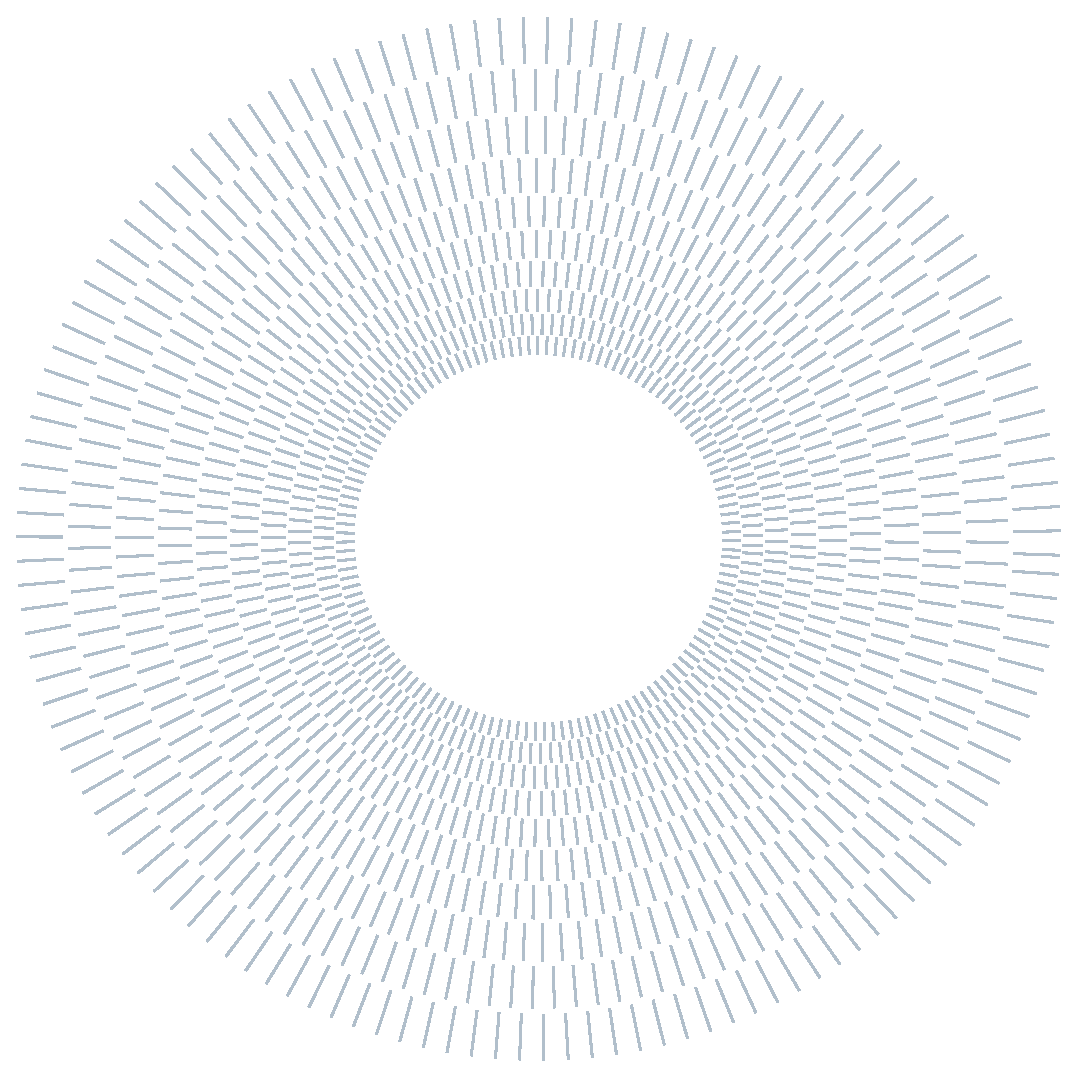
\includegraphics[width=0.44\paperwidth]{raggiera_polimi.eps}%
		\vfill}
		}
}

% Set indentation
\setlength\parindent{0pt}

% Custom title commands
\titleformat{\section}
{\color{bluePoli}\normalfont\Large\bfseries}
{\color{bluePoli}\thesection.}{1em}{}
\titlespacing*{\section}
{0pt}{3.3ex}{3.3ex}

\titleformat{\subsection}
{\color{bluePoli}\normalfont\large\bfseries}
{\color{bluePoli}\thesubsection.}{1em}{}
\titlespacing*{\subsection}
{0pt}{3.3ex}{3.3ex}

% Custom headers and footers
\pagestyle{fancy}
\fancyhf{}
      
\fancyfoot{}
\fancyfoot[C]{\thepage} % page
\renewcommand{\headrulewidth}{0mm} % headrule width
\renewcommand{\footrulewidth}{0mm} % footrule width

\makeatletter
\patchcmd{\headrule}{\hrule}{\color{black}\hrule}{}{} % headrule
\patchcmd{\footrule}{\hrule}{\color{black}\hrule}{}{} % footrule
\makeatother

%----------------------------------------------------------------------------
%	NEW COMMANDS DEFINED
%----------------------------------------------------------------------------

% EXAMPLES OF NEW COMMANDS
\newcommand{\bea}{\begin{eqnarray}} % Shortcut for equation arrays
\newcommand{\eea}{\end{eqnarray}}
\newcommand{\e}[1]{\times 10^{#1}}  % Powers of 10 notation

%----------------------------------------------------------------------------
%	ADD YOUR PACKAGES (be careful of package interaction)
%----------------------------------------------------------------------------

%----------------------------------------------------------------------------
%	ADD YOUR DEFINITIONS AND COMMANDS (be careful of existing commands)
%----------------------------------------------------------------------------
\Urlmuskip=0mu  plus 10mu
%----------------------------------------------------------------------------
%	BEGIN OF YOUR DOCUMENT
%----------------------------------------------------------------------------

\begin{document}

\fancypagestyle{plain}{%
\fancyhf{} % Clear all header and footer fields
\fancyhead[RO,RE]{\thepage} %RO=right odd, RE=right even
\renewcommand{\headrulewidth}{0pt}
\renewcommand{\footrulewidth}{0pt}}
\interfootnotelinepenalty=10000
%----------------------------------------------------------------------------
%	TITLE PAGE
%----------------------------------------------------------------------------

\pagestyle{empty} % No page numbers
\frontmatter % Use roman page numbering style (i, ii, iii, iv...) for the preamble pages

\puttitle{
	title=Quality Diversity in Procedural Generation of First Person Shooter Maps, % Title of the thesis
	name=Simone de Donato, % Author Name and Surname
	course=Computer Science and Engineering - Ingegneria Informatica, % Study Programme (in Italian)
	ID  = 223220,  % Student ID number (numero di matricola)
	advisor= Prof. Pierluca Lanzi, % Supervisor name
	coadvisor=Prof. Daniele Loiacono, % Co-Supervisor name, remove this line if there is none
	academicyear={2023-24},  % Academic Year
} % These info will be put into your Title page 

%----------------------------------------------------------------------------
%	PREAMBLE PAGES: ABSTRACT (inglese e italiano), EXECUTIVE SUMMARY
%----------------------------------------------------------------------------
\startpreamble
\setcounter{page}{1} % Set page counter to 1

% ABSTRACT IN ENGLISH
\chapter*{Abstract} 
\textit{Quality Diversity} algorithms are a relatively recent type of \textit{evolutionary algorithm} which takes inspiration from the process of biological evolution to generate a set of solutions which are not only trying to optimize for a certain objective, but that are also diverse and novel. These algorithms, such as MAP-Elites, have seen widespread use in many scientific fields, and have been used in the literature for \textit{Procedural Content Generation} in various games, including platformers, puzzle games and card games.

Many commercial games have utilized \textit{Procedural Content Generation} to great success, yet competitive First-Person Shooters, despite being among the most popular games in the industry, rarely utilize it in any capacity, let alone for the generation of maps, which could decrease the time spent on the hard and time-consuming task of \textit{level design}, that otherwise relies mostly on talent and experience.

Scientific studies have recently started to explore the use of \textit{evolutionary algorithms} for the generation of maps for FPS games, but have yet to use \textit{Quality Diversity} algorithms, which are particularly suited for the task, given their focus on both diversity and quality.

In this work we aim to fill this gap by using \textit{MAP-Elites with Sliding Boundaries} (MESB) to generate maps for Project Arena, a research-oriented Unity framework for First-Person Shooters. We will define two new map representations (\textit{Point-Line} and \textit{SMT-Genome}) and extract metrics that describe each map, study the correlation between these metrics and use some of them to search for diverse and high-quality maps using \textit{MESB}.

Results show that \textit{Quality Diversity} algorithms can be successfully used for this purpose, and we compared the performance of our new representations with two existing ones, \textit{All-Black} and \textit{Grid-Graph}, showing that the new representations can generate maps with higher diversity and overall quality, suggesting that the representation used for the generation of maps is a key factor.


\textbf{Keywords:} Quality Diversity, Procedural Content Generation, FPS, MAP-Elites, level design % Keywords

% ABSTRACT IN ITALIAN
\chapter*{Abstract in lingua italiana}
Gli algoritmi di \textit{Quality Diversity} sono una categoria di \textit{algoritmi evolutivi} relativamente recente che si ispira al processo dell'evoluzione biologica per generare un insieme di soluzioni che siano ottimali rispetto ad un obiettivo, ma che allo stesso tempo siano anche varie.
Tali algoritmi, quale MAP-Elites, sono stati utilizzati in molti campi scientifici, tra i quali spicca per interesse la \textit{Genrazione Procedurale di Contenuti} nei giochi, tra cui si annoverano ad esempio platformer, giochi puzzle e giochi di carte.

Molti giochi hanno utilizzato la \textit{Generazione Procedurale di Contenuti} con successo, tuttavia gli Sparatutto in Prima Persona competitivi, nonostante siano tra i più popolari del settore, raramente la utilizzano, tantomeno al fine di generare mappe di gioco, quando questa tecnica potrebbe ridurre il tempo speso per il dispendioso compito di \textit{level design}, il quale altrimenti si basa sul talento e sull'esperienza individuale.

Di recente, diversi studi hanno utilizzato \textit{algoritmi evolutivi} per la generazione di mappe per giochi FPS, ma ancora non sono stati utilizzati algoritmi di \textit{Quality Diversity}, i quali sono particolarmente indicati dato il loro focus sia sulla diversità che sulla qualità.

In questa tesi ci proponiamo di colmare questa lacuna utilizzando \textit{MAP-Elites with Sliding Boundaries} (MESB) per generare mappe per Project Arena, un framework sviluppato in Unity orientato alla ricerca per i First-Person Shooters. Definiremo due nuove rappresentazioni per le mappe (\textit{Point-Line} e \textit{SMT-Genome}) ed estrarremo metriche che descrivono ciascuna mappa, studieremo la correlazione tra queste metriche e ne utilizzaremo alcune per evolvere mappe che siano varie e di alta qualità utilizzando \textit{MESB}.

I risultati mostrano che gli algoritmi di \textit{Quality Diversity} possono essere utilizzati con successo per questo scopo, e abbiamo confrontato le prestazioni delle nostre nuove rappresentazioni con due esistenti, \textit{All-Black} e \textit{Grid-Graph}, mostrando che le nuove rappresentazioni generano mappe con maggiore diversità e qualità complessiva, suggerendo che la rappresentazione scelta per la generazione di mappe è un fattore chiave.



\textbf{Parole chiave:} Quality Diversity, Generazione Procedurale di Contenuti, FPS, MAP-Elites, level design % Keywords (italian)

%----------------------------------------------------------------------------
%	LIST OF CONTENTS/FIGURES/TABLES/SYMBOLS
%----------------------------------------------------------------------------

% TABLE OF CONTENTS
\thispagestyle{empty}
\tableofcontents % Table of contents 
\thispagestyle{empty}
\cleardoublepage

%-------------------------------------------------------------------------
%	THESIS MAIN TEXT
%-------------------------------------------------------------------------
% In the main text of your thesis you can write the chapters in two different ways:
%
%(1) As presented in this template you can write:
%    \chapter{Title of the chapter}
%    *body of the chapter*
%
%(2) You can write your chapter in a separated .tex file and then include it in the main file with the following command:
%    \chapter{Title of the chapter}
%    \input{chapter_file.tex}
%
% Especially for long thesis, we recommend you the second option.

\addtocontents{toc}{\vspace{2em}} % Add a gap in the Contents, for aesthetics
\mainmatter % Begin numeric (1,2,3...) page numbering

% --------------------------------------------------------------------------
% NUMBERED CHAPTERS % Regular chapters following
% --------------------------------------------------------------------------
\chapter{Introduction}
\label{ch:introduction}

It is widely agreed that, among the many elements that make a game enjoyable, \textit{level design} is one of the most important. \textit{Level design} refers to the process of designing and creating the worlds and environments where the player interacts and plays. Despite its importance, \textit{level design} is a complex and time-consuming task, which requires extensive knowledge and experience. 

In order to create engaging experiences for players games may require a lot of content to be designed and created, which can be a time-consuming and expensive process. In order to create games with more content and that offer more replayability, the industry has seen the rise of \textit{Procedural Content Generation} (PCG) techniques, which refer to the class of algorithms and methods used to generate content automatically. Critically acclaimed games that range from indies, such as \textit{Minecraft}, to AAA titles, such as \textit{No Man's Sky}, employ PCG techniques to various degrees to offer ever-changing gameplay. 

One relevant question in the context of PCG is how to generate content that is not only of high quality, but also novel and diverse. \textit{Quality Diversity} optimization refers to a relatively new class of algorithms that, taking inspiration from the process of biological evolution, aims to answer this very question by generating a diverse set of high-quality solutions, instead of a single one. In the literature, \textit{Quality Diversity} algorithms have been used to generate content for different genres, such as platformers and puzzle games.

\textit{First-Person Shooters} (FPS), especially multiplayer competitive ones, are among the most popular games in the industry. Despite this, the topic of level design for FPS has seen only a few scientific works which have tried to define patterns and techniques, but ultimately still lacks specific standards. Moreover, PCG has yet to be used in a critically acclaimed competitive FPS, despite having shown great potential through its application in other genres. Contrary to the industry, scientific studies have taken an increasing interest in the use of PCG in FPS, with \textit{evolutionary algorithms} being used to generate maps. However, despite being particularly suited for PCG, given their focus on both diversity and quality, \textit{Quality Diversity} algorithms have yet to be applied to FPS games.

Our aim with this thesis is that of filling this gap by exploring the use of a Quality Diversity algorithm, \textit{MAP-Elites with Sliding Boundaries} (MESB) \cite{fontaine_mapping_2019}, to the generation of maps for multiplayer competitive FPS games. We will define ways to represent maps and extract metrics that describe each map, study the correlation between these metrics and use them to search for diverse and high-quality maps using \textit{MESB}. We will compare the performance of different representations and discuss the results obtained.

\section{Contents of the thesis}
We structure our thesis as follows:

In the second chapter we will explore the state of the art regarding the main concepts of interests in our work, which include \textit{level design} for FPS games, the \textit{balancing} of competitive multiplayer games and the use of Procedural Content Generation (PCG) in games. We will particularly examine \textit{search-based} PCG, which will allow us to understand how PCG has been applied to the generation of FPS maps in the literature. Finally, we will introduce the concept of \textit{Quality Diversity} along with how it has been used for the generation of content in games.

In the third chapter we will present the frameworks we have used to conduct our research: \textit{Project Arena}, a research-oriented framework for FPS games developed in Unity by \citet{ballabio_online_2018}, and \textit{pyribs} \cite{tjanaka_pyribs_2023}, a Python library for Quality Diversity algorithms. We will explain the reason for our choices along with a description of their capabilities and structure. 

In the fourth chapter we will first describe the genome representations used to describe and evolve maps. We will present All-Black \cite{cardamone_evolving_2011} and Grid-Graph \cite{bari_evolutionary-based_2023}, which have already been used to evolve maps with evolutionary algorithms, and introduce our own representations, which we called \textit{Point-Line} and \textit{SMT-Genome}. Then, we will discuss the features we have extracted from each map, categorizing them in \textit{emergent}, which are directly extracted from simulated gameplay, and \textit{topological}, which are extracted from the map's structure.

In the fifth chapter we will present the experiments we have conducted. First, we are going to make sure that the emergent features chosen are not noisy, making them suitable to describe maps. Then we will analyze the correlation between different features to establish patterns and groups of features. Following, we will select relevant features to illuminate leveraging the result of running the \textit{t-SNE} on different high-dimensional spaces that describe the maps. Finally, we establish three \textit{behavioral characterizations} and run the \textit{MAP-Elites with Sliding Boundaries} algorithm, analyze the results and compare the performance of the different representations.

Finally, we sum up the work done, discuss the results, argue possible shortcomings of our work and propose prospects for future work.


\chapter{State of the art}
\label{ch:state_of_the_art}
In the following chapter we are first going to examine level design from an historical and industry perspective, with a particular focus on First-Person Shooter (FPS) games and academic research on the topic of level design for FPS games.

Then we are going to look at how balancing is defined and what elements of multiplayer games make a game balanced. Specifically, we are also going to examine how maps influence the balance of FPS games.

We will also review the history of commercial games utilizing Procedural Content Generation (PCG) and provide a taxonomy of the approaches used, including an examination of Search-Based PCG. Furthermore, we will analyze the state of the art in academic research on PCG for maps in FPS games.

Finally, we will look into Quality Diversity methods, specifically at MAP-Elites, and present how it has been used in the literature to generate videogame content.

\section{Level design in First-Person Shooter games}
\label{sec:level_design}
In the field of game design and development, level design can be defined as the discipline of crafting video game levels, places and missions to achieve gameplay that is both fun and balanced, leveraging genre and game-specific mechanics.

In the early days of video game development, game programmers also doubled as level designers, but as the industry grew bigger the importance of a dedicated level designer role became apparent. Level design is arguably the biggest factor in ensuring that the player is always engaged and that the gameplay mechanics are fully utilized. Despite this, level design, as a discipline, doesn't yet have clearly defined processes and terminology and instead relies on the talent and experience of talented individuals.

A number of books have been written on the topic, most of which discuss common practices and describe the tools used by level designers, but don't detail how level design creates gameplay. As an example, in his book \textit{Level Design for Games: Creating Compelling Game Experiences}, \Citeauthor{co_level_2006} explains the process of designing a level for an FPS game in practical detail, starting from a brainstorming phase, through building the level in Unreal Engine\footnote{Game engine developed by Epic Games.}, and to finally testing and improving the level \cite{co_level_2006}, but does not delve in how this process creates gameplay. \cite{hullett_design_2010}

Shorter academic works have focused on certain aspects of level design which are independent of genre: some have focused on gameplay idioms such as correctly pacing the level, creating tension and creating a suitable level of challenge, while others focused on spatial characteristics of the playing environment, such as the spatial configurations or how the player navigates the level. \cite{hullett_design_2010}

In First-Person Shooters (FPS)\footnote{First-Person Shooters are a genre of video games that are played from the perspective of the player character and that revolve around gun-fighting, such as \textit{Wolfenstein 3D} (id Software, 1992), \textit{Doom} (id Software, 1993) and \textit{Quake} (id Software, 1996).} level design takes the form of designing the level or map that the player is placed in, minding the placement of objects, covers and enemies. There exist many kinds of FPS games, each with different gameplay mechanics (e.g. \textit{Titanfall}\footnote{Respawn Entertainment, 2014}, which allows the player to run on walls) and level design principles. 

The most important distinction that can be drawn is between singleplayer and multiplayer FPS games. Singleplayer games usually see the player traversing a level in linear fashion, completing objectives defined by the game designer, such as solving puzzles or defeating enemies, and optionally discovering secrets or uncovering a story, such as in \textit{Half-Life}\footnote{Valve Corporation, 1998}. In multiplayer games like \textit{Call of Duty}\footnote{Infinity Ward, 2003} players compete to achieve a goal before their opponent (e.g. capture the flag, kill the enemy team) and the levels are designed to facilitate and balance this competition. Other multiplayer games may instead require players to cooperate to reach a common goal, such as in \textit{Left 4 Dead}\footnote{Valve Corporation, 2008}, where players have to survive a zombie apocalypse together or in \textit{Portal 2}\footnote{Valve Software, 2011}, where players have to solve puzzles together.

The differences between these types of games are reflected in the level design principles that are used. While singleplayer and cooperative games may thrive from having maps that put the player in a position of disadvantage to increase challenge and tension, competitive multiplayer games require maps that are balanced and fair to all players. 

Given that FPS games usually also present multiple game modes that naturally require diverse level designs, academic research has either focused on a singular and more universal aspect (such as pace, challenge or tension), or has tried to analyze a specific game (or type of game) to examine a specific feature of its level design.


\Citeauthor*{guttler_spatial_2003} outlined the basic spatial principles of level design in multiplayer First-Person Shooters with special reference to \textit{Counter-Strike} \cite{guttler_spatial_2003}. They argue  that successful level design for multiplayer FPS is based on several factors, such as gameplay, theme, architecture and spatial structure, and that the level designer will greatly benefit from leveraging theoretical tools to develop maps, as such tools would make  eliciting specific gameplay during game sessions easier. By analyzing the gameplay of existing maps and their layouts they deduce the basic spatial principles of \textit{Counter-Strike}'s level design and elaborate on how to best apply them to create a successful map. 

\Citeauthor{larsen_level_2006} argues the usefulness of patterns in fields ranging from software development to film making, and proposes that they can be used to describe level design practices in the domain of FPS games. He specifically focuses on several competitive multiplayer FPS games (\textit{Unreal Tournament 2004}\footnote{Epic Games, 2004}, \textit{Day of Defeat: Source}\footnote{Valve Corporation, 2005} and \textit{Battlefield 1942}\footnote{DICE, 2002}) and extracts common design patterns by analyzing several levels in search of common ways of solving problematic elements. He defines the patterns of "multiple paths", "local fights", "collision points", "reference points", "defense areas" and "risk incentive". For each identified pattern, he provides a description, examples on how to use the pattern, consequences on gameplay, how it interacts with other patterns and commercial examples of its use. He concludes that recurring patterns should not streamline levels but instead be used as tools to design better levels. \cite{larsen_level_2006}

In a similar vein, \Citeauthor*{hullett_design_2010} adapt how patterns are characterized in the field of software engineering to the domain of single player FPS level design. They use this characterization to identify a set of design patterns commonly used in FPS level design, which can be used as a language for describing design practices in the domain of FPS games. Patterns are divided into "patterns for positional advantage" (sniper locations, gallery, choke point), "patterns for large scale combat" (arena, stronghold), "patterns for alternate gameplay" (turret, vehicle selection) and "pattern for alternate routes" (split-level, hidden area, flanking route). For each, they provide a description, how it can be modified, the gameplay it creates, how it interacts with other patterns and commercial examples of its use. 
They argue that patterns can help designers generate new ideas by combining them, and can also help solve design problems by providing guidance on what to add or remove to achieve a gameplay goal, since patterns offer a clear cause-effect explanation. They also argue that these patterns can be generalized and reasonably applied to multiplayer games in some situations. \cite{hullett_design_2010}

\section{Balance in competitive multiplayer video games}
\label{sec:balance}
A concept that is closely related to level design is \textit{game balance}. Giving a general definition for "game balance" is a harder task than it might seem, as \citeauthor{becker_what_2020} note in their semantic analysis based on other publications on the theme of balancing games of various kinds. They conclude that further research would be needed to reach a commonly agreeable definition, given that the authors they analyzed did not have a common central goal, with some focusing on the end goal of "fun", other on "challenge" and others on "flow". \cite{becker_what_2020}

For multiplayer games specifically, \citeauthor{sirlin_balancing_2014} states that a game is balanced if the player can choose between a sufficiently large array of options which are viable, meaning that they are different, meaningful and not dominated by other options. These choices can be made before the game starts (fairness) or during the game itself (viable options). \cite{sirlin_balancing_2014}

When players can choose between different sets of options before starting the game we talk about \textit{asymmetric games} (e.g. most FPS games where you can select your weapon, or fighting games with multiple playable characters), while in \textit{symmetric games} players start the game with an identical and static set of options (e.g. games like Tetris\footnote{Aleksej Pažitnov, Vadim Gerasimov, Dmitrij Pavlovskij, 1984}, where players are fed the same pieces during the competition) \cite{sirlin_balancing_2014}. The former are naturally easy to balance, but often games introduce options to stand out and make the game more replayable, deep and fun; a fighting game with only a single character would surely be balanced, but also boring. 

A concept that \citeauthor{sirlin_balancing_2014} highlights is that of "dominant strategies". For a competitive game to be balanced a player should be able to choose at any time between many viable options, but if one of those is too strong it would both make other options meaningless and reduce the strategic value of the game. To allow for a balanced game with deep strategy it can be beneficial to consider the concept of "Yomi"\footnote{A Japanese word that can be translated to "Reading". In this context, it is meant as "reading the mind of your opponent".}, which refers to the fact that if a player were to read the opponent's mind, he should then be able to counter the opponent's strategy. A dominant strategy is one so strong that counters may not exist. \cite{sirlin_balancing_2014}

When strictly considering asymmetric games, authors agree that balancing should not be the sole goal \cite{sirlin_balancing_2014} \cite{portwnow_perfect_2012} \cite{brown_how_2019}. These games are designed to allow players to employ various strategies and tactics, so while no one strategy should be strictly better than others, if all strategies were instead perfectly balanced the game may provide un-fun options that feel very similar to each other \cite{sakurai_amplify_2024}. The player's perception of balance is sometimes more important than balance itself to provide players with a fun experience \cite{brown_how_2019}, which makes correctly balancing the game a difficult task that can't be fully understood by merely examining the win rates\footnote{The number of times a character/strategy wins over a certain number of matches.}. Developers must also take into account the "pick rate" of certain characters or strategies, the skill level of players, the skill required to employ a given strategy and the \textit{meta-game}\footnote{Term that refers to the strategies that are popular at a given time among the player-base, due to their strength and/or their ease of use.} to correctly balance a game. \cite{brown_how_2019} 

Many competitive games, such as Real Time Strategy (RTS) games, Multiplayer Online Battle Arena (MOBA) and FPS games, are played on certain maps whose design could greatly influence the outcome of the match. Because different players or teams may have distinct play-styles, some may gain an advantage in playing certain maps compared to others, and creating a map fair to every existing style of play may be unfeasible. For this very reason, during official competitions, popular competitive games like \textit{Counter Strike: Global Offensive}\footnote{Valve Corporation, 2012} or \textit{Super Smash Bros. Ultimate}\footnote{Bandai Namco Games, Sora Ltd., 2018} allow competitors to take turns in "banning"\footnote{In this context, a "ban" (often also called "strike") means disallowing the opponent from choosing a specific map for the next match.} a map, so that the final chosen map is one that both players are comfortable playing on.

Moreover, what makes a multiplayer map balanced highly depends on the specific game mechanics and the game mode that is being played. In the "capture the flag" game mode\footnote{Popular game mode where two teams face off, and each one has to infiltrate the opposing base to steal a flag and bring it back to their own base.} two teams have to achieve the same objective, so a balanced map can be achieved with a symmetrical layout, as in Team Fortress 2\footnote{Valve Corporation, 2007} (Figure \cref{fig:ctf_tf2}). \textit{Counter-Strike} instead has a "Bomb Defusal" game mode\footnote{Game mode where a team, the "Terrorists", must place and detonate a bomb while the other team, the "Counter-Terrorists", has to defend designated locations.} where a balanced map will probably have an asymmetrical layout, where, for example, the defending will spawn closer to the areas they will have to defend in order to organize themselves, while the attacking team will have multiple attacking routes to the sites (Figure \cref{fig:dust2}).

\begin{figure}[hbt!]
    \centering
    \subfloat["Thunder mountain", a Capture the Flag map in \textit{Team Fortress 2}.\label{fig:ctf_tf2}]{
        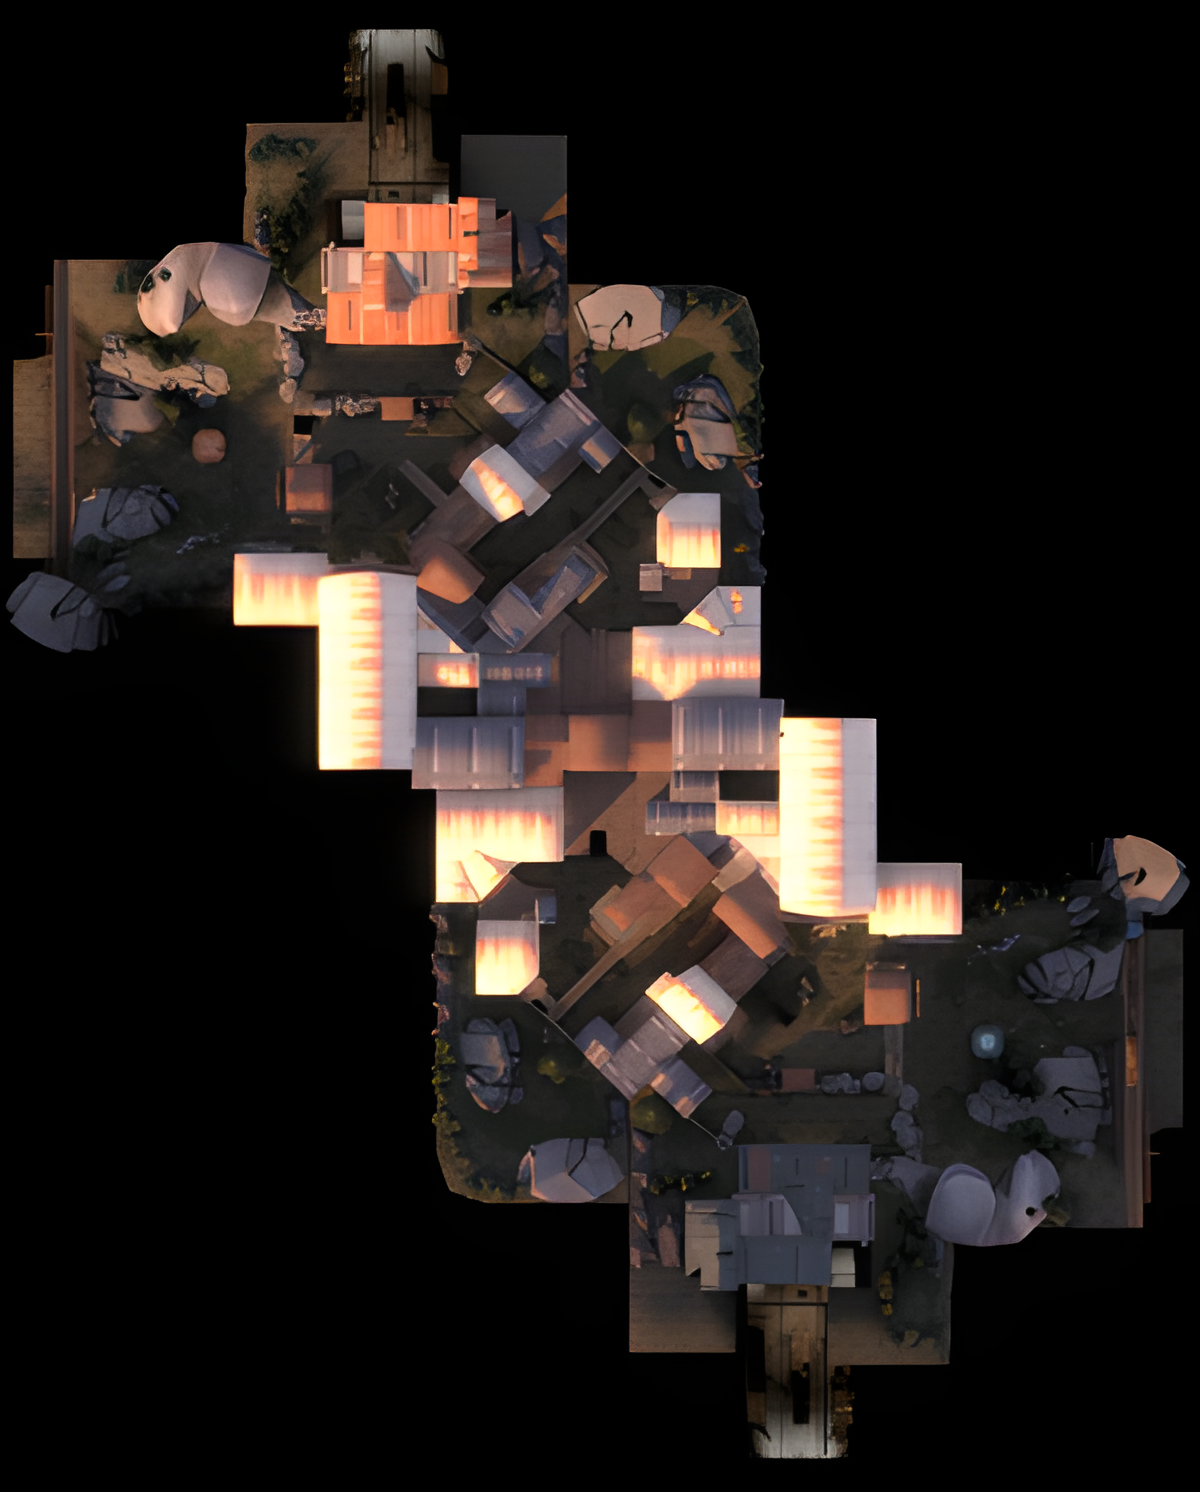
\includegraphics[height=0.4\textwidth]{Images/Thunder_Mountain_(Capture_the_Flag).png}
    }
    \quad
    \subfloat["Dust II", a Bomb Defusal map in \textit{Counter-Strike}.\label{fig:dust2}]{
        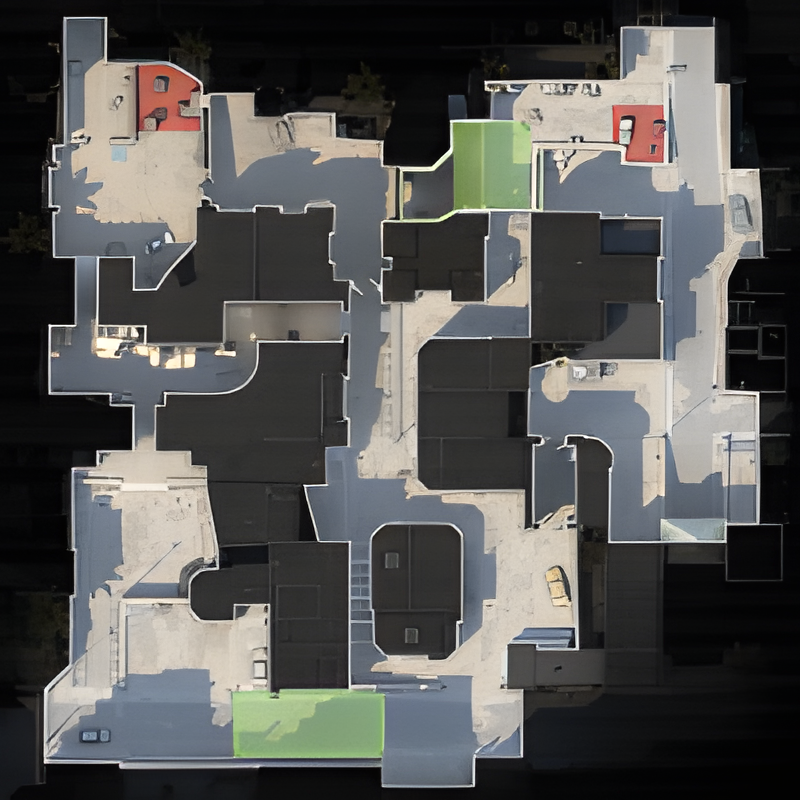
\includegraphics[height=0.4\textwidth]{Images/Dust_II.png}
    }
    \caption[Map comparison]{Comparison of a symmetrical "Capture the Flag" map with an asymmetrical "Bomb Defusal" map.}
    \label{fig:maps_compare}
\end{figure}

Even considering a single game mode, such as "deathmatch"\footnote{Game mode where players, optionally divided in teams, compete in order to score the most kills.}, the number of players in a team drastically changes the tactics that are employed, and the level design should account for that. Games that focus on 1v1 combat (e.g. \textit{Unreal Tournament 2004}) will usually have fast movement and dynamic gameplay that rewards reflexes and mechanical skills, so maps will have multiple floors with various escape routes but will be relatively small and with numerous collision points that make it hard to hide. Instead, games that are mainly played in teams (e.g. \textit{Battlefield 1942}) will have bigger maps with few collision points allowing teams to strategically position themselves to gain control of these sections.

The observations made in this section about balancing maps in competitive FPS games may seem like "common sense", however \citeauthor{johnston_common_2003}, author of the popular "Dust II" map in figure \cref{fig:dust2}, argues that the best asset a level designer has is their common sense, and uses practical examples to guide readers on how to create balanced and fun maps \cite{johnston_common_2003}.

Finally, we note that there is a lack of academic research on the topic of balancing maps in competitive FPS games, which leads to a lack of a clear methodology to follow when designing and balancing a map, having instead to rely on "common sense", trial and error, observation and experience.  

\section{Procedural content generation in games}
\label{sec:procedural_content_generation}
We refer to \textit{Procedural Content Generation} (PCG) as the process of creating game content algorithmically, rather than manually. This can be used to create levels, characters, items, quests, dialogues, and more. 

PCG has been used in games since the early days of the industry, with games like \textit{Rogue}\footnote{A.I. Design, 1980} using procedural generation to create levels, items, and enemies. The technique has helped developers create games that use less storage space and have more replayability. To this day, many successful games that span many genres employ PCG to create content, such as \textit{Minecraft}\footnote{Mojang, 2011}, \textit{No Man's Sky}\footnote{Hello Games, 2016}, the \textit{Mystery Dungeon}\footnote{Chunsoft, 1993} series or \textit{Hades}\footnote{Supergiant Games, 2020}.

\begin{figure}[hbt!]
    \centering
    \subfloat[\textit{Minecraft}\label{fig:Minecraft}]{
        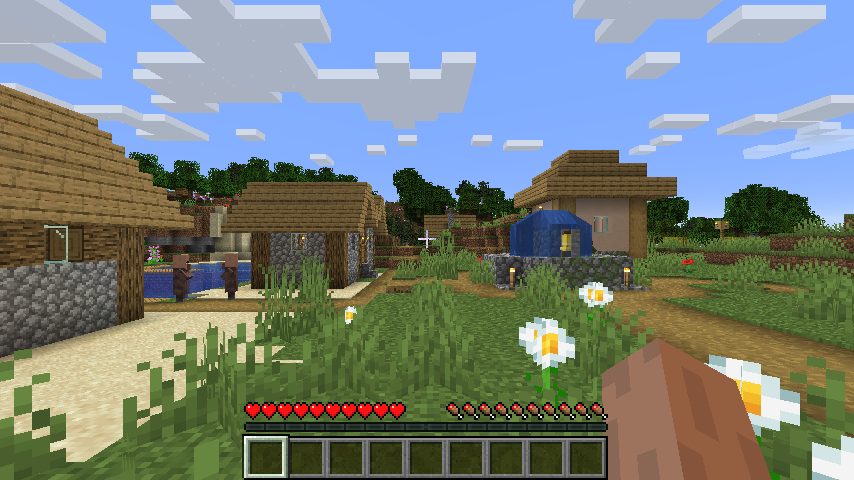
\includegraphics[height=0.2\textwidth]{Images/Minecraft.png}
    }
    %\quad
    %\subfloat[\textit{No Man's Sky}\label{fig:nms}]{
    %    \includegraphics[height=0.2\textwidth]{Images/nms.png}
    %}
    \subfloat[\textit{Pokémon Mystery Dungeon: Explorers of Sky}\label{fig:md}]{
        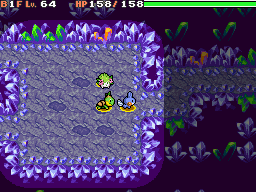
\includegraphics[height=0.2\textwidth]{Images/MD.png}
    }
    \subfloat[\textit{Hades}\label{fig:hades}]{
        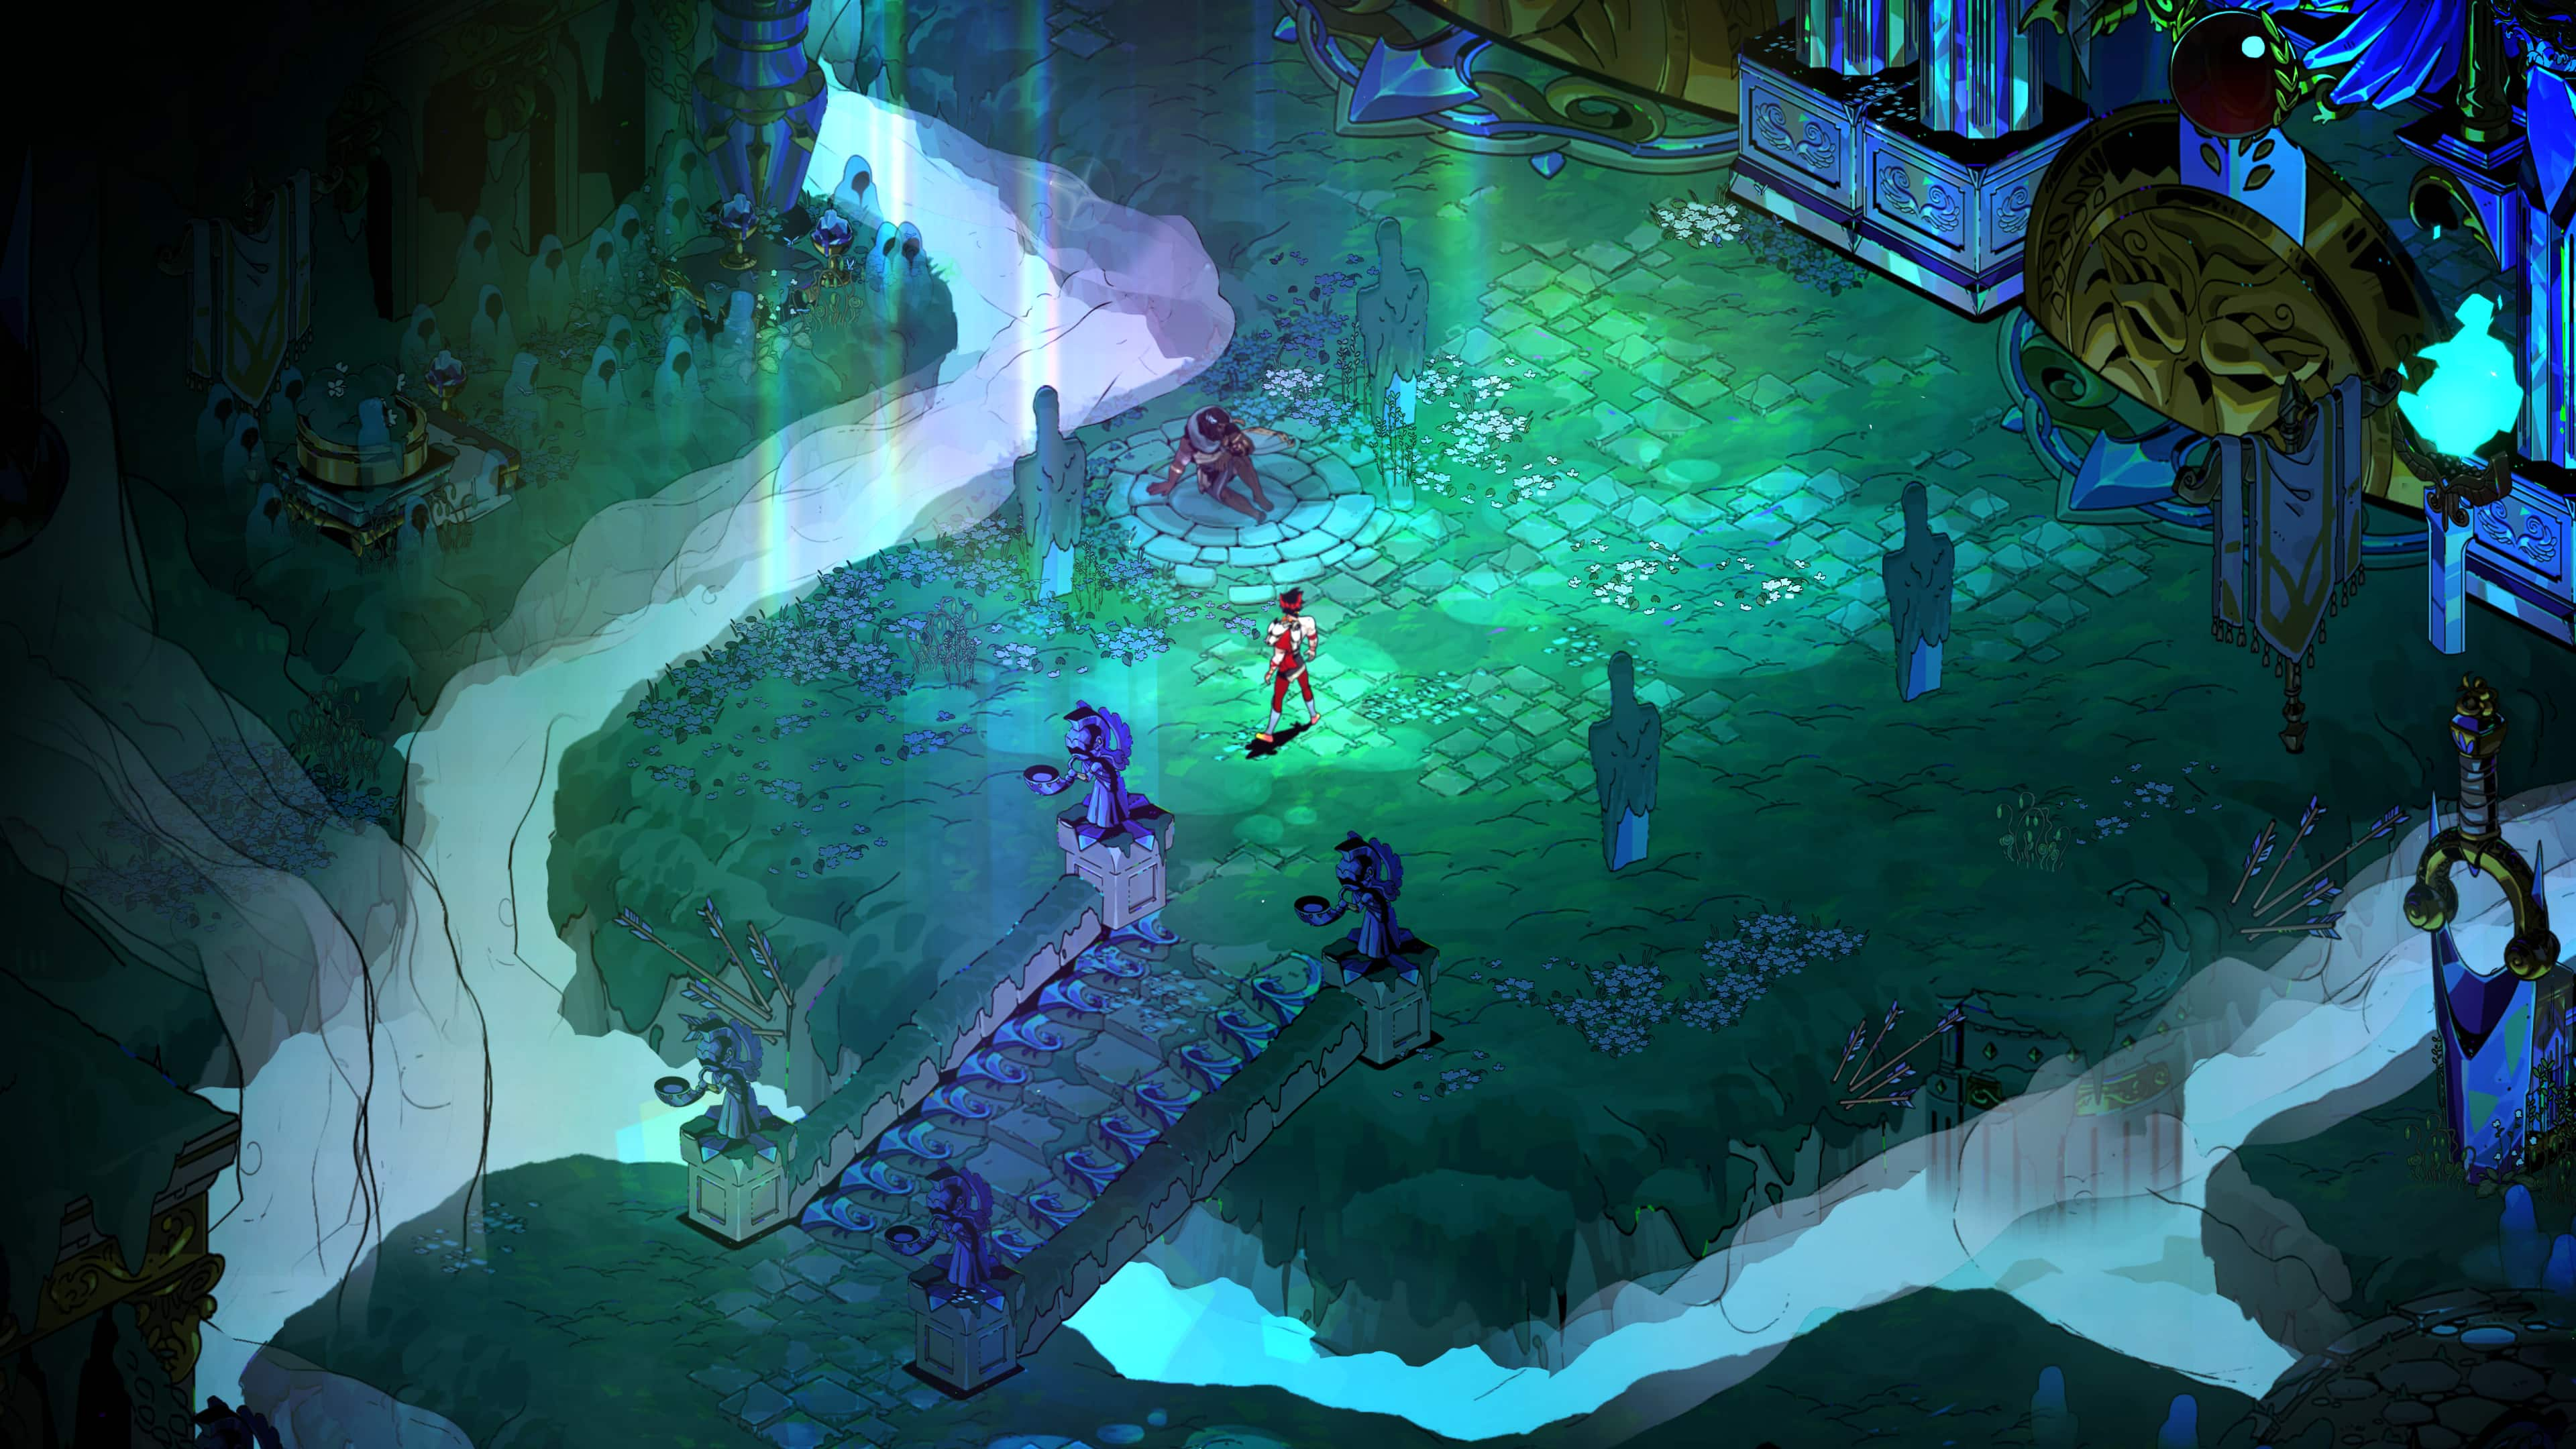
\includegraphics[height=0.2\textwidth]{Images/Hades.jpg}
    }
    \caption[PCG Games]{Examples of diverse games that use PCG to create content.}
    \label{fig:pcg_games}
\end{figure}


In the domain of FPS games PCG has mostly been used for single player games or multiplayer collaborative games. The already cited \textit{No Man's Sky} uses PCG to create an entire universe of planets, each with its own flora, fauna, and resources. \textit{Borderlands}\footnote{Gearbox Software, 2009} uses PCG to create weapons with different stats and abilities, while \textit{Deep Rock Galactic}\footnote{Ghost Ship Games, 2018} creates levels that are different each time a mission is played. However, there are no critically acclaimed multiplayer competitive games that use PCG to create levels yet.

\Citeauthor*{togelius_search-based_2010} offer a taxonomy of PCG approaches used in games by drawing some distinctions between them. First, they note the difference between \textit{online} approaches, which generate content as the game is played, and \textit{offline} approaches, which generate content during the development phase. Then they distinguish between \textit{necessary} and \textit{optional}, depending on whether the content generated is mandatory to finish the game. Another distinction is between \textit{random seeds} and \textit{parameter vectors}; the former simply takes a single seed to generate content, while the latter uses more parameters. The amount of randomness can classify an approach as either \textit{stochastic} or \textit{deterministic} and, finally, they distinguish \textit{constructive} approaches, where the content is generated once, ensuring that it is correct and good during the creation process itself, and \textit{generate-and-test}, where the content is first generated and then tested, and the algorithm is possibly repeated to produce better content. \cite{togelius_search-based_2010}

\subsection{Search based procedural content generation}
\label{subsec:search_based_pcg}
Referring to the taxonomy of PCG approaches just defined, \textit{Search Based Procedural Content Generation} (SB-PCG) is a particular case of \textit{generate-and-test} PCG, where the content is first generated, then the candidate is tested and evaluated with a \textit{fitness function}, and the generation of a new candidate depends on the result of this evaluation. \cite{togelius_search-based_2010}

\begin{figure}[hbt!]
    \centering
    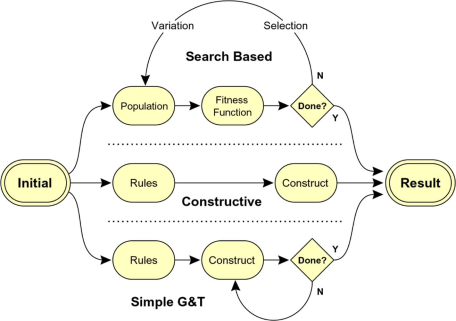
\includegraphics[width=0.6\textwidth]{Images/Togelius.png}
    \caption{Comparison of SB-PCG with constructive and generate-and-test approaches.}
    \label{fig:pcg}
\end{figure}

Among search-based PCG methods, \textit{Evolutionary Algorithms} (EA) make up most of them. \cite{togelius_search-based_2010}

An EA is a population-based optimization algorithm that mimics the process of natural selection, borrowing some concepts from biology and genetics. An algorithm of this family proceeds in cycles, often called epochs or generations. The first epoch starts with generating an initial population of candidates (or individuals), then each candidate in the population is evaluated with a fitness function and the best are selected to reproduce using crossover or mutation, creating new candidates that will replace the worst scoring individuals, giving rise to a new population, which will be the starting point of the next epoch. This process is repeated for a number of generations, and the algorithm ends when a stopping criterion is met, like a reaching certain number of generations or finding an individual with a particularly high fitness. \cite{lones_sean_2011}

An important concept that is loosely taken from biology is that of \textit{genotype} and \textit{phenotype}. EAs usually cannot work directly on the final content they are trying to generate, such as maps or 3D models, and they instead work on a low-level representation that may employ different parameters and data structures to describe the candidate's content. This representation should also allow the algorithm to apply crossover and mutation in a computationally fast and meaningful way. Each genotype is then mapped to a phenotype, which is the final content, that can be evaluated by the fitness function. \cite{togelius_search-based_2010}

Choosing the right genotype and genotype-to-phenotype mapping is crucial to the success of the algorithm, and many factors must be taken into account. 

Firstly, it is important to choose a genotype representation with the right number of parameters; an encoding having few parameters may be unable to represent the content or introduce bias in the search space, while having too many parameters may make the search space too large to be effectively explored by the algorithm\footnote{This phenomenon is called the \textit{curse of dimensionality}, referencing how having too many dimensions in a search is often detrimental to the search itself.}.
A good genotype representation will also sport good locality, meaning that a small change in the genotype should result on average in small changes in the phenotype.
A genotype encoding should also be able to represent all interesting solutions, which could be hard to achieve while avoiding the use of too many parameters. \cite{togelius_search-based_2010}

A genotype that is one to one with the phenotype (which is classified as a \textit{direct encoding}) will often lead to a search space that is too large to be effectively searched by most EAs, as we would need too many parameters to describe all the details of the phenotype. Using instead a single parameter, such as a random seed, to generate the phenotype (which is classified as \textit{indirect encoding}, as we need a complex computation to obtain the phenotype from the parameters) may lead to very poor locality, since, by definition, a good random number generator will show no correlation between the numbers generated by neighboring seed values. Choosing the correct balance between these two extremes is crucial to the success of the algorithm and requires knowledge of the domain. \cite{togelius_search-based_2010}

Another crucial factor of an EA is the fitness function. First, it must be defined what is the objective of the search, then the fitness function must be formalized. The process of defining the fitness function is complex as it requires domain-specific knowledge and depends on the objective of the search; to define how hard a level is to play we can leverage objective data, such as how many times a player dies or where he died, but formalizing abstract concepts, such as how much fun a level is to play, will surely rely on conflicting assumptions and subjective opinions, which could make our evaluation imprecise and unreliable. \cite{togelius_search-based_2010}

We can classify fitness functions in 3 categories \cite{togelius_search-based_2010}:
\begin{itemize}
    \item \textit{Direct fitness functions}, where features are extracted directly from the generated content and used to evaluate it. These functions are usually fast to compute, but many features may be hard, if not impossible, to define directly.
    \item \textit{Simulation-based fitness functions}, where an agent plays the game content generated and simulation data is recorded, which is then used to evaluate the candidate. This method is slower to compute as simulations take time to run, but it allows for a vaster range of features to be evaluated. 
    \item \textit{Interactive fitness functions}, where the candidate is evaluated by a human player and implicit (e.g. game data) or explicit (e.g. questionnaires) feedback is collected. This method avoids the inherent bias issues that arise when using bots by using human players instead, at the cost of both needing a playerbase and evolution taking longer, since the game cannot be sped up.  
\end{itemize}


\subsection{Procedural map generation in competitive FPS games}
\label{subsec:pcg_fps}
While no acclaimed commercial game uses PCG to create maps for competitive multiplayer games, some academic research has been done on the topic.

\citeauthor{cardamone_evolving_2011} have started research in this field by using search-based techniques to generate playable FPS maps for the "deathmatch" game mode of \textit{Cube 2: Sauerbraten}\footnote{Lee Salzman, Wouter van Oortmerssen, Mike Dysart, Robert Pointon, 2004}. In their work they defined four different genotypes (\textit{All-White}, \textit{All-Black}, \textit{Grid} and \textit{Random-Digger}, in figure \cref{fig:map_genomes}), and mapped each to a phenotype that can be used to generate a map for Cube 2. The candidate maps are evaluated using a simulation-based fitness function; each map is played for 10 minutes by 4 bots and the fitness is based on the \textit{average fighting time}, that is defined as the amount time passed from the moment in which the player starts to fight an opponent to the moment in which the player is killed. They argue that interesting maps will have features, such as escape routes and well-placed resources, that allow for long fights to happen. \cite{cardamone_evolving_2011}

\begin{figure}[hbt!]
    \centering
    \subfloat[\textit{All-White}\label{fig:allwhite}]{
        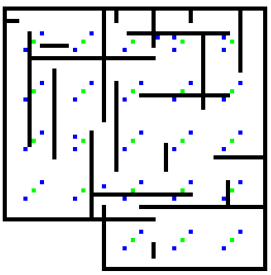
\includegraphics[height=0.2\textwidth]{Images/aw.png}
    }
    \quad
    \subfloat[\textit{All-Black}\label{fig:allblack}]{
        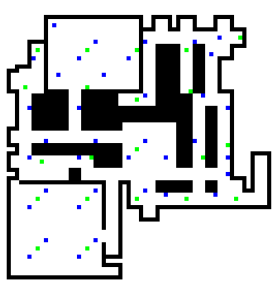
\includegraphics[height=0.2\textwidth]{Images/ab.png}
    }
    \subfloat[\textit{Grid}\label{fig:grid}]{
        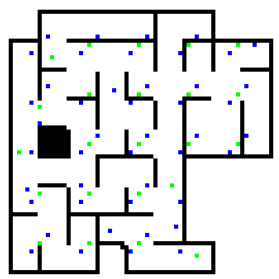
\includegraphics[height=0.2\textwidth]{Images/Grid.png}
    }
    \subfloat[\textit{Random-Digger}\label{fig:randomdigger}]{
        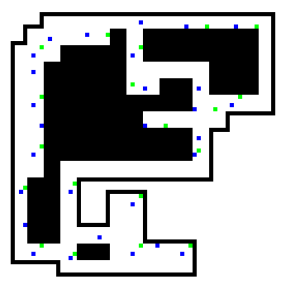
\includegraphics[height=0.2\textwidth]{Images/rd.png}
    }
    \caption[\citeauthor{cardamone_evolving_2011} example maps]{Different maps evolved by \citeauthor{cardamone_evolving_2011} with different genotypes.}
    \label{fig:map_genomes}
\end{figure}


Their work both proved the possibility of using an EA to evolve FPS maps and highlighted how different representations lead to maps with different topological characteristics, noting how some genomes were more suited to their objective.

\Citeauthor{lanzi_evolving_2014} have instead focused on evolving maps for \textit{Cube 2: Sauerbraten} that are balanced for a 1-vs-1 "deathmatch" game mode, simulated by agents which have differing skill levels and play styles. Leveraging the \textit{All-Black} genotype defined by \Citeauthor{cardamone_evolving_2011}, they employed a simulation-based fitness function based on \textit{entropy}, a measure of the match's balance based on the number of kills of each player. \cite{lanzi_evolving_2014}

\Citeauthor{olsted_interactive_2015} moved to evolving maps for the game \textit{FPSEvolver} focusing on the "Bomb Defusal" game mode, similar to that of \textit{Counter-Strike}. They argue that this game mode encourages more tactical planning and teamwork and that maps obtained by \Citeauthor{cardamone_evolving_2011} were unsuitable for this purpose, as they contained few dedicated arenas and many dead-ends. To obtain engaging maps they define a set of guidelines (named "\textit{the good engagement}") and a new genotype that by design creates layouts that adhere to these concepts, avoiding dead ends and ensuring arenas. They then employed \textit{iterative evolutionary computation} to evolve maps, requiring real users to play the maps. Users are then asked to leave binary feedback that is used to guide the evolution. \cite{olsted_interactive_2015}

\Citeauthor{loiacono_fight_2017} took an approach similar to that of \Citeauthor{cardamone_evolving_2011}, leveraging their \textit{All-Black} representation to evolve maps that foster fleeing behavior. They evolve maps that optimize a simulation-based fitness calculated using the number of times a bot loses track of an enemy who it is currently fighting. They prove that their method can generate maps that foster fleeing behavior in bots that are designed to always attack while creating maps that significantly reduce pace. \cite{loiacono_fight_2017}

\citeauthor{bari_evolutionary-based_2023} applied an EA with a multi-objective fitness approach in conjunction with the NSGA-II\footnote{NSGA-II (Non-dominated Sorting Genetic Algorithm II) is a popular multi-objective optimization algorithm that uses a fast non-dominated sorting approach and a crowding distance mechanism to ensure diversity among the solutions.} selection algorithm to optimize maps in both \textit{entropy} and \textit{pace}. \Citeauthor{bari_evolutionary-based_2023} used both the \textit{All-Black} genotype and a new grid-based genotype, \textit{Grid-Graph}, aimed at reducing the noise of the former and improving its locality. Maps were evolved for a 1-vs-1 "deathmatch" game mode in \textit{Project Arena}\footnote{\Citeauthor{ballabio_online_2018}, \citeyear{ballabio_online_2018}}, a research-oriented framework developed by \Citet{ballabio_online_2018}. While results showed successful evolution and proved that \textit{Grid-Graph} performed better in this scenario, concerns remain over the simplistic layouts generated by this representation. \cite{bari_evolutionary-based_2023}

\citeauthor{bhojan_arena_2014} instead focused on finding a faster evolution method to evolve maps in an online fashion for a "Capture the Flag" game mode in a game they developed to test their method. 
To achieve this result, they generate a map by placing tiles that either are an indoor area, an outdoor area or are inaccessible, following a rule of adjacency with pre-existing tiles. 
The map is then cleaned of artifacts and scanned with a \textit{Flood Fill}\footnote{Flood fill is an algorithm used to determine the area connected to a given node in a multidimensional array. It is commonly used in computer graphics to fill a contiguous area with a color.} algorithm to find regions, which are then connected with doors where needed. Finally, strategic points such as spawn points, flag locations and covers are placed. To allow for online evolution, the fitness function is \textit{direct} instead of \textit{simulation-based} and is aimed at evaluating features that they deem compulsory for a good map, such as connectivity, collision points and flag fairness. \cite{bhojan_arena_2014}

% [TODO: add cachia?]

\section{Quality diversity and MAP Elites}
\label{sec:qd}
The process of natural evolution has served as an inspiration for evolutionary algorithms, but it can be argued that they lag behind with respect to nature's capabilities, so much so that some argued that EAs are \textit{ad-hoc}, unprincipled or less effective than other theoretically based optimization methods. Despite these claims, as far as nature is concerned, evolution stands unmatched in power, having produced artifacts beyond the capability of any sub-field of optimization. To fill the gap between the power of evolution in nature and the performance of evolutionary methods in optimization, researchers have observed that \textit{optimization} is not the end goal of evolution, but rather that evolution is simply very good at \textit{something} that isn't \textit{optimization}, and that we may have been trying to exploit evolution in the wrong way. As a matter of fact, in nature, evolution has no unifying objective, and organisms are often rewarded for being diverse, such as when they carve a niche with less competition to increase their likelihood of survival. \cite{pugh_quality_2016}

Starting from these observations about the nature of evolution itself, a new type of search, called \textit{Quality Diversity} (QD), emerged. The goal in QD is not to find the one optimal solution, but instead to find a maximally diverse collection of individuals. When using QD approaches researchers define a \textit{behavior characterization} (BC) by selecting \textit{behavioral features} of interest, thus defining a space of possible behaviors. The underlying idea is that each part of this space is just as important as the next, while traditional optimization methods would instead focus on the most promising part of the space. When compared to other optimization methods that return multiple results, in QD methods the \textit{diversity} of individuals is measured solely based on their behavior. \cite{pugh_quality_2016}  

As a practical example we can imagine the space of possible levels in a videogame. A generic EA, whose only goal is optimization, given a suitable representation (genotype) for the actual levels (phenotype) and a way to map the two (genotype-to-phenotype mapping), would measure the fitness of each individual and discard low performing ones. A QD algorithm, instead, also defines and measures some \textit{behavioral features} of the levels, such as the level's dimension or the number of enemies, which define the space of possible behaviors. By only focusing on performance, the EA may ignore some parts of this space, such as small levels with few enemies, while the QD algorithm would aim at exploring all possibilities, which may allow it to find stepping stones for evolution.

One of the first works leaning towards QD was done by \citeauthor{lehman_exploiting_2008}, who introduced a new domain-independent algorithm to perform open-ended searches\footnote{Searches where the objective is not to find a single solution, but many diverse solutions. \cite{stanley_why_2019}} called \textit{Novelty Search} \cite{lehman_exploiting_2008}. This new approach did not place pressure to evolve towards a specific objective, but instead exclusively promoted behavioral diversity. This characteristic allows the method to perform really well in some domains, such as in deceptive problems where the fitness landscape is misleading, and the optimal solution is hard to find. While it isn't exactly a QD method, it underlines the potential of diversity-based methods. 

\Citeauthor{lehman_evolving_2011} then introduced what can be considered the first QD algorithm, \textit{Novelty Search with Local Competition (NS-LC)} \cite{lehman_evolving_2011}. This approach adds a localized fitness pressure by forcing behavioral neighbors (individuals whose features are similar, placing them close in the behavioral space) to compete, allowing for quality-based rewards to be given without asserting that a given neighborhood is better than another. This ensures that we obtain a broad population comprised of diverse behavioral niches where local competition can take place, while other non-QD approaches would instead have a notion of fitness that is global. 

\Citeauthor{mouret_illuminating_2015} introduce the term \textit{illumination algorithm} to describe algorithms whose goal is not to find the single optimal solution, but instead to find the best-performing solution at each point in the behavioral space. They also describe a new illumination algorithm called \textit{Multi-dimensional Archive of Phenotype Elites (MAP-Elites)} \cite{mouret_illuminating_2015}. 

The algorithm works by first choosing \textit{N} relevant behavioral features of our individuals, therefore defining the behavior (or feature) space. Each dimension of variation is discretized, creating an \textit{N}-dimensional grid called the \textit{archive}. The search starts by generating a number of random individuals, which are evaluated to determine both their fitness and their behavioral features. Based on the value of these features, the individuals are placed in a cell of the archive. Since the archive is formed by discretizing a finite or possibly infinite space, multiple candidates may fall in the same cell. In this case, MAP-Elites will only keep the individual with the highest fitness for each cell (the \textit{elite}), forcing local competition within niches. Then, until a stopping criterion is met (iteration count, time, etc...) MAP-Elites selects a certain number of elites from the archive, generates new individuals by applying crossover, mutation or both to each elite, evaluates their fitness and measures their features to finally place them in the archive, only keeping the best individual in each cell. When elites are mutated, the new individual may, and should, end up in a different cell of the archive, allowing distant niches to be stepping stones for each other. As a matter of fact, experiments show that the lineage of elites can often be seen traversing long paths through different regions of the map. Some cells may instead remain empty, either because no genome exists with such features or because the search failed to produce one such genome, even if one existed. \cite{mouret_illuminating_2015}

\begin{figure}[hbt!]
    \centering
    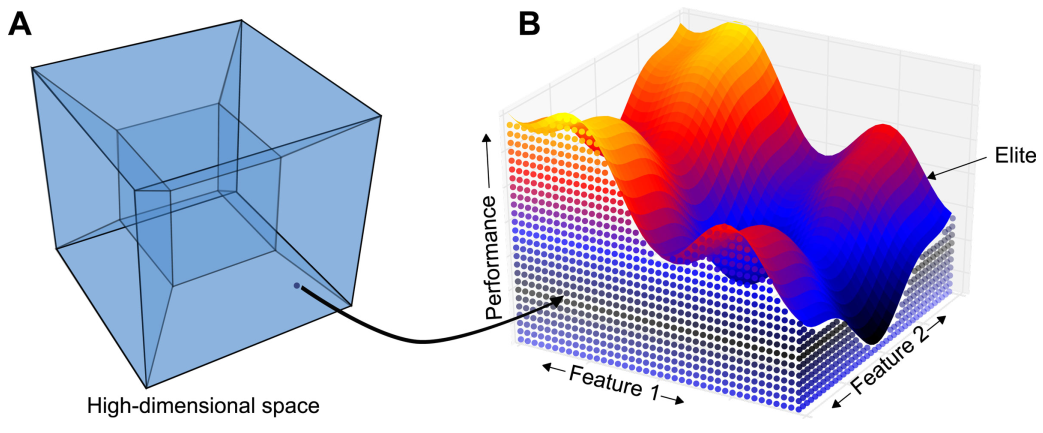
\includegraphics[width=0.7\textwidth]{Images/MAPElites.png}
    \caption{Visualization of the MAP-Elites algorithm.}
    \label{fig:mapelites}
\end{figure}

\textit{NS-LC} is also an illumination algorithm according to \citeauthor{mouret_illuminating_2015}, but they state that it is harder to understand and implement when compared to \textit{MAP-Elites}. They also show that \textit{MAP-Elites} performs empirically better than \textit{NS-LC}, by virtue of doing away with both the need to calculate the behavioral distance at each step, since it is implied in the archive itself, and with the need to maintain an archive of visited solutions separate from the current population, which NS-LS needs to avoid "cycling", the phenomenon where the population collectively moves back and forth between two regions of the behavior space. \cite{mouret_illuminating_2015}

\textit{MAP-Elites} has been used in a variety of domains and several variations have been developed in order to overcome certain limitations and adapt to specific needs. Some examples include \textit{Centroidal Voronoi Tessellations MAP-Elites} (CVT-ME) \cite{vassiliades_using_2017}, which scales the algorithm to high-dimensional spaces, \textit{Covariance Matrix Adaptation MAP-Elites} (CMA-ME) \cite{fontaine_covariance_2020} and \textit{Covariance Matrix Adaptation MAP-Annealing} \cite{fontaine_covariance_2022}, which doubles the performance of \textit{MAP-Elites} by combining the self-adaptation techniques of \textit{CMA-ES}\footnote{Covariance Matrix Adaptation Evolution Strategy is an advanced evolutionary optimization algorithm used for solving complex, non-linear, and multi-modal problems. It adapts the covariance matrix of the search distribution, allowing it to efficiently explore the search space by learning and exploiting the underlying structure of the problem.}, and \textit{Multi-Emitter MAP-Elites} \cite{cully_multi-emitter_2021}, which leverage a heterogeneous set of emitters to improve on \textit{Covariance Matrix Adaptation MAP-Elites}. Moreover, \textit{Constrained MAP-Elites} \cite{khalifa_talakat_2018}, \textit{MAP-Elites with Sliding Boundaries} (MESB) \cite{fontaine_mapping_2019} and other alternatives have been developed in the context of procedural content generation in games, which we will examine in the next section.

\subsection{Quality Diversity for procedural content generation in games}
\label{subsec:qd_pcg}
Among the many applications of QD methods across disciplines, such as optimization, robotics and machine learning, particularly relevant is their application to procedural content generation in games.

Quality Diversity is an appealing approach to PCG in games for a variety of reasons. 
While QD can generate a diverse set of high performing solution, constructive algorithms and machine learning methods produce instead a single artifact, search-based PCG is only concerned with the best-performing solution, and other declarative approaches, such as generative programming, while fast, lack the ability to control the diversity of the generated content. Moreover, QD considers more than one dimension of interest and leverages local competition instead of global competition, making it capable of exploring the fitness landscape better than other search-based methods. This allows QD to avoid deceptive fitness landscapes that may arise from the inherently difficult task of designing a fitness function. QD also generates, as a byproduct, the large set of artifacts needed to perform \textit{Expressivity Analysis}\footnote{The analysis of the output in terms of styles and variety of artifacts generated by the chosen approach, which can highlight biases of the generator towards specific types of content. \cite{gravina_procedural_2019}}, making it possible to run this process online during generation. Finally, QD is especially well-suited for mixed-initiative content design and offers \textit{explainability}\footnote{Explainable AI for Designers is an important research area that aims to aid the game designer in understanding AI algorithms applied to games. \cite{gravina_procedural_2019}} to the game designer thanks to its capability of showing a solution's lineage. \cite{gravina_procedural_2019} 


Notably, \textit{MAP-Elites} has been used to generate content for a variety of genres and some variations of the technique have been developed to fit specific needs. 

\citeauthor{khalifa_talakat_2018} have used \textit{MAP-Elites} to generate levels for bullet hell games. To that end, they developed a description language, \textit{Talakat}, capable of describing bullet hell levels, and a new technique called \textit{Constrained MAP-Elites}, which fuses the \textit{MAP-Elites} algorithm with the \textit{Feasible-Infeasible 2-Population} (FI2Pop) genetic algorithm\footnote{Genetic algorithm where two populations are kept, one of feasible and one of infeasible individuals. The feasible population is evolved to better its fitness, while the infeasible one to reduce their constraint violations, allowing the method to find more stepping stones. \cite{kimbrough_feasibleinfeasible_2008}} \cite{kimbrough_feasibleinfeasible_2008}. This new algorithm is able to evolve bullet hell levels described with \textit{Talakat} by keeping in each cell of the archive a population of feasible and infeasible levels, which are those levels that either satisfy a number of constraints or don't, and by evolving both populations simultaneously. Keeping two populations allows \textit{Constrained MAP-Elites} to find stepping stones between levels that would have otherwise been discarded immediately. Instead of defining a complex fitness function that describes "good" levels, a number of metrics are chosen as different dimensions of the \textit{Constrained MAP-Elites} and only playability is considered for the fitness function. \cite{khalifa_talakat_2018}

Several works have instead focused on platforming games. \Citeauthor{khalifa_intentional_2019} use \textit{Constrained MAP-Elites} to evolve a variety of playable \textit{Super Mario Bros.} levels which revolve around a specific game mechanic, using and comparing different simulation approaches to generate them \cite{khalifa_intentional_2019}. \Citeauthor{warriar_playmapper_2019} implemented \textit{PlayMapper}, a variation on the MAP-Elites algorithm, that is able to generate \textit{Super Mario Bros.} levels of different sizes and grants a significant amount of control over their generation, in contrast with popular black-box" AI techniques \cite{warriar_playmapper_2019}. \citeauthor{fontaine_illuminating_2021} apply some \textit{MAP-Elites} methods to illuminate the latent space of a \textit{Generative Adversarial Network (GAN)}\footnote{The latent space of a GAN is the space from which points are taken as input to generate new artifacts, and usually it's a vector. During training, the GAN learns how to map each point to generate an artifact.} trained on scenes from \textit{Super Mario Bros}. They focus on assessing the performance of QD algorithms on the task of generating scenes for \textit{Super Mario Bros.} with some specific characteristics \cite{fontaine_illuminating_2021}.

Another genre that has been the focus of QD research is that of "Zelda-like"\footnote{Games like The \textit{Legend of Zelda} (Nintendo EAD, 1986), where a player character traverses a world, fights enemies and beats dungeons made up of rooms with locked doors and keys.} adventure games, set in dungeons. 
\citeauthor{alvarez_empowering_2019} have used a new QD algorithm called \textit{Interactive Constrained MAP-Elites} to evolve dungeon rooms in \textit{Evolutionary Dungeon Designer} (EDD), a "mixed-initiative co-creativity"\footnote{The process of creating something by repeatedly having a human and a machine inspire each other through reciprocal stimuli.} tool. They leverage EDD's fitness and FI2Pop algorithm to develop an interactive version of \textit{Constrained MAP-Elites}, where the user guides the search towards satisfying results by choosing the features to explore and providing feedback on generated rooms \cite{alvarez_empowering_2019}. 
\citeauthor{charity_mech-elites_2020} searched for levels with specific mechanics in the \textit{GVG-AI Framework}'s games \cite{perez-liebana_general_2019}, which include a "Zelda-like" game \cite{charity_mech-elites_2020}. 
\Citeauthor{gonzalez-duque_finding_2020} used the \textit{Intelligent Trial-and-Error}\footnote{A form of Bayesian Optimization that uses MAP-Elites to generate the priors for a Gaussian Process} algorithm to perform \textit{Dynamic Difficulty Adjustment}, successfully producing levels of the desired difficulty for a "Zelda-like" game \cite{gonzalez-duque_finding_2020}. \citeauthor{viana_illuminating_2022} focused on generating entire levels, instead of single rooms, along with locked doors missions and enemy placement using MAP-Elites, while maintaining dungeon quality and providing a set of diverse levels \cite{viana_illuminating_2022}.

Some research has been done in the realm of puzzle games. \Citeauthor{charity_baba_2020} developed \textit{Baba is Y'all}, a mixed-initiative version of \textit{Baba is You}\footnote{Hempuli, 2019} where players design levels in collaboration with the machine. The game allows players to edit \textit{Baba is You} levels, similar to \textit{Super Mario Maker}\footnote{Nintendo EPD, 2015}, with the added goal of filling the archive of the underlying MAP-Elites algorithm, where levels are placed based on the combination of mechanics (rules) that are activated when solving them. The system can propose various starting levels for the user to edit based on what is already in the archive and what's currently missing to help players fill the archive \cite{charity_baba_2020}. 

MAP-Elites has also been used to generate powerful but diverse decks for \textit{Hearthstone}\footnote{Blizzard Entertainment, 2014}. \citeauthor{fontaine_mapping_2019} noted that \textit{MAP-Elites} uniformly divides the behavior space, however this can lead to a mismatch with the true distribution of the behavior space, which would result in a less effective illumination. Moreover, they argue that knowing \textit{a priori} this distribution can be hard or even impossible. To solve these issues, they propose \textit{MAP-Elites with Sliding Boundaries} (MESB), a variation of MAP-Elites where boundaries between cells are not placed uniformly based on the value of the features, but instead are dynamically placed at certain percentage marks of the distribution. A remap frequency is specified, meaning that the boundaries are periodically recalculated, allowing for a good estimation of the distribution of the search space. \cite{fontaine_mapping_2019}

Quality Diversity methods have yet to be applied to FPS games, be them singleplayer or multiplayer, which is where our research places itself.

\section{Summary}
\label{sec:ch1_summary}
In this chapter we have outlined the main concepts of level design in games, with a specific focus on competitive FPS games and academic research on them. We then explored the definition of "game balance", focusing on competitive games, and discussed the importance of map design in competitive FPS games to achieve balance. Furthermore, we have also discussed the main concepts of Procedural Content Generation in games, focusing on search-based methods and Evolutionary Algorithms in particular, and how they have been used to generate maps for FPS games. We have then introduced the concept of Quality Diversity and the MAP-Elites algorithm, explaining how they came to be and how they differ from traditional optimization methods. Finally, we have reviewed the main works that have used Quality Diversity methods to generate content for different genres of games, highlighting some relevant MAP-Elites variants such as MAP-Elites with Sliding Boundaries.



\chapter{Frameworks and tools}
\label{ch:tools}
In the following chapter we are going to present the two frameworks that we leveraged to perform our research and the tools they offer.

First we will take a look at \textit{Project Arena}, a light and modular research-oriented framework developed by \citeauthor{ballabio_online_2018} in \textit{Unity}. The framework is used to generate maps and to simulate matches, and it has been later extended to support bots by \citeauthor{bari_evolutionary-based_2023}. We will present its main component and features to give an insight on how we have used it to evaluate and evolve maps.

Then we will present Pyribs, a Python library that aids researchers in using state-of-the-art Quality Diversity algorithms and in implementing new algorithms using pyribs's modular conceptual Quality Diversity framework called \textit{RIBS}. We will delve into the \textit{RIBS} framework to understand how its main components work and how they have been used.

\section{Project Arena}
\label{ch:project_arena}


\subsection{Description and motivations}
\label{sec:pa_description}
Academic research on the topic of procedural map generation in FPS games has mostly used \textit{Cube 2: Sauerbraten} \cite{cardamone_evolving_2011}\cite{lanzi_evolving_2014}\cite{loiacono_fight_2017}; while undoubtedly a powerful option thanks to its rich map editor, its ability to run in headless mode and its open-source nature, modifying the source code of a game is never an easy task. Moreover, the game was never developed with the explicit intent of being used in academic research, which makes it cumbersome to run tasks such as user studies, with parties involved needing to download the game on their machines, which would often discourage participants.

\textit{Project Arena} \cite{ballabio_online_2018} is a research-oriented framework developed by \citeauthor{ballabio_online_2018} in \textit{Unity}\footnote{A popular game engine developed by Unity Technologies.} with the main goals of being light and modular. Using a game engine lends the framework to being modified more easily, since it is widely known in the industry, and also allows the game to be easily built for WebGL, allowing the game to be run in a browser. 

One issue with the framework, compared to \textit{Cube 2: Sauerbraten}, was the lack of bots, which are essential to perform simulations in search-based PCG methods. To solve this issue, \citeauthor{bari_evolutionary-based_2023} developed bots that can be used in the framework \cite{bari_evolutionary-based_2023}. This way games can be simulated, and data can be recorded to be later analyzed or to be used for fitness calculations.

\subsection{Framework overview}
\label{sec:pa_overview}

\subsubsection{Map Representation}
\label{subsec:map_representation}

Maps can be seen as matrices of orthogonal \textit{tiles} and are internally represented as matrices of characters. A tile in the map corresponds to a cell in the matrix, and depending on the character in the cell the tile can be a wall, a floor or an object on the floor. Maps can also have multiple levels, in which case they are represented as lists of matrices, with each representing a level.

Two different formats can then be supplied to the framework, which are converted to the internal format just described. The first is a textual representation, where each line corresponds to a row of the matrix, and a blank line is used to divide multi-level maps. The second is a modified version of the \textit{All-Black} genotype originally defined by \citeauthor{cardamone_evolving_2011}, where rooms are encoded as triplets with the center's coordinates and size, corridors as triplets with the starting position's coordinates and length and objects as triplets with the object's coordinates and type. Multi-level maps are represented by dividing levels with special characters.

\subsubsection{Structure}
\label{subsec:structure}
The framework is organized in a series of modular "Managers" that handle different aspects of the game, aided by various other modules.

The \textbf{Game Manager} is the main manager and is responsible for the behavior of a game, with different Game Managers being used for different game modes, which include \textit{Duel}, a classic deathmatch, \textit{Target Rush}, where waves of enemies must be eliminated, and \textit{Target Hunt}, where a series of enemies must be eliminated within a time limit. The Game Manager is responsible for managing the lifecycle of a game, including setup, map generation, countdown, play and end.

The \textbf{Map Manager} generates or loads a map, assembles it and displaces objects on the map, relying on other entities to perform these tasks. The Map Manager is further differentiated into the Single-Level Map Manager, which handles single-level maps, the Multi-Level Map Manager, which handles multi-level maps, and the All-Black Map Manager, which handles maps in the multi-level \textit{All-Black} format.

The \textbf{Map Generator} is used to generate maps, with different versions being used to generate different topologies. The \textit{Cellular Generator} employs a parametric cellular automaton to generate a map, the \textit{Divisive Generator} uses instead a binary space partitioning algorithm, the \textit{Digger Generator} uses a random digger algorithm and the \textit{All-Black Generator} parses maps in the \textit{All-Black} format. The \textbf{Stairs Generator} then places or validates stairs for multi-level maps.

The \textbf{Map Assembler} aids the assembly of the map and can either assemble meshes or prefabs.

The \textbf{Object Displacer} is used to place objects, such as spawn ammunition, on the map based on the characters in the matrix. It also populates a dictionary that is used to decide where to place spawn points, which are stored by the \textbf{Spawn Point Manager}.

The \textbf{Experiment Manager} is a stand-alone module that helps researchers run user-based studies. Experiments are first defined with an optional \textit{tutorial}, with a collection of \textit{studies}, each divided in multiple \textit{cases} containing each a pool of maps, which are to be validated, played on a specific game mode and finally with an optional survey. Once defined, the \textit{Experiment Manager} selects studies and cases in a round-robin fashion to assign players and runs the experiment, either online or offline. During the experiment, information is logged (e.g. the map's information, the game's information) and can be later downloaded from the server.

Besides managers, other relevant components include \textbf{Entities}, which refer to any \textit{agent} that takes part in a match, and include the player, opponents and targets, \textbf{Weapons} (Assault Rifle, Shotgun, Sniper Rifle, Rocket Launcher and Laser Gun) which are highly parameterized, \textbf{Objects} such as decorations and spawners of health packs and ammunition. 

\subsubsection{Bots}
\label{subsec:bots}

\citeauthor{bari_evolutionary-based_2023} developed bots for the framework with the aim of creating a modular system that would facilitate maintenance and modifications to the bots. \cite{bari_evolutionary-based_2023}

The architecture of the bots is structured in layers, with the first being the \textbf{Sensing Layer}. This layer receives raw data from the game world so that other layers can process it to determine the bot's behavior. It is responsible for sightings of players, objects and obstacles, hearing sounds and sensing damage received.

The \textbf{Knowledge Base Layer} analyzes the data and provides tactical information, which is then used to make decisions. The layer is divided in modules responsible for keeping a knowledge base of enemy locations, objects' locations and last visited map locations. This information is then used by the \textit{Navigation System} to calculate the path to a given destination. This layer is also responsible for introducing a delay between the bot's sight of an enemy and its actual detection, to simulate human reaction times.

The \textbf{Decision Making Layer} is responsible for choosing the objective to pursue and the action plan to follow in order to achieve it, based on the bot's state and knowledge. To allow the bot to be easily understood and modified, the action plans that the bots are graphically defined by behavior trees and are followed to achieve the goal defined by the current state. The possible states are \textit{Wander}, \textit{Fight}, \textit{Collect pickup} and \textit{Search enemy}. 

Finally, the \textbf{Actuator Layer} is responsible for actuating the physical actions of the bot, such as moving and rotating the camera, as a response to the decisions taken.

An important feature of the bots is their parameterization; this allows bots to be used to simulate players with different skill set, play-styles and skill level. In particular, we can modify a general \textit{skill score}, that expresses how skilled a bot is on a scale from 0 to 1, and many \textit{ability scores}, which define how skilled a bot is on a scale from 0 to 1 in a specific characteristic, such as reflexes, aiming skill and speed. These characteristics have been used to define three bot profiles which are the \textit{Shotgun}, an aggressive and agile player focused on close-quarters combat, the \textit{Sniper}, a patient player focused on long-range combat with exceptional aiming skills, and the \textit{Assault}, a balanced player who excels in medium-range combat.

\subsubsection{Data gathering}
\label{subsec:pa_data_gathering}
To perform experiments of any kind, data must be able to be gathered from matches. To that end, the framework can collect a variety of data which is saved to be later analyzed and enriched outside the framework.

The framework collects the following raw data related to the match:

\begin{itemize}
    \item \textit{Time to engage}: The interval from the end of one combat event to the start of the next, or, at the beginning of the match, the time from respawn to the first combat encounter.
    \item \textit{Time in fight}: The total time a bot spends actively engaged in combat, including the period spent searching for an enemy after losing visual contact.
    \item \textit{Number of sights}: The total number of combat engagements.
    \item \textit{Time between sights}: The time elapsed between losing sight of an enemy and detecting it again, measured for each combat event.
    \item \textit{Number of re-sights}: The number of times an enemy is re-detected after initially becoming undetected.
    \item \textit{Time to surrender}: The time taken for a bot to stop searching for an enemy after losing track of it.
    \item \textit{Number of retreats}: The number of instances where a bot ceases searching for an enemy after losing sight of it.
\end{itemize}

The framework also records the following data for each entity:

\begin{itemize}
    \item \textit{Frags}: Number of kills performed. 
    \item \textit{Deaths}: Number of deaths. 
    \item \textit{Shots}: Number of bullets fired. 
    \item \textit{Hits}: Number of times a projectile shot hit an entity (including itself).
\end{itemize}

Besides raw data, the framework also calculates some metrics that are useful to analyze the design of maps. These include:

\begin{itemize}
    \item \textit{Entropy}: As defined and used by \citet{lanzi_evolving_2014} and \citet{loiacono_fight_2017}, entropy is a measure used to infer the map's balance, calculated as follows:
    \begin{equation}
        entropy = \sum_{i=1}^{n} - \left(\dfrac{k_i}{k_{tot}}\right) \log_2 \left(\dfrac{k_i}{k_{tot}}\right)
    \end{equation}
    Where for each bot $i$ the number of kills $k_i$ is divided by the total number of kills $k_{tot}$ and multiplied by the logarithm of the result. The entropy is then the sum of these values and is meant to represent how balanced a match on a certain map has been, given that, as we already discussed in \cref{sec:balance}, the map's design could greatly influence the match's result. Possible values range from 0 to 1, with 1 representing a balanced match and 0 meaning a wildly unbalanced match.
    \item \textit{Pace}: The frequency of combat engagements normalized between 0 and 1, calculated as follows:
    \begin{equation}
        pace = 2 * \dfrac{1}{1 + \exp \left(-5 * \dfrac{NumberOfFights}{\sum TimeToEngage}\right)} - 1
    \end{equation}
    This sigmoid function computes values close to 0.9 when the average time to engage is 3 seconds.

\end{itemize}

\section{Pyribs}
\label{ch:pyribs}
\subsection{Description and motivations}
\label{sec:pyribs_description}
The \textit{pyribs} library\footnote{\url{https://pyribs.org/}} is a Python library that aids researchers in using state of the art Quality Diversity algorithms and in implementing new algorithms using pyribs's modular conceptual Quality Diversity framework called \textit{RIBS}.

\textit{pyribs} aims at solving two challenges found within the Quality Diversity community: a lack of a conceptual framework applicable to  recently developed QD algorithms that also incorporate evolution strategies, gradient ascent and Bayesian optimization, and a lack of an implementation of said framework in a software that supports many users. \textit{pyribs} attempts to do so by introducing the \textit{RIBS framework}, explained in \cref{sec:ribs}, and by providing a Python implementation of it. \cite{tjanaka_pyribs_2023}

Other libraries exist in the field of Quality Diversity, written in different languages and serving different purposes. \textit{Sferes\textsubscript{v2}} \cite{mouret_sferesv2_2010} is a C++ framework designed for high performance focusing on Evolutionary Algorithms as a whole, including Quality Diversity algorithms. The use of templates makes the library efficient at the cost of accessibility. 
\textit{QDpy} \cite{cazenille_qdpy_2018} is a Python library focused solely on QD algorithms which offers building blocks that can be composed into different algorithms, but requires the user to supply an evaluation function, limiting its flexibility. 
\textit{pymap\_elites} \cite{mouret_python3_2019}  is a reference implementation of the MAP-Elites algorithm and of some variants, such as CVT-ME \cite{vassiliades_using_2017}, in Python, but it is not designed to be a general-purpose QD library.
Finally, \textit{QDax} \cite{lim_accelerated_2022} focuses on implementing QD algorithms, EAs, and Reinforcement Learning algorithms for hardware accelerators\footnote{Hardware accelerators are specialized hardware designed to perform specific tasks more efficiently than general-purpose hardware. Some examples of hardware accelerators include GPUs and TPUs}.

We chose \textit{pyribs} for our research because of its dedicated focus on Quality Diversity algorithms, its comprehensive selection of state-of-the-art methods, its user-friendly interface, its visualization methods and its flexibility for extension and customization. 

\subsection{RIBS framework}
\label{sec:ribs}

To solve the challenge of a lack of a conceptual framework, \citeauthor{tjanaka_pyribs_2023} introduce the \textit{RIBS} framework, whose goal is to be capable of implementing any QD algorithm, from MAP-Elites to Novelty-Search, and all variations that may use evolutionary strategies, such as  \textit{Covariance Matrix Adaptation MAP-Elites} \cite{fontaine_covariance_2020}, gradient ascent, or Bayesian Optimization.

The framework is made up of three main components: the \textit{Archive}, the \textit{Emitters} and the \textit{Scheduler}.

The \textbf{Archive} is the component responsible for storing solutions. It allows for the addition of new solutions and querying of existing ones. When solutions are added, the archive provides feedback on the insertion, such as whether the new solution improved an existing elite or its novelty score\footnote{The novelty score is typically defined as the average distance in the measure space from the solution to its k-nearest neighbors in the archive}, depending on its type.

The \textbf{Emitters} are responsible for generating new solutions. They can be asked for new solutions and may require to be told the fitness they achieved in order to update their internal algorithm. 
For example, the basic \textit{MAP-Elites} \cite{mouret_illuminating_2015} algorithm uses one emitter which simply chooses a random elite in the archive and either mutates it or applies crossover to it and doesn't require to be told anything since it has no internal state to maintain. 
\textit{CMA-ME} \cite{fontaine_covariance_2020}, instead, uses the \textit{CMA-ES} algorithm to generate new solutions, which requires to be told the fitness of the solution it generated in order to update its internal state.

The \textbf{Scheduler} has two roles: facilitate the interactions between the archive and the emitters and choose which emitter to use between the pool, based on their previous performance.
A Scheduler implements an "ask-tell" interface; when the "ask" method is called, the scheduler chooses some emitters and asks them for new solutions, which are returned to the user. Later, the user is expected to call the "tell" method of the scheduler, providing the fitness of the solutions, which the scheduler uses to update the emitters' internal state by telling them.

It is worth noting that the framework does not include facilities to evaluate the solutions; this step is left to the user to allow for maximum flexibility. This is useful in the case of Search-Based Procedural Content Generation, where the evaluation of a solution may require running a simulation, as in the case of generating maps for a game. The user can thus ask for new solutions, perform the genotype-to-phenotype mapping, run the simulation using the phenotype, evaluate the solution and tell the results. 

This modular design allows for the implementation of a variety of QD algorithms, many of which are already supported by the library, but also allows for more solutions to be explored. Creating novel QD algorithms is also facilitated by the framework, since the user can rely on existing components and modify only some to create a new algorithm.

\section{Summary}
\label{sec:tools_summary}
In this chapter we have presented the two frameworks that we have used to perform our research. We have presented an overview of \textit{Project Arena}, a research-oriented framework developed by \citeauthor{ballabio_online_2018} in \textit{Unity}, focusing on why it was chosen, its main advantages compared to other popular games used for research, such as \textit{Cube 2}, its internal structure and the metrics that can be gathered from matches. We have also presented the bots developed by \citeauthor{bari_evolutionary-based_2023} and their architecture, focusing on the parameterization that allows for different play-styles and skill levels. We have then presented \textit{pyribs}, a Python library that aids researchers in using state-of-the-art Quality Diversity algorithms and in implementing new algorithms using pyribs's modular conceptual Quality Diversity framework called \textit{RIBS}, focusing on the motivations behind its development and the \textit{RIBS} framework, its main components and how they interact. We have also discussed the flexibility of the framework and how it allows for the implementation of new QD algorithms. 

\chapter{FPS map's representations and features}

In the following chapter we will discuss the genome representation that we have decided to use in order to later evolve maps using a Quality Diversity algorithm. We will discuss two existing genomes, \textit{All-Black} and \textit{Grid-Graph}, and two new genomes that we have introduced, \textit{Point-Line} and \textit{SMT-Genome}. 

Following, we will describe all the features that we have extracted from the maps, divided into \textit{emergent} and \textit{topological}, and how we have calculated them. 

\section{Map representation}
\label{sec:map_genomes}
As discussed in \cref{subsec:search_based_pcg}, in order to evolve maps, we have to define a suitable representation (genome) which can be mapped to the actual map (phenotype) to be evaluated by the framework, which is \textit{Project Arena} in our case. In the following section we will discuss the genomes we examined and how they map to a common phenotype that can be used by the framework to generate the actual maps to be evaluated through simulations.
\subsection{All-Black genome}
\label{subsec:all_black}
The \textit{All-Black} genome was first introduced by \citet{cardamone_evolving_2011} and later used in more academic research \cite{lanzi_evolving_2014} \cite{loiacono_fight_2017} \cite{bari_evolutionary-based_2023}. \citeauthor{cardamone_evolving_2011} proposed four different genomes, \textit{All-Black}, \textit{All-White}, \textit{Grid} and \textit{Random-Digger}, and while on average All-White performed best, future research has instead focused on All-Black, given its capability of producing maps which more closely resemble topologies of man-made maps by using explicitly the concepts of rooms/arenas and corridors.

In the \textit{All-Black} genome, the map contains only wall tiles initially, and walkable spaces are "carved" in the form of \textbf{rooms} and \textbf{corridors}.

The All-Black genome can be defined as a list of:
\begin{itemize}
    \item $NR$ triplets <$x$, $y$, $s$> where each represents a \textbf{room}, with $x$ and $y$ being the coordinates of the lower left corner of the room and $s$ being the size of the room.
    \item $NC$ triplets <$x$, $y$, $l$> where each represents a \textbf{corridor}, with $x$ and $y$ being the coordinates of the lower left corner of the corridor and $l$ being the length of the corridor. The length can be positive or negative, encoding, respectively, horizontal or vertical corridors.
\end{itemize}
The genome is thus encoded by a list of $NR$ + $NC$ triplets, where the first $NR$ encode rooms, and the remaining $NC$ encode corridors.

When a genome is created, rooms and corridors are placed at random on the map. This could lead to unconnected regions, which are eliminated when converting the genome to the phenotype as follows: the room closest to the center is chosen and any room or corridor which intersects it is added to the phenotype. This process is repeated until no more rooms or corridors intersect with any of the rooms or corridors in the phenotype, ensuring that only rooms that are connected to the center are kept.

The genome supports mutation by randomly replacing \textit{rooms} and \textit{corridors} and crossover by randomly exchanging \textit{rooms} and \textit{corridors} between two genomes.

As already noted by \citeauthor{bari_evolutionary-based_2023}, \textit{All-Black} has two main problems. The first is a \textit{lack of locality}: the change of a single number of the genome, such as a corridor length's, can lead to a large change in the phenotype's topology. This lack of locality impedes the performance of Evolutionary Algorithms, as discussed in \cref{subsec:search_based_pcg}. The second is \textit{redundancy}: different genomes may result in the same final map; as an example, we could have a genome with a room fully contained in another bigger room, thus several genomes would result in the same final map if the smaller room is moved while still being fully contained in the bigger room. Another problem is that resulting maps are on average very noisy, often having many dead ends and confusing topological features.

\begin{figure}[hbt!]
    \centering
    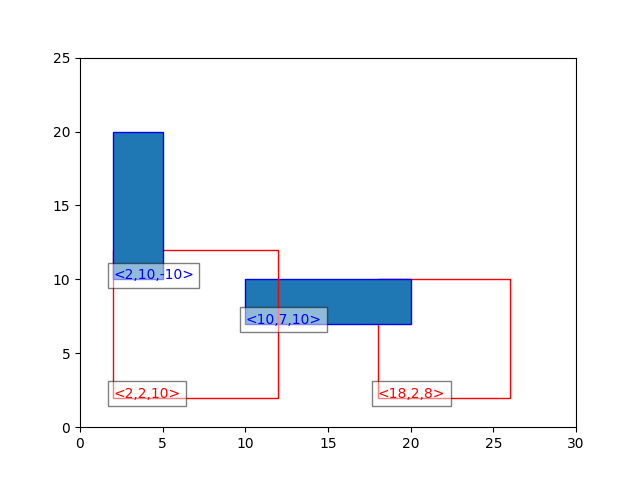
\includegraphics[width=0.65\textwidth]{images/ABGenome.png}
    \caption[All-Black example]{An example of a simple All-Black genome}
    \label{fig:all_black}
\end{figure}

\subsection{Grid-Graph genome}
\label{subsec:grid_graph}
\textit{Gird-Graph} was introduced by \citeauthor{bari_evolutionary-based_2023} with the aim of overcoming All-Black's problems.

The genome is similar to \textit{All-Black} in the sense that the map is initially full of walls and \textit{rooms} and \textit{corridors} are then placed on it. Given a map made of $H$ x $W$ tiles, Grid-Graph divides the map into an $R$ x $C$ grid where each cell occupies $r$ x $c$ tiles. 

Each cell can either contain one or no \textbf{room}, which is an axis aligned rectangle, defined by the width of the room $w$ (between 1 and $c$), the height of the room $h$ (between 1 and $r$) and the coordinates of the lower left corner of the room relative to the cell, so an $x$ (between 0 and $c$ - $w$ - 1) and a $y$ (between 0 and $r$ - $h$ - 1). Thus, the genome will contain an $R$ x $C$ matrix of rooms, where a room in cell ($i$, $j$) is defined with the above quartet of values, or a special value \textit{Nil} if no room is present in the cell.

Rooms can be connected by \textbf{corridors} if they are placed in horizontally or vertically adjacent cells. This is encoded in the genome via a single boolean value for each pair of horizontally or vertically adjacent cells, meaning that we have an $R$ x ($C$ - 1) matrix of boolean values for horizontal corridors, where the value in cell ($i$, $j$) indicates whether rooms in cell ($i$, $j$) and ($i$, $j$ + 1) are connected by a horizontal corridor, and a ($R$ - 1) x $C$ matrix of boolean values for vertical corridors, where the value in cell ($i$, $j$) indicates whether rooms in cell ($i$, $j$) and ($i$ + 1, $j$) are connected by a vertical corridor.

Similarly to \textit{All-Black}, the genome is converted to the phenotype by placing rooms and corridors on the map and keeping only the connected portion closest to the center of the map, eliminating all other unconnected regions. The genome supports mutation by randomly changing \textit{rooms} and \textit{corridors} and crossover by randomly exchanging \textit{rooms} and \textit{corridors} between two genomes.

\begin{figure}[hbt!]
    \centering
    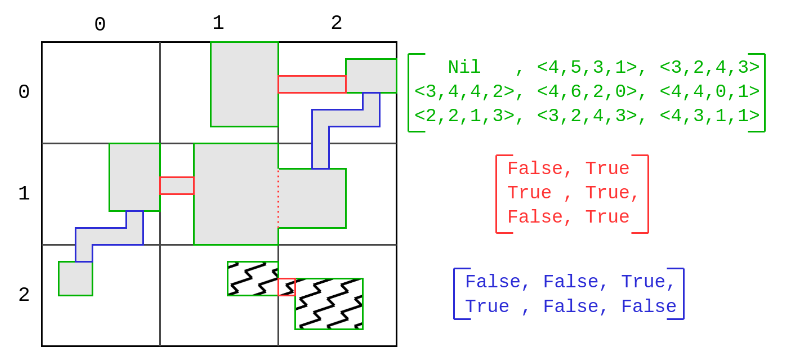
\includegraphics[width=0.85\textwidth]{images/GridGraph.png}
    \caption[Grid-Graph example]{An example of a simple Grid-Graph genome where rooms are shown in green, vertical corridors are shown in blue and horizontal corridors in red. Disconnected parts are filled with a zig-zagged line. Taken from \cite{bari_evolutionary-based_2023}.}
    \label{fig:grid_graph}
\end{figure}

\citeauthor{bari_evolutionary-based_2023} argues that \textit{Grid-Graph} overcomes the problems of \textit{All-Black}. The genome is more compact and less redundant, as rooms have no way to overlap. However, locality is still a problem (although in a more controlled way, since connected regions are separated only if their respective corridor is removed) and the resulting maps appear very simple, with the possible number of layouts being seemingly very limited.

\subsection{Point-Line genome}
\label{subsec:point_line}

We introduce in this work the \textit{Point-Line} genome, which takes its inspiration from \citet{olsted_interactive_2015}. The key idea that we borrow is that of defining explicitly the topology of the map by defining couples of points that are connected by L-shaped corridors.

Similarly to All-Black, the map is initially full of walls, and \textit{rooms} and \textit{corridors} are placed in it. 

The genome is defined as a list of $P$ \textbf{point couples}, where each point is defined by its $x$ and $y$ coordinates. Two points will be connected by an L-shaped corridor in the phenotype, and an additional value $c$ defines the orientation of the L-shaped corridor connecting the two: 0 indicates that, from the point that is leftmost and lower of the two, the corridor first extends horizontally and then vertically, while 1 indicates the opposite. Each point also serves as the coordinates for the center of an associated \textbf{room}, which is an axis aligned square of size $s$. The room is thus a square with each side being long $2s$. When the size is 0, no room is associated to the point.

The genome can be seen as a list of $P$ septets <$x_1$, $y_1$, $x_2$, $y_2$, $s_1$, $s_2$, $c$>, where the first four values are the coordinates of the two points, the next two are the size of the rooms associated to the points and the last is the orientation of the corridor connecting the two points. 

When the genome is converted to the phenotype, rooms are placed on the map and the corridors are drawn to connect the points. 

As already noted for the other representations, the resulting map may not be fully connected, which is similarly solved by keeping only the connected portion of the map that is closest to the center. The genome supports mutation by randomly changing the \textit{point couples}, the \textit{rooms} associated to the points or the orientation of the corridors, and crossover by randomly exchanging \textit{point couples} between two genomes.

We believe this genome to be capable of representing a wider range of topologies when compared to \textit{Grid-Graph}, while still being easily readable to the human player. Locality is improved with respect to \textit{All-Black} since rooms are explicitly connected by corridors, meaning that to remove a connection there needs to be a significant difference between the genomes, and simply moving a room also moves the corridor, keeping them connected. By coupling points and reusing coordinates between corridors and rooms, the genome is also more compact than \textit{All-Black}. We also believe that defining corridors by their start and end gives both long and short corridors an equal chance to appear, allowing \textit{Point-Line} to be more likely to explore different design, while long corridors in \textit{All-Black} are rarely found due to the need of placing a series of corridors to form a longer one.  However, the genome does not solve the problem of redundancy, as rooms can still overlap. This solution thus places itself in a sort of middle ground between \textit{All-Black} and \textit{Grid-Graph}, with the aim of combining the best of both.

\begin{figure}[hbt!]
    \centering
    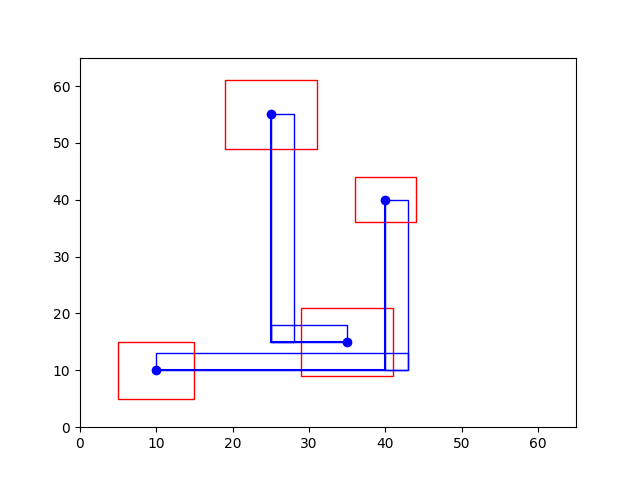
\includegraphics[width=0.65\textwidth]{images/PointGenome.png}
    \caption[Point-Line example]{An example of a simple Point-Line genome where points, L-shaped connections and related corridors raw shown in blue and rooms are shown in red.}
    \label{fig:point_line}
\end{figure}

\subsection{SMT-Genome}
\label{subsec:smt_genome}

We also introduce in this work the \textit{SMT-Genome}, which is inspired by \citet{whitehead_spatial_2020}. In their work, they propose to use a satisfiability modulo theories (SMT) solver\footnote{Satisfiability modulo theories is the field concerned with the satisfiability of mathematical formulas involving real numbers and complex data structures. An SMT solver is a tool that tries to determine said satisfiability.} to place rooms of varying dimension in a 2D map. 

Similarly to all other genomes we have discussed, the map is initially full of walls, and \textit{rooms} and \textit{corridors} are placed in it.
The genome is defined by a list of $R$ axis-aligned rectangular \textbf{rooms}, where each room is defined only by its width and height, and a list of $L$ \textbf{lines}, which are defined by two points in the 2D maps that are logically connected by a line, forming a segment. Finally, the genome also includes a parameter for minimum separation, $s$, which determines the minimum distance between rooms' borders. 

The genome is thus a list of $R$ + $L$ + 1 elements, where the first $R$ elements are couples of values representing rooms, the following $L$ are quadruplets with the coordinates of the two points of the line and the last is the minimum separation.

Differently from the other genomes, rooms are not encoded with their position, as their position is determined by the SMT solver. Thus, when the genome needs to be converted to a phenotype, a position has to be found for each room. This is done following an approach similar to that of \citet{whitehead_spatial_2020}; a number of linear constraints\footnote{Expressions where all the terms are of the first order, thus no exponents, logarithms, etc. appear.} are defined where the terms are the $x$ and $y$ coordinates of each room's upper left corner. We then used Pythons \textit{Z3}\footnote{\url{https://pypi.org/project/z3-solver/}} library to solve the system of constraints, which returns the coordinates of the upper left corner of each room.

The first class of constraints ensures that all rooms are placed inside the map's border. 
\begin{equation}
    \begin{split}
            \forall r_i \in Rooms,\: x_{r_i} >= 0 \land x_{r_i} <= width_{map} - width_{r_i} \\ \land y_{r_i} >= 0 \land y_{r_i} <= height_{map} - height_{r_i}
    \end{split}
\end{equation}

The second ensures that no two rooms overlap.

\begin{equation}
\label{eq:room_overlap}
    \begin{split}
        \forall r_i, r_j \in Rooms\, \mid\,  r_i != r_j, \\
        y_{r_j} <= y_{r_i} - height_{r_j} - s\: \lor \\
        y_{r_i} <= y_{r_j} - height_{r_i} - s\: \lor \\
        x_{r_j} <= x_{r_i} - width_{r_j} - s\: \lor \\
        x_{r_i} <= x_{r_j} - width_{r_i} - s
    \end{split}
\end{equation}

The equation \cref{eq:room_overlap} ensures that no two rooms overlap by asserting, in order, that the room $j$ must be located either fully above, below, to the left or to the right of room $i$, at a distance of at least $s$.

The last class of constraints ensures that rooms are placed close to the lines defined by the genome. To achieve this, lines are associated to a static common parameter called $linewidth$ and their $slope$ is calculated. We must note that Z3 requires integer coefficients, so many interesting slopes between 0 and 1 would be truncated; to solve this, the vertical $y$ dimension is scaled up by a factor of 1000, and then de-scaled at the end. The constraints are defined as follows:

\begin{equation}
\label{eq:room_line}
    \begin{split}
        &\forall l_i \in Lines,\, \forall r_j \in Rooms, \\
        &y_{r_j} \leq slope_{l_i} * (x_{r_j} - x_{end_{l_i}} + linewidth) + y_{end_{l_i}} \:\land \\
        &y_{r_j} \geq slope_{l_i} * (x_{r_j} - x_{end_{l_i}} - linewidth + width_{r_j}) + y_{end_{l_i}}
    \end{split}
\end{equation}

\textit{Z3} will solve all these constraints and return the coordinates of the upper left corner of each room, if one such solution exists.

Once the rooms' positions are defined, rooms must be connected using corridors. Similarly to \citeauthor{whitehead_spatial_2020}, first we define connections between two rooms by drawing a Delaunay triangulation\footnote{A type of triangulation (which is the subdivision of a planar object into triangles) which ensures that, for a set of points, that no circumcircle (circle passing through a triangle's vertices) contains any other point.} with the rooms' positions, obtaining a graph where an edge represents that the two rooms are connected by a corridor. Subsequently, we only keep a subset of connections by drawing a minimum spanning tree (MST)\footnote{A tree that connects all the vertices of a graph with the minimum possible total edge length.} on the triangulation, ensuring that we keep a connected graph. Rooms that are connected by an edge in the MST are then connected physically by a corridor in the phenotype. Corridors are built following a deterministic procedure, based on the rooms' relative positions, to avoid introducing another layer of randomness. 

We noted that the maps generated via this method were not sufficiently connected; \citeauthor{whitehead_spatial_2020} was interested in dungeon designs, where an SMT could suitably represent a linear layout with a start, an end and some optional rooms and paths, but multiplayer FPS maps require more complex topologies that entail loops, arenas and alternate routes, as discussed in \cref{sec:level_design}. We thus decided to add connections between rooms via a heuristic; given a line, rooms that are intersected by it are connected by a corridor, if they weren't already connected.

\begin{figure}[hbt!]
    \centering
    \subfloat[Example of a simple SMT-Genome without added corridors]{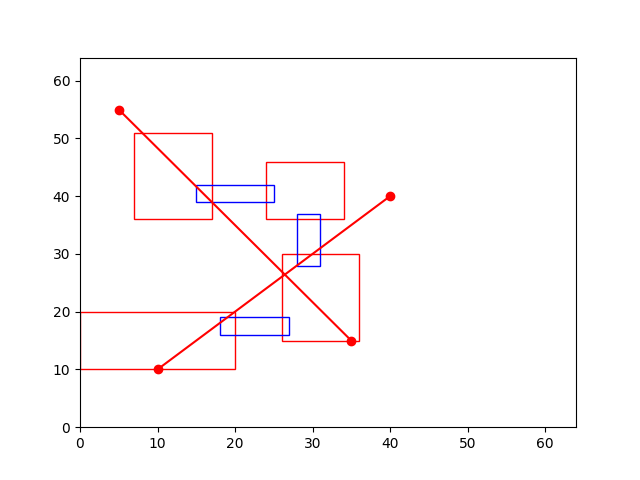
\includegraphics[width=0.45\textwidth]{images/SMT_NotAdded.png}}
    \qquad
    \subfloat[Example of a simple SMT-Genome with added corridors]{\includegraphics[width=0.45\textwidth]{images/SMT_added.png}}
    \caption[SMT-Genome lines]{An example of how corridors are added between rooms intersected by a line.}
    \label{fig:smt_genome}
\end{figure}

The genome supports mutation by randomly changing the rooms and lines and crossover by randomly exchanging rooms and lines between two genomes.

It must be noted that, differently from the other genomes, the SMT-Genome is not deterministic; while we can set a seed in \textit{Z3}, the result of the solving process may still vary when run on the same genome due to the nature of the solver itself. This could be a problem as it could lead to poor locality. Genomes may also have no feasible solution, in which case we are forced to discard it.

\begin{figure}[hbt!]
    \centering
    \subfloat{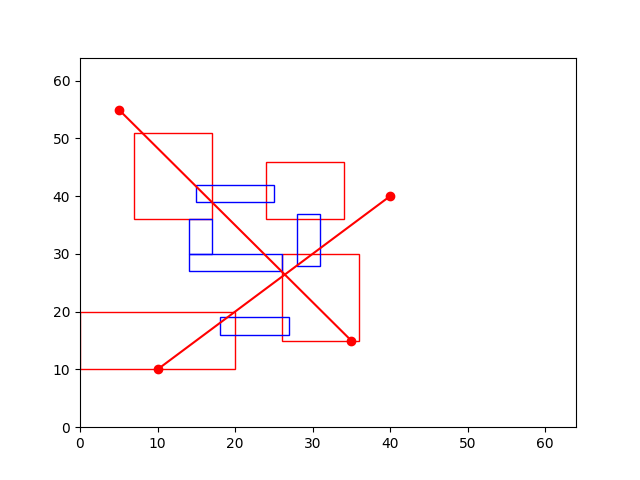
\includegraphics[width=0.45\textwidth]{images/SMT_Added.png}}
    \qquad
    \subfloat{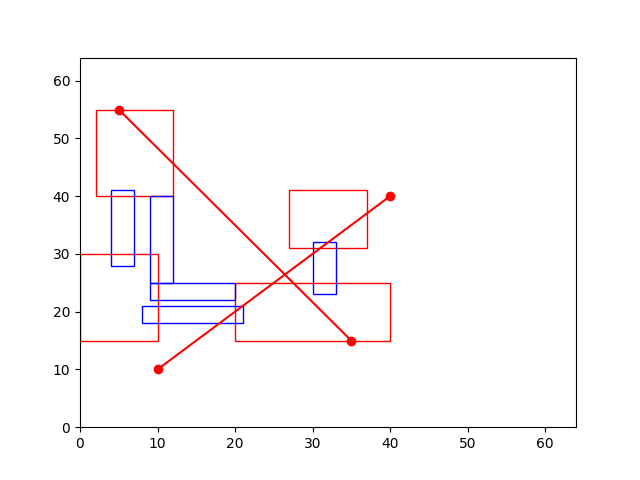
\includegraphics[width=0.45\textwidth]{images/SMT_Added_2.png}}
    \caption[SMT-Genome determinism]{Examples of how the same SMT genome may lead to different results.}
    \label{fig:smt_genome_determinism}
\end{figure}

\subsection{Common Areas-Phenotype}
All genomes are transformed to a common phenotype, called \textbf{Areas-Phenotype}. This phenotype is then supplied to \textit{Project Arena} where it is transformed into the internal textual representation used to build the actual map. This phenotype describes the map as rectangles of walkable tiles placed on a grid where each tile is a wall.

The \textit{Areas-Phenotype} is an object which contains:

\begin{itemize}
    \item \textit{MapWidth}: The map's width
    \item \textit{MapHeight}: The map's height
    \item \textit{MapScale}: The scale of the map, used by the framework to enlarge or shrink the map's size.
    \item \textit{Areas}: A list of areas, where each area is a rectangle full of walkable spaces defined by:
    \begin{itemize}
        \item \textit{BottomRow}: The $y$ coordinate of the bottom row of the area
        \item \textit{TopRow}: The $y$ coordinate of the top row of the area
        \item \textit{LeftCol}: The $x$ coordinate of the left column of the area
        \item \textit{RightCol}: The $x$ coordinate of the right column of the area
        \item \textit{IsCorridor}: A boolean value indicating whether the area is a corridor or a room
    \end{itemize}
\end{itemize}

\clearpage
\section{Features}
\label{sec:features}
To accomplish our goal, we tried to define a variety of different features that could describe a map from. We identified two main categories of features:  \textit{emergent} and \textit{topological}.

\subsection{Emergent features}
\label{subsec:emergent_features}
We define \textbf{emergent} features as those that "emerge" from actual gameplay and that are not directly tied to the map's topological features, such as the number of kills. The map's layout will surely influence the result of the match, but we cannot predict emergent features solely from the map's topology, and instead we must rely on simulations to gather them.

These features utilize the metrics defined in \cref{subsec:pa_data_gathering} and are defined as follows:
\begin{itemize}
    \item \textit{entropy}: A measure used to infer the map's balance, calculated as follows:
    \begin{equation}
        entropy = \sum_{i=1}^{n} - \left(\dfrac{k_i}{k_{tot}}\right) \log_2 \left(\dfrac{k_i}{k_{tot}}\right)
    \end{equation}
    Where for each bot $i$ the number of kills $k_i$ is divided by the total number of kills $k_{tot}$ and multiplied by the logarithm of the result, and the entropy is then the sum of these values. Possible values range from 0 to 1, with 1 representing a balanced match and 0 meaning a wildly unbalanced match.
    \item \textit{ratio}: The ratio of the number of kills to the number of deaths.
    \item \textit{pace}: The frequency of combat engagements normalized between 0 and 1, calculated as follows:
    \begin{equation}
        pace = 2 * \dfrac{1}{1 + \exp \left(-5 * \dfrac{NumberOfFights}{\sum TimeToEngage}\right)} - 1
    \end{equation}
    This sigmoid function computes values close to 0.9 when the average time to engage is 3 seconds.
    \item \textit{fightTime}: The average time the bots spend exclusively fighting, calculated as follows for $N$ bots:
    \begin{equation}
        fightTime = \dfrac{  \sum_{i}^{N} \left(timeInFight_i - timeBetweenSights_i - timeToSurrender_i\right) }{ N * gameLength}
    \end{equation}
    \item \textit{pursueTime}: The average time the bots spend pursuing an enemy, which include the time spent looking for it, calculated as follows for $N$ bots:
    \begin{equation}
        pursueTime = \dfrac{  \sum_{i}^{N} \left(timeInFight_i\right) }{ N * gameLength}
    \end{equation}
    \item \textit{sightLossRate}: The average time between losing sight of an enemy and detecting it again, calculated as follows for $N$ bots:
    \begin{equation}
        sightLossRate = \dfrac{  \sum_{i}^{N} timeBetweenSights_i }{ \sum_{i}^{N} timeInFight_i}
    \end{equation}
    \item \textit{targetLossRate}: The number of retreats compared to the number of fights, calculated as follows for $N$ bots:
    \begin{equation}
        targetLossRate = \dfrac{  \sum_{i}^{N} numberOfRetreats_i }{ \sum_{i}^{N} numberOfFights_i}
    \end{equation}
    \item \textit{killDiff}: The difference between the number of kills and the number of deaths.
\end{itemize}

Besides these, we also define some features leveraging the data gathered by the framework, particularly the raw data about kill's positions, death's positions and bots' positions (sampled at a fixed interval of 0.5s) during the match. For each bot, we plot each position on a discretized grid representing the map, obtaining a heatmap of the positions of the kills and deaths. We then apply a Gaussian filter to the heatmap to smooth it, and calculate the following features on each of the three heatmaps:

\begin{itemize}
    \item \textit{maxValue}: The maximum value of the heatmap.
    \item \textit{averageLocalMaximaValue}: The average of the values of all local maxima of the heatmap.
    \item \textit{stdLocalMaximaValue}: The standard deviation of the values of all local maxima.
    \item \textit{quantile25}: The first quartile of the heatmap's values.
    \item \textit{quantile50}: The second quartile (median) of the heatmap's values.
    \item \textit{quantile75}: The third quartile of the heatmap's values.
    \item \textit{localMaximaNumber}: The number of local maxima of the heatmap.
    \item \textit{localMaximaTopDistance}: The distance between the two local maxima with the highest values.
    \item \textit{localMaximaAverageDistance}: The average distance between all local maxima.
    \item \textit{coverage}: The percentage of the walkable map covered by the heatmap, meaning that the value is not 0 in that position.
\end{itemize}

\begin{figure}[hbt!]
\label{fig:heatmaps_example}
    \centering
    \subfloat{{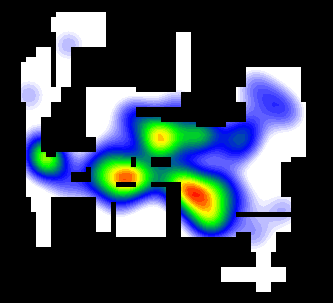
\includegraphics[width=0.4\textwidth]{images/Deaths_Heat_Example.png} }}
    \qquad
    \subfloat{{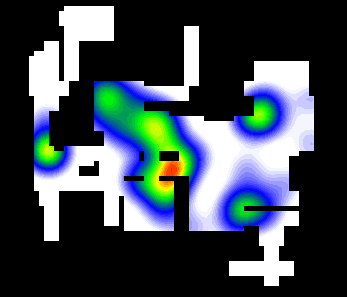
\includegraphics[width=0.4\textwidth]{images/Kill_Heat_Example.png} }}
    \caption[Heatmaps example]{An example of a heatmap of the deaths' positions (left) and the kills' positions (right)}
\end{figure}

We also utilize the kills and deaths' positions to calculate the "kill traces". A kill trace is the path of the bullet that killed a bot, and we can obtain them by connecting the position of the killer to the position of the killed bot. We then calculate the following features on the kill traces:

\begin{itemize}
    \item \textit{maxTraces}: The longest kill trace.
    \item \textit{averageTraces}: The average length of the kill traces.
    \item \textit{quantile25Traces}: The first quartile of the kill traces' lengths.
    \item \textit{quantile50Traces}: The second quartile (median) of the kill traces' lengths.
    \item \textit{quantile75Traces}: The third quartile of the kill traces' lengths.
\end{itemize}

\begin{figure}[hbt!]
\label{fig:kill_traces_example}
    \centering
    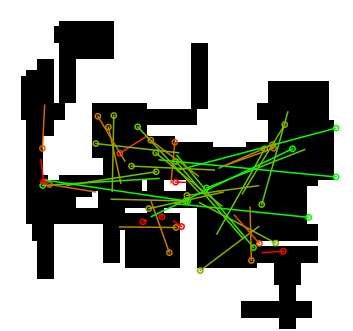
\includegraphics[width=0.4\textwidth]{images/Traces_Example.png}
    \caption[Kill traces example]{An example of the kill traces over a match, with the killer bot's position marked with a circle and brighter colors indicating longer traces.}
\end{figure}

\subsection{Topological features}
\label{subsec:topological_features}
Topological features are those that describe the map's topology, and they can be directly inferred from the map itself without the need of simulations. The simplest example is the following feature: 

\begin{itemize}
    \item \textit{area}: The number of tiles that are walkable compared to the total number of tiles in the map.
\end{itemize}

In order to extract interesting topological features it was clear that the map's representations as matrices of tiles would not be directly suitable, so we decided to convert the map to a graph representation with the aim of identifying rooms as nodes and add edges between rooms that are directly connected by a corridor. To achieve this goal, we looked at two methods for room segmentation. 

The first is the "Distance Transform-based Segmentation" approach used in \citep{bormann_room_2016}. First, we compute the Euclidean distance transform\footnote{\raggedright\url{https://docs.scipy.org/doc/scipy-0.14.0/reference/generated/scipy.ndimage.morphology.distance_transform_edt.html}} on the map, which is represented as a grid of tiles that are either walkable or walls, obtaining a map of distances. Then we locate the local maxima that are at least 3 tiles apart. These points serve as the room center coordinates that are used as markers for a Watershed\footnote{\raggedright\url{https://scikit-image.org/docs/stable/api/skimage.segmentation.html\#skimage.segmentation.watershed}} algorithm, using the negative distance map as basin. The identified rooms are then used as nodes to build the graph, where edges are added between rooms with common borders. Figure \cref{fig:dt_segmentation} shows an example of the result.

\begin{figure}[H]
    \centering
    \subfloat[The rooms identified by the algorithm]{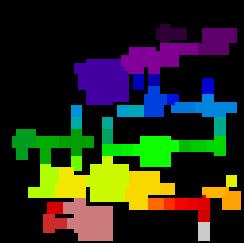
\includegraphics[height=0.4\textwidth]{images/graph_dist_color.png}}
    \qquad
    \subfloat[The graph obtained connecting adjacent rooms]{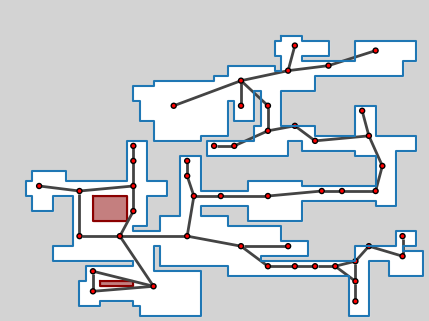
\includegraphics[height=0.4\textwidth]{images/graph_dist.png}}
    \caption[Distance Transform Segmentation example]{An example of the Distance Transform-based Segmentation}
    \label{fig:dt_segmentation}
\end{figure}

The second is the approach for region decomposition based on line segment Voronoi diagrams detailed by \citet{perkins_terrain_2010}, which we will describe here briefly. Starting from a map represented by a grid of walkable or wall tiles, we use a flood fill algorithm to identify the external wall (which we ensure is always a single polygon by adding a wall border to the map) and all obstacles (contiguous areas of walls inside a walkable part of the map) and transform them into polygons. Then we create a Voronoi diagram\footnote{\raggedright\url{https://pypi.org/project/pyvoronoi/}} of the line segments of the polygons, removing from the diagram secondary edges and edges inside the obstacles' polygons. The Voronoi diagram is transformed then into a graph, and for each node we compute a \textit{radius}, defined as the minimum distance from the node to the nearest obstacle. We use this radius to prune the graph by iteratively removing leaves whose radius is smaller than their parent's. Then we identify \textit{regions} (\textit{rooms}, in our case) and \textit{chokepoints} based on the degree of a node and its radius and, to simplify the graph, we merge adjacent rooms using some heuristics. The process and its results are shown in figure \cref{fig:voronoi_region_decomposition}.

\begin{figure}[hbt!]
    \centering
    \subfloat[The map as a grid.]{
\includegraphics[height=0.3\textwidth]{images/graph_v_1.png}}
    \qquad
    \subfloat[The map represented by polygons.]{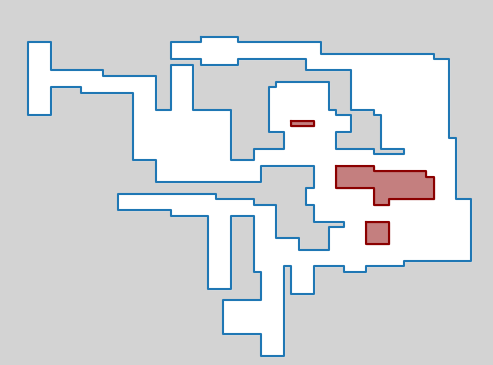
\includegraphics[height=0.3\textwidth]{images/graph_v_2.png}}
    \qquad
    \subfloat[The line segment Voronoi diagram.]{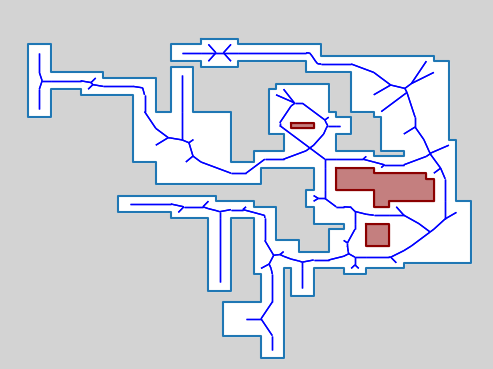
\includegraphics[height=0.3\textwidth]{images/graph_v_3.png}}
    \qquad
    \subfloat[The graph obtained by the diagram after pruning.]{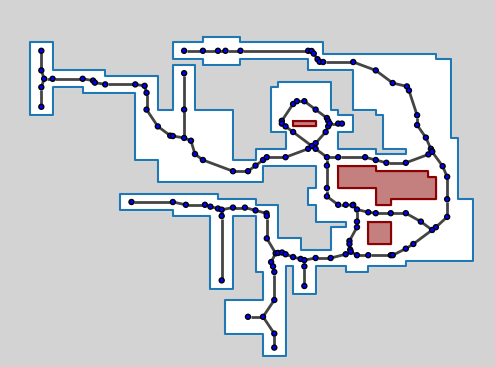
\includegraphics[height=0.3\textwidth]{images/graph_v_4.png}}
    \qquad
    \subfloat[Rooms (red) and chokepoints (yellow) identification.]{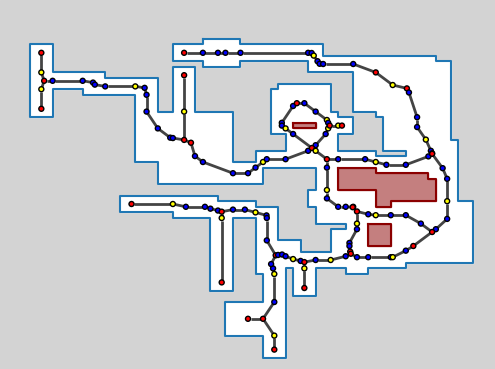
\includegraphics[height=0.3\textwidth]{images/graph_v_5.png}}
    \qquad
    \subfloat[The final graph after rooms are heuristically merged.]{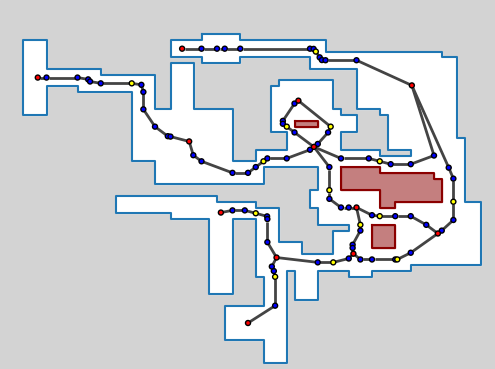
\includegraphics[height=0.3\textwidth]{images/graph_v_6.png}}
    
    \caption[Voronoi Region Decomposition example]{An example of the Voronoi Region Decomposition process.}
    \label{fig:voronoi_region_decomposition}
\end{figure}

While results are similar, the Voronoi-based approach felt more suited to our needs, providing a graph that structurally resembles the map's topology and distinguishes relevantly between rooms and corridors. Moreover, the Distance Transform-based approach is often unable to identify multiple connections between two rooms, which is a common and important feature of FPS maps. In figure \cref{fig:graph_comparison} we show a comparison to facilitate the understanding of the problem at hand.

\begin{figure}[hbt!]
    \centering
    \subfloat[Distance Transform-based Segmentation]{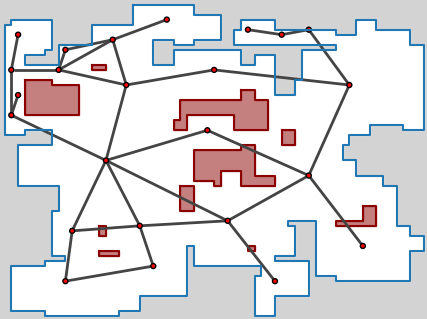
\includegraphics[width=0.45\textwidth]{images/graph_compare_dist.png}}
    \qquad
    \subfloat[Voronoi Region Decomposition]{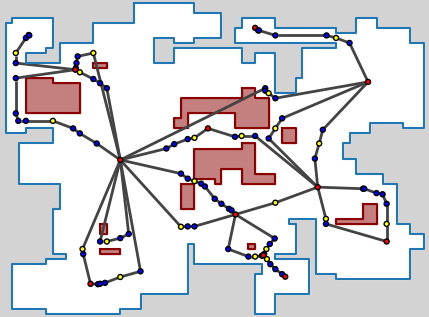
\includegraphics[width=0.45\textwidth]{images/graph_compare_vor.png}}
    \caption[Graph comparison]{A comparison between the graphs obtained with the two methods. Notice how in the bottom-right corner of the left image the two rooms only have a single edge connecting them, while in the right image they have two.}
    \label{fig:graph_comparison}
\end{figure}

Leveraging this graph, we defined features that we believed to be relevant in order to describe and distinguish different FPS maps, such as loops, alternate routes and other concepts discussed in \cref{sec:level_design}.
Thus, for each map we extract the following \textbf{graph-based} features:

\begin{itemize}
    \item \textit{roomNumber}: The number of nodes that represent rooms in the graph.
    \item \textit{averageRoomMinDistance}: The average minimum distance between rooms, computed with the shortest path algorithm.
    \item \textit{stdRoomMinDistance}: The standard deviation of the minimum distance between rooms.
    \item \textit{averageRoomRadius}: The average radius of the rooms, computed as the minimum distance from the room's node to the nearest obstacle.
    \item \textit{stdRoomRadius}: The standard deviation of the rooms' radius.
    \item \textit{averageRoomBetweenness}: The average betweenness centrality of the rooms' nodes, which is based on the number of the shortest paths that pass through the room.
    \item \textit{stdRoomBetweenness}: The standard deviation of the rooms' betweenness centrality.
    \item \textit{averageRoomCloseness}: The average closeness centrality of the rooms' nodes, which based on the inverse of the sum of the shortest paths from the room to all other rooms.
    \item \textit{stdRoomCloseness}: The standard deviation of the rooms' closeness centrality.
    \item \textit{averageMincut}: The average value of the minimum cut between every couple of distinct rooms, which is the minimum number of edges that must be removed to disconnect the two rooms. 
    \item \textit{stdMincut}: The standard deviation of the minimum cut.
    \item \textit{maxMincut}: The minimum cut with the highest value.
    \item \textit{minMincut}: The minimum cut with the lowest value.
    \item \textit{averageEccentricity}: The average eccentricity of the rooms' nodes, which is the maximum distance from the room to all other rooms.
    \item \textit{stdEccentricity}: The standard deviation of the rooms' eccentricity.
    \item \textit{diameter}: The diameter of the graph, which is the maximum eccentricity.
    \item \textit{radius}: The radius of the graph, which is the minimum eccentricity.
    \item \textit{periphery}: The number of rooms that are in the periphery of the graph, which are the rooms with eccentricity equal to the diameter. In our case, since we use floating point distances, we heuristically consider rooms with eccentricity within 2 tiles of the diameter.
    \item \textit{center}: The number of rooms that are in the center of the graph, which are the rooms with eccentricity equal to the radius. In our case, since we use floating point distances, we heuristically consider rooms with eccentricity within 2 tiles of the radius.
    \item \textit{peripheryPercent}: The percentage of rooms that are in the periphery.
    \item \textit{centerPercent}: The percentage of rooms that are in the center.
    \item \textit{density}: The density of the graph, which is the ratio of the number of edges to the number of possible edges.
    \item \textit{numberCyclesOneRoom}: The number of fundamental cycles that contain at least one room.
    \item \textit{averageLengthCyclesOneRoom}: The average length of the cycles that contain at least one room.
    \item \textit{stdLengthCyclesOneRoom}: The standard deviation of the length of the cycles that contain at least one room.
    \item \textit{numberCyclesTwoRooms}: The number of fundamental cycles that contain at least two rooms.
    \item \textit{averageLengthCyclesTwoRooms}:  The average length of the cycles that contain at least two rooms.
    \item \textit{stdLengthCyclesTwoRooms}: The standard deviation of the length of the cycles that contain at least two rooms.
\end{itemize}

We also believe that another important component of a map's topology is the \textit{visibility} of the maps; maps in FPS games may reward certain play-styles depending on how far away a player can see from any point (e.g. a big arena with no obstacles will always favor long-ranged weapons), and designers alternate between open and closed spaces to avoid favoring a single play-style. Having observed that, we define the visibility of a walkable tile in a map as the number of walkable tiles that are visible from it. To compute the visibility, we build the \textit{visibility graph}; each walkable tile is a node, and for each tile we run the DDA algorithm\footnote{Digital Differential Analyzer is an algorithm for line generation, typically used in computer graphics, to draw lines on a grid from a starting tile (or pixel) to an ending one.} to all other walkable tiles. If no wall is in the path, we add an edge between the two nodes. Then, the resulting graph can be converted to a \textit{visibility matrix} by assigning to each tile the number of nodes to which it is connected.

While this naive approach works, the algorithm is $O\left(N^{2}\right)$ and even after careful optimization takes upwards of 40 seconds to compute the visibility of larger maps. For this reason, we opted for the faster, approximate approach of Grid-Based visibility \cite{goldstein_quick_2023}, in which we loop over every tile of the map and perform a linear interpolation on the whole map. The result can be computed in under a second for all tested maps and the visibility matrix is a good approximation of the true visibility, although the number of tiles visible from any tile is generally lower than with the naive method (see figure \cref{fig:visibility_example}).

\begin{figure}[hbt!]
    \centering
    \subfloat[Naive method, computed in 28.77s]{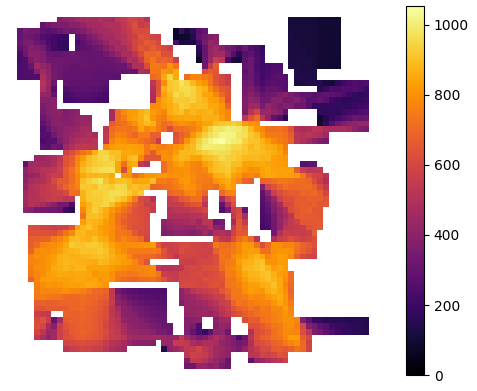
\includegraphics[width=0.45\textwidth]{images/visibility_old.png}}
    \qquad
    \subfloat[The visibility matrix, computed in 0.26s]{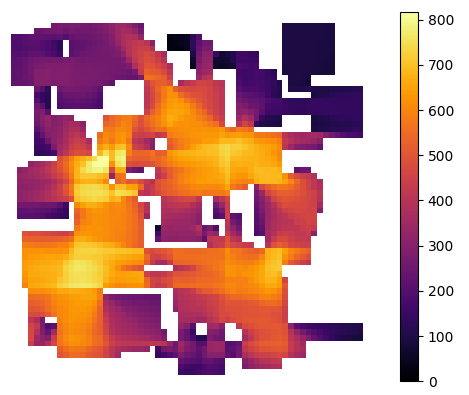
\includegraphics[width=0.45\textwidth]{images/visibility_new.png}}
    \caption[Visibility comparison]{Examples of the visibility matrix obtained with the naive method and the grid-based method. The color of a tile represents the number of tiles visible from it.}
    \label{fig:visibility_example}
\end{figure}

From this visibility matrix we can extract the following \textbf{visibility-based} features:

\begin{itemize}
    \item \textit{maxValueVisibility}: Maximum value of the visibility matrix, which represents the maximum number of tiles visible from a single tile.
    \item \textit{maxValuePercentVisibility}: Maximum value of the visibility matrix divided by the total number of walkable tiles.
    \item \textit{averageLocalMaximaValuePercentVisibility}: The average of the values of all local maxima of the visibility matrix divided by the total number of walkable tiles.
    \item \textit{averageValuePercentVisibility}: The average value of the visibility matrix divided by the total number of walkable tiles.
    \item \textit{quantile25PercentVisibility}: The first quartile of the visibility matrix divided by the total number of walkable tiles.
    \item \textit{quantile50PercentVisibility}: The second quartile (median) of the visibility matrix divided by the total number of walkable tiles.
    \item \textit{quantile75PercentVisibility}: The third quartile of the visibility matrix divided by the total number of walkable tiles.
    \item \textit{stdValuePercentVisibility}: The standard deviation of the values of the visibility matrix divided by the total number of walkable tiles.
    \item \textit{localMaximaNumberVisibility}: The number of local maxima of the visibility matrix.
    \item \textit{localMaximaTopDistanceVisibility}: The distance between the two local maxima with the highest values of the visibility matrix.
    \item \textit{localMaximaAverageDistanceVisibility}: The average distance between all local maxima of the visibility matrix.
    \item \textit{stdLocalMaximaValuePercentVisibility}: The standard deviation of the values of all local maxima of the visibility matrix divided by the total number of walkable tiles.
\end{itemize}

Another particularly interesting topological measure is a map's symmetry. Symmetry is an important concept in level design, both from a balancing perspective and from an aesthetic perspective. We have measured symmetry as the percentage of tiles that are equal to their symmetrical counterpart with respect to the map's center axis, obtaining the following \textbf{symmetry-based} features:

\begin{itemize}
    \item \textit{xSymmetry}: The percentage of tiles that are equal to their symmetrical counterpart with respect to the map's vertical axis.
    \item \textit{ySymmetry}: The percentage of tiles that are equal to their symmetrical counterpart with respect to the map's horizontal axis.
    \item \textit{maxSymmetry}: The maximum value between xSymmetry and ySymmetry.
\end{itemize}

Finally, we have tried to define measures that would describe certain types of maps that could be interesting to illuminate. We have thus defined the following \textbf{aggregate} features:

\begin{itemize}
    \item \textit{balanceTopology}: A measure of how balanced a map's topology is, meaning that rooms are well-connected, loops are present, and rooms are generally well-distributed. It is calculated as follows:
    \begin{equation}
    \begin{split}
        &explorationFactor = clip\left(\dfrac{averageMincut}{2}, 0, 1\right) \\
        &evenlySpacedFactor = 1 - \dfrac{stdRoomMinDistance}{30} \\
        &cyclesFactor = clip\left(\dfrac{numberCyclesTwoRoom}{5}, 0, 1\right) \\
        &balanceTopology = explorationFactor + evenlySpacedFactor \\
        &+ cyclesFactor
    \end{split}
    \end{equation}
    Note that the value "30" in the evenlySpacedFactor is an empirical value from the observed maximum of \textit{stdRoomMinDistance}.
    \item \textit{explorationPlusVisibility}: A measure to describe how much a map encourages exploration by being well-connected and having good visibility. It is calculated as follows:
    \begin{equation}
    \begin{split}
        &explorationFactor = clip\left(\dfrac{averageMincut}{2}, 0, 1\right) \\
        &visibilityFactor = clip\left(localMaximaNumberVisibility, 0, 1\right)\\ 
        &* averageValuePercentVisibility \\
        &explorationPlusVisibility = explorationFactor + visibilityFactor
    \end{split}
    \end{equation}
\end{itemize}

\section{Summary}
In this chapter we have described the already existing genomes \textit{All-Black} and \textit{Grid-Graph}, and the newly defined genomes \textit{Point-Line} and \textit{SMT-Genome}. We have also described the common phenotype \textit{Areas-Phenotype} used to interface the representations with \textit{Project-Arena}. We have then listed and described all the emergent features extracted from simulated gameplay data and all the topological features extracted from the map's topology, using room segmentation to derive a graph representation and graph-based visibility methods to extract the visibility matrix.

\chapter{Experiments}
In this chapter we are going to illuminate the feature space of competitive First-Person Shooter maps using a Quality Diversity algorithm.

First, we run some preliminary analysis to understand the noisiness of the simulation-based features and the noisiness of the features extracted from the \textit{SMT-Genome} representation, whose phenotype mapping is not deterministic.

Then we will run a correlation analysis to understand how features correlate with one another, so that we can identify patterns and group features that are highly correlated and reduce the number of features to be examined. We will then look for interesting couples of features that are negatively correlated, as these could be interesting to explore using a QD approach.

Finally, we will use \textit{t-SNE} to visualize the high-dimensional feature space of the maps, the space of the map's images defined by their tiles grid and the space of the map's graph, encoded using a graph embedding method. We will then compare the clustering of the maps in these spaces to understand how features correlate with the visual appearance of the maps and with their topological structure as described by the graph. We will also analyze how the maps' distance in the space projected by \textit{t-SNE} correlates with their features.

Finally, we leverage the insights gained from these analyses to identify three \textit{behavioral characterizations} by selecting relevant couples of features to be illuminated using the \textit{Map-Elites with Sliding Boundaries} algorithm, with the goal of producing maps where gameplay is balanced between bots of differing skill levels. We will then compare the results obtained using different genome representations to understand the differences in their capability to generate varied and balanced designs.

\section{Preliminary analysis}
\subsection{Emergent features noisiness analysis}
\label{subsec:emergent_features_noisiness}
By their very nature, simulations are not deterministic given that bots perform many random actions during a single match. So, while topological features are always the same for a given map, emergent features, such as entropy or pace, may vary. For this reason, we have run an analysis to understand how noisy these features are; if a feature varies too wildly between different matches on the same map, then we may as well consider it random and unfit to describe an actual feature of the examined map.

To gather and visualize this data we have generated a random genome (one for all genome representations discussed in \cref{sec:map_genomes}), converted it to a phenotype and run 100 different matches on the same map, recording the emergent features at the end of each match. Each feature has thus 100 data points which have been used to draw a boxplot\footnote{\url{https://pandas.pydata.org/docs/reference/api/pandas.DataFrame.boxplot.html}}, which allows us to neatly visualize the distribution (median, first and third quartile, maximum, minimum and outliers) of the data. While some features, such as entropy or pace, have a maximum and minimum possible value, others, such as the maximum value of the heatmaps, do not. In order to visualize and compare features we have normalized all features to the range $[0, 1]$, using the empirical minimum and maximum values, obtained from roughly 16000 matches on different maps, when needed. The results are shown in figures \cref{fig:emergent_features_noisiness_ab}, \cref{fig:emergent_features_noisiness_grid}, \cref{fig:emergent_features_noisiness_pointad} and \cref{fig:emergent_features_noisiness_smt}.

\begin{figure}[p]
    \centering
    \subfloat{

        
\includegraphics[width=0.15\textwidth, valign=c]{images/phenotype_var_ab_0_nm1.png}
        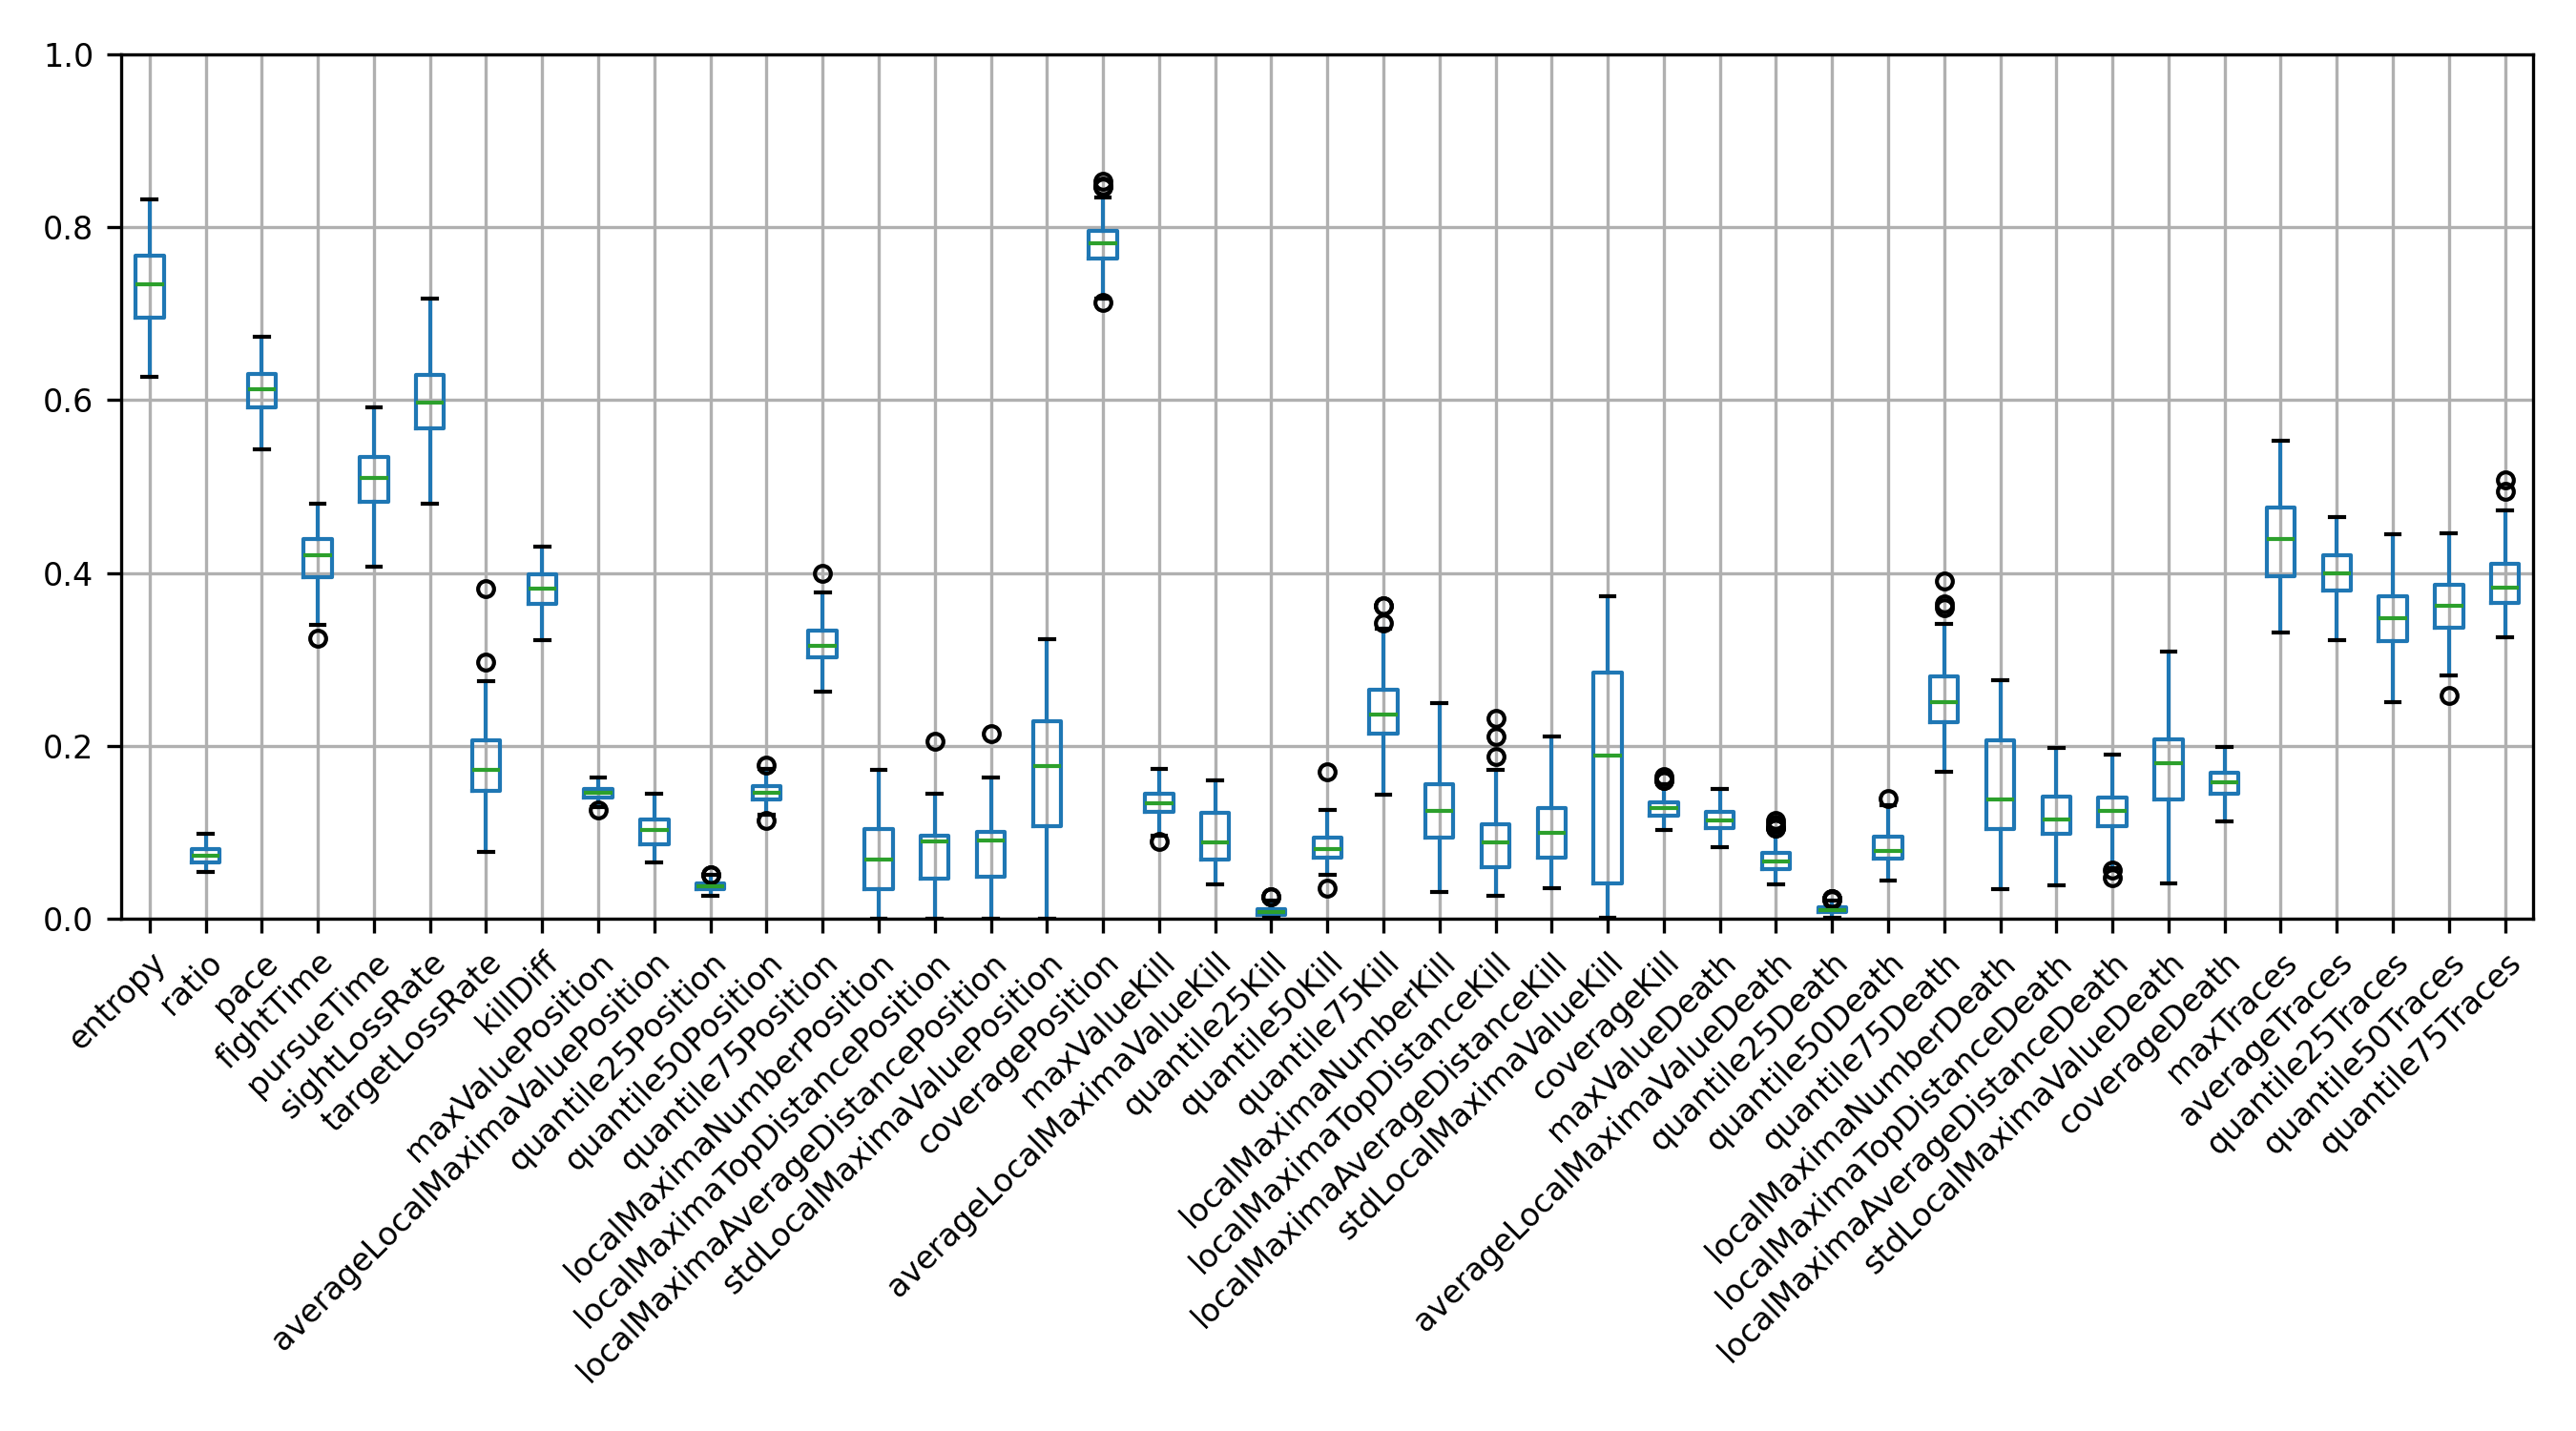
\includegraphics[width=0.85\textwidth, valign=c]{images/boxplot_var_ab_0_nm1_numsim_1.png}
        }
    \caption{Boxplot of emergent features for a random \textit{All-Black} phenotype.}
    \label{fig:emergent_features_noisiness_ab}
\end{figure}
\begin{figure}[p]
    \centering
    \subfloat{
        
\includegraphics[width=0.15\textwidth, valign=c]{images/phenotype_var_grid_0_nm1.png}
        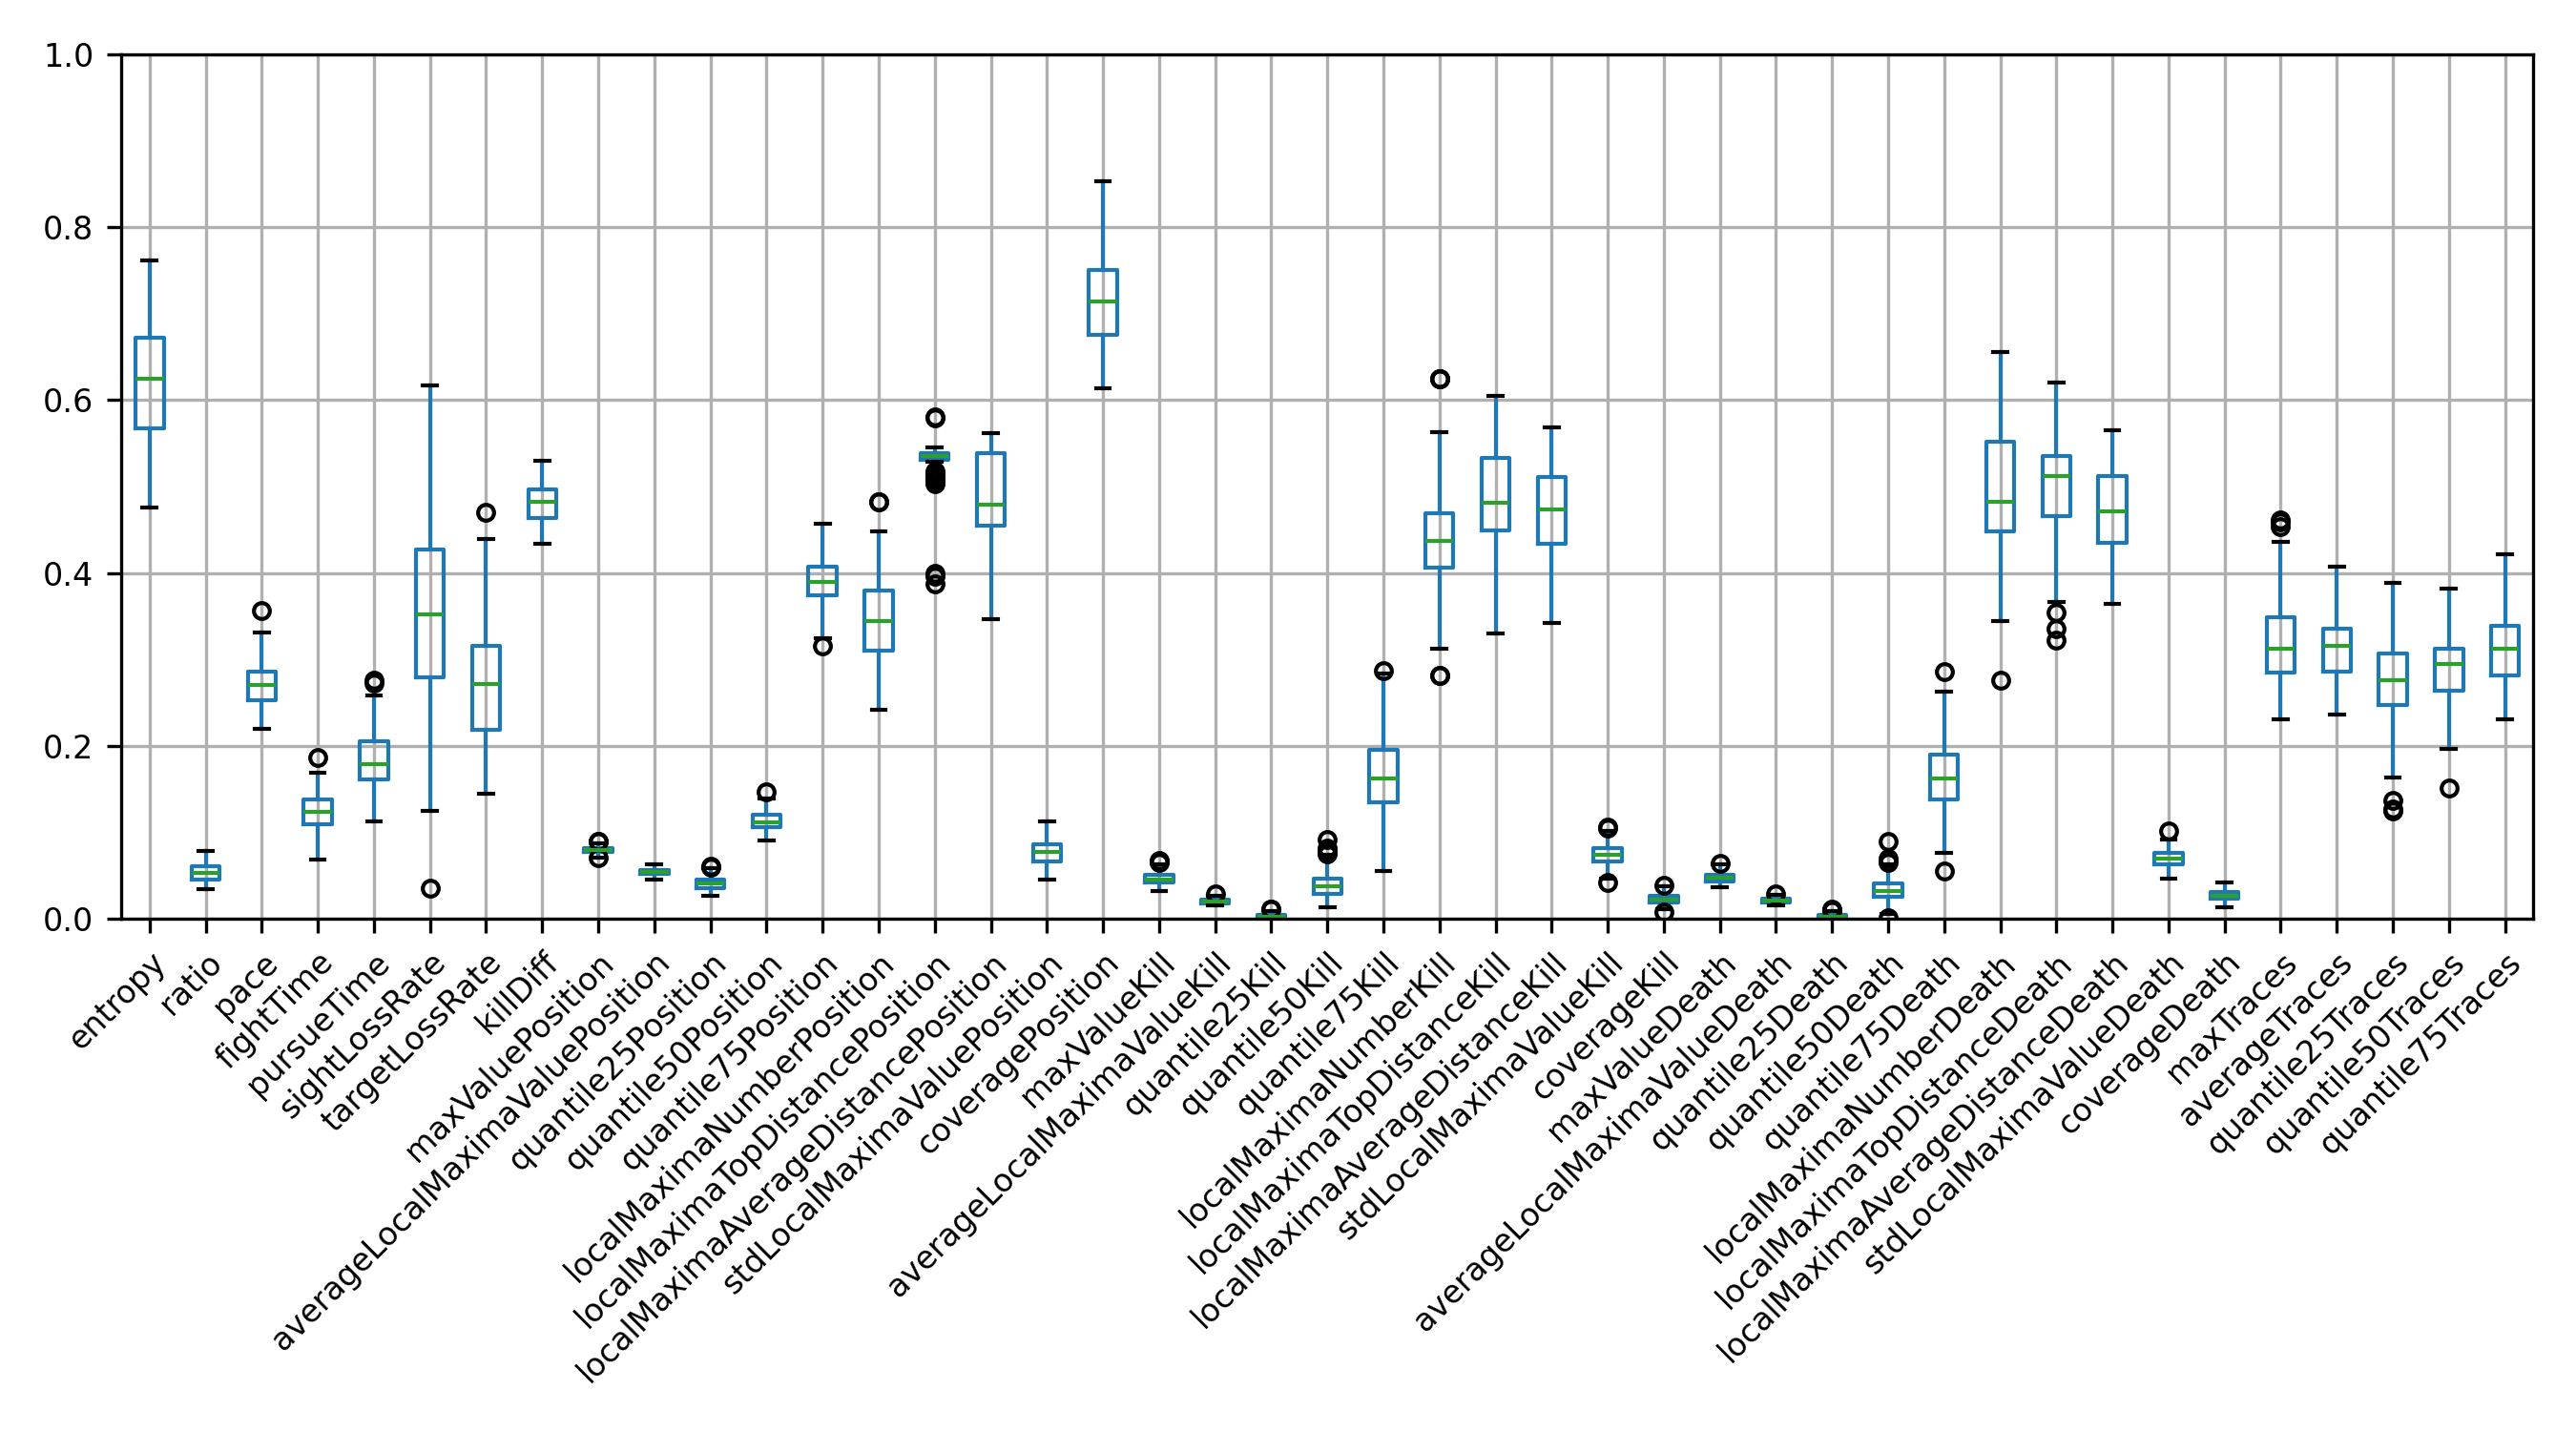
\includegraphics[width=0.85\textwidth, valign=c]{images/boxplot_var_grid_0_nm1_numsim_1.png}
        }
    \caption{Boxplot of emergent features for a random \textit{Grid-Graph} phenotype.}
    \label{fig:emergent_features_noisiness_grid}
\end{figure}
\begin{figure}[p]
    \centering
    \subfloat{
        
\includegraphics[width=0.15\textwidth, valign=c]{images/phenotype_var_pointad_0_nm1.png}
        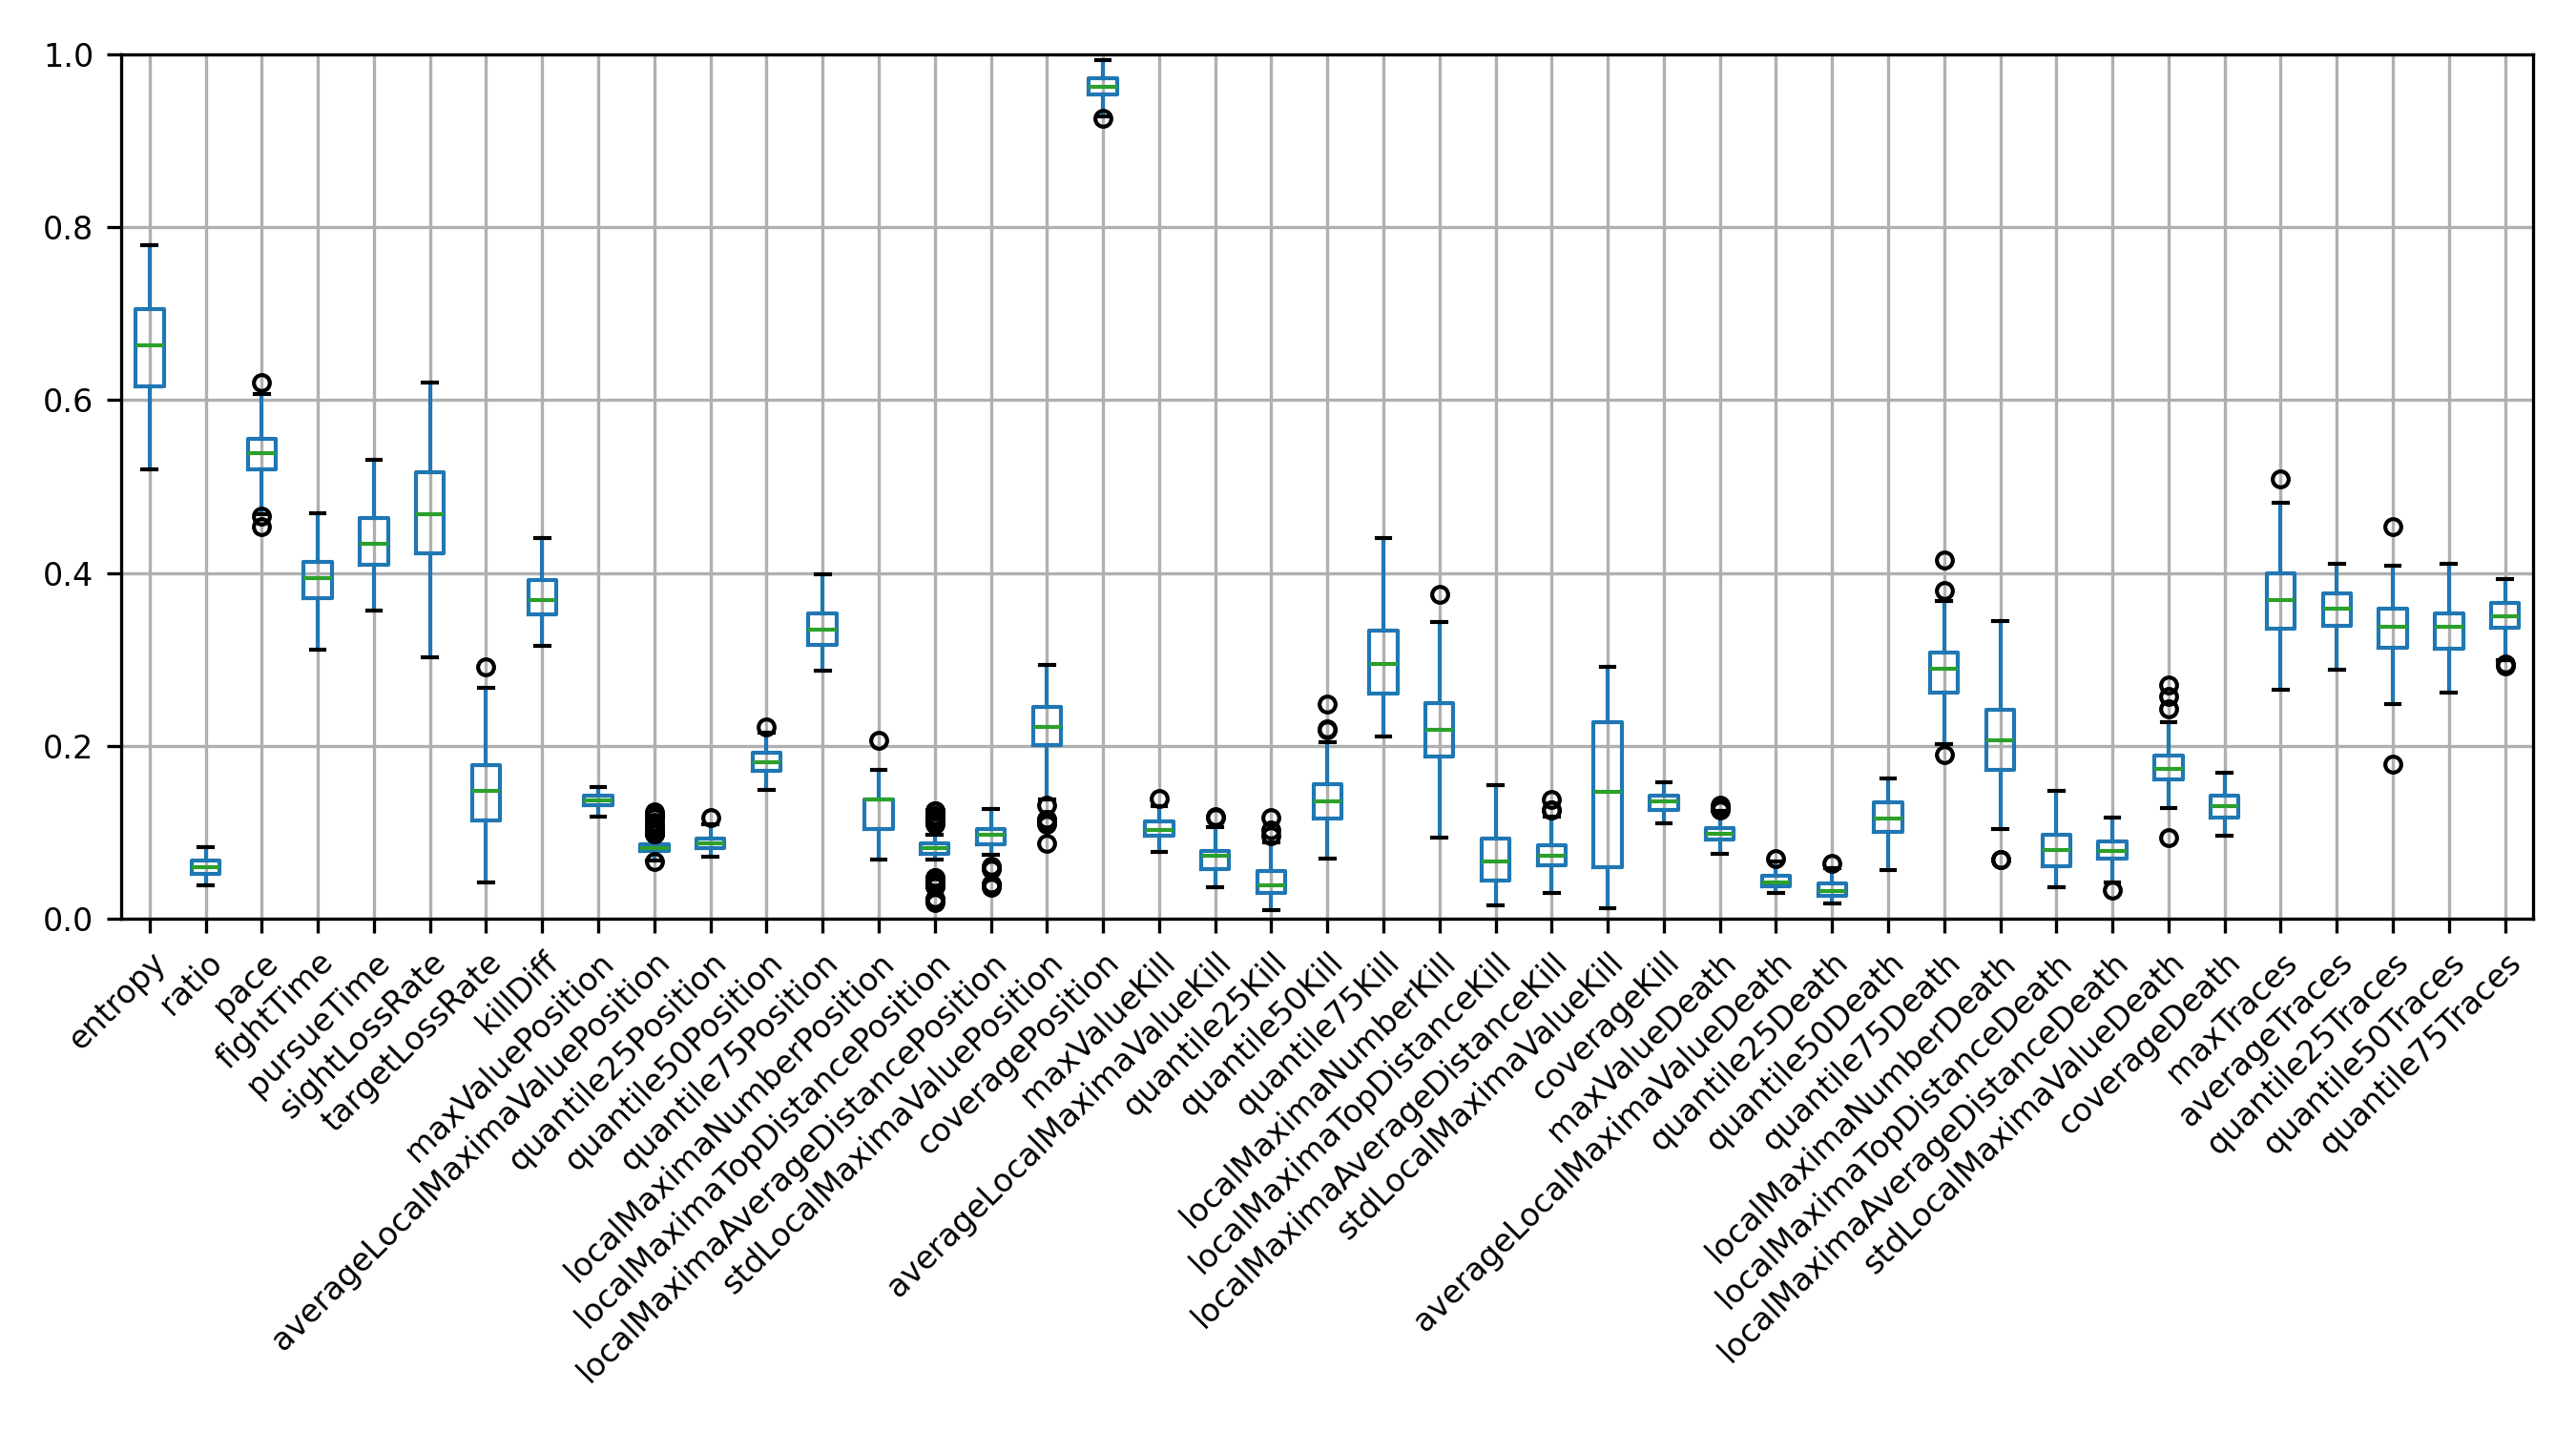
\includegraphics[width=0.85\textwidth, valign=c]{images/boxplot_var_pointad_0_nm1_numsim_1.png}
    }
    \caption{Boxplot of emergent features for a random Point-Line phenotype.}
    \label{fig:emergent_features_noisiness_pointad}
\end{figure}
\begin{figure}[p]
    \centering
    \subfloat{
        
        
\includegraphics[width=0.15\textwidth, valign=c]{images/phenotype_var_smt_0_nm1.png}
        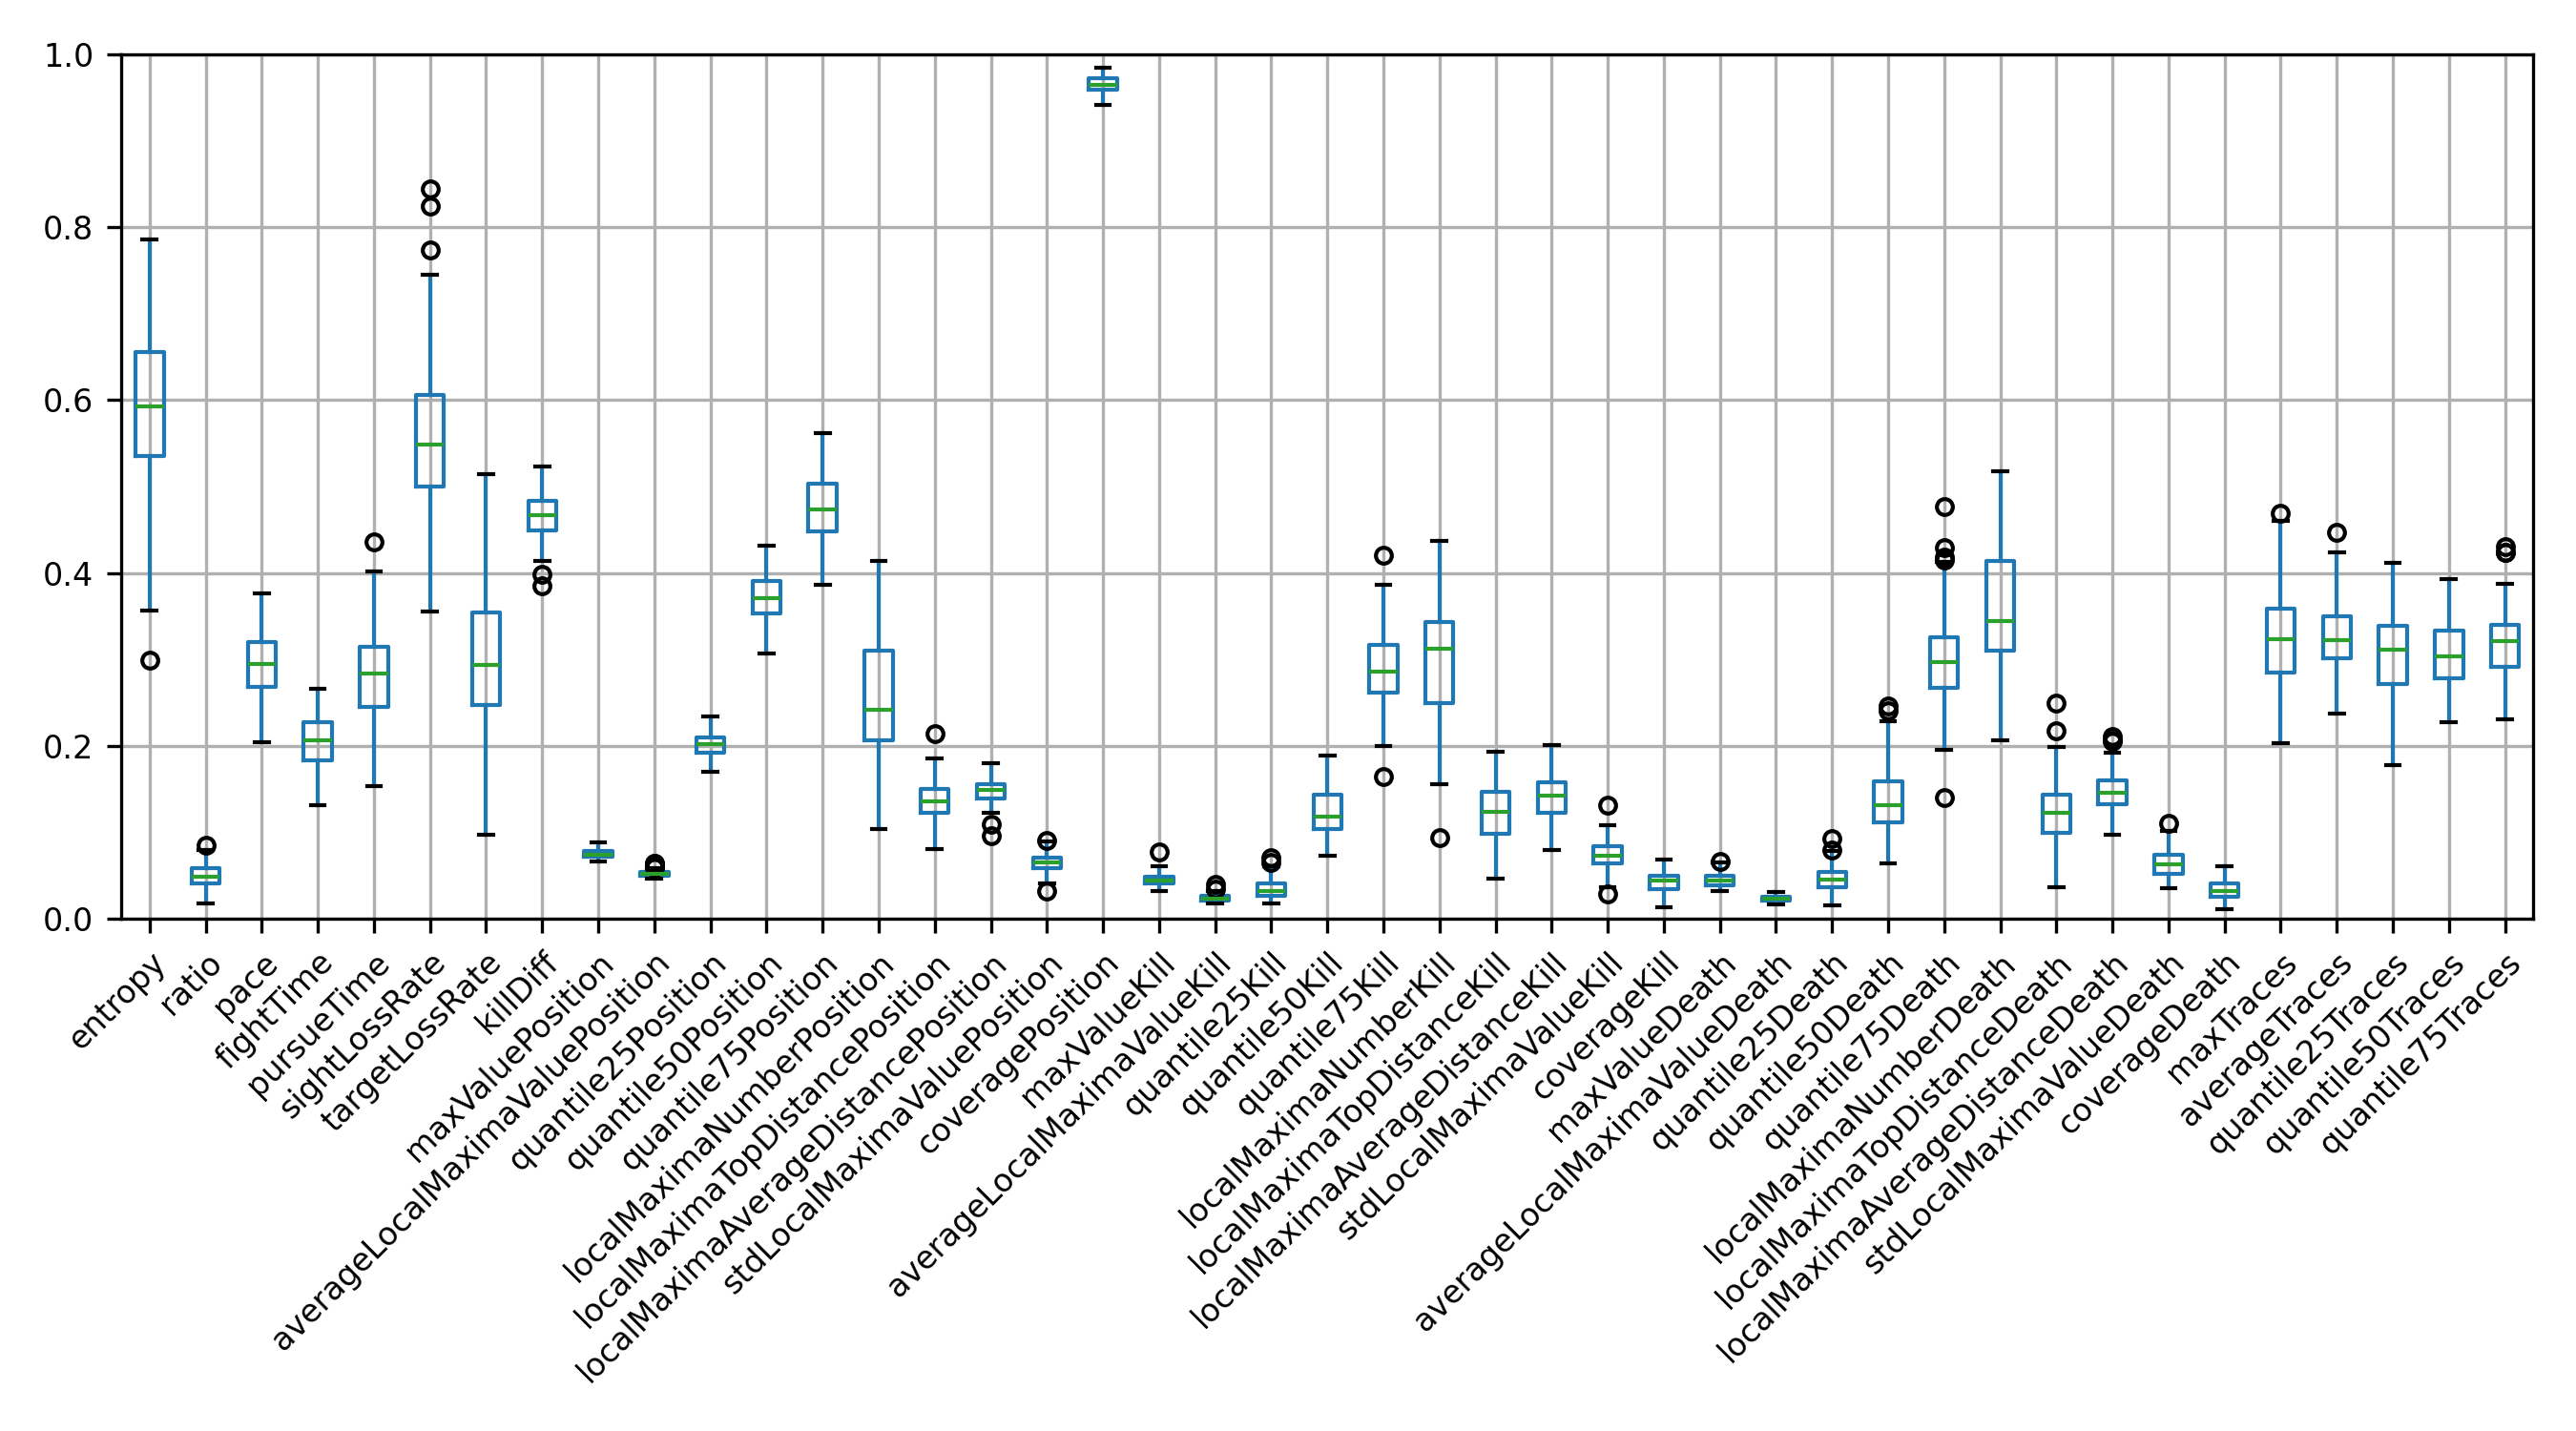
\includegraphics[width=0.85\textwidth, valign=c]{images/boxplot_var_smt_0_nm1_numsim_1.png}
    }
    \caption{Boxplot of emergent features for a random SMT phenotype.}
    \label{fig:emergent_features_noisiness_smt}
\end{figure}

\clearpage
We notice that results do not differ significantly between different genomes. We can also conclude that, while some features are occasionally noisier (e.g. stdLocalMaximaValueKill in \cref{fig:emergent_features_noisiness_ab}, sightLossRate in \cref{fig:emergent_features_noisiness_grid} and entropy in \cref{fig:emergent_features_noisiness_smt}), in general all have a reasonable and similar amount of noise. To improve our results, we believe that averaging the features over multiple matches would be beneficial. To this end, we repeated the analysis by averaging the features over 5 matches, obtaining again 100 data points for each feature, where each data point is the average of the result of 5 matches. The results are shown in figures \cref{fig:emergent_features_noisiness_5_ab}, \cref{fig:emergent_features_noisiness_5_grid}, \cref{fig:emergent_features_noisiness_5_pointad} and \cref{fig:emergent_features_noisiness_5_smt}.

\vspace*{\fill}
{
\centering
\begin{figure}[hbt!]
    \centering
    \subfloat{ 
        \centering
        
\includegraphics[width=0.15\textwidth, valign=c]{images/phenotype_var_ab_0_nm5.png}
        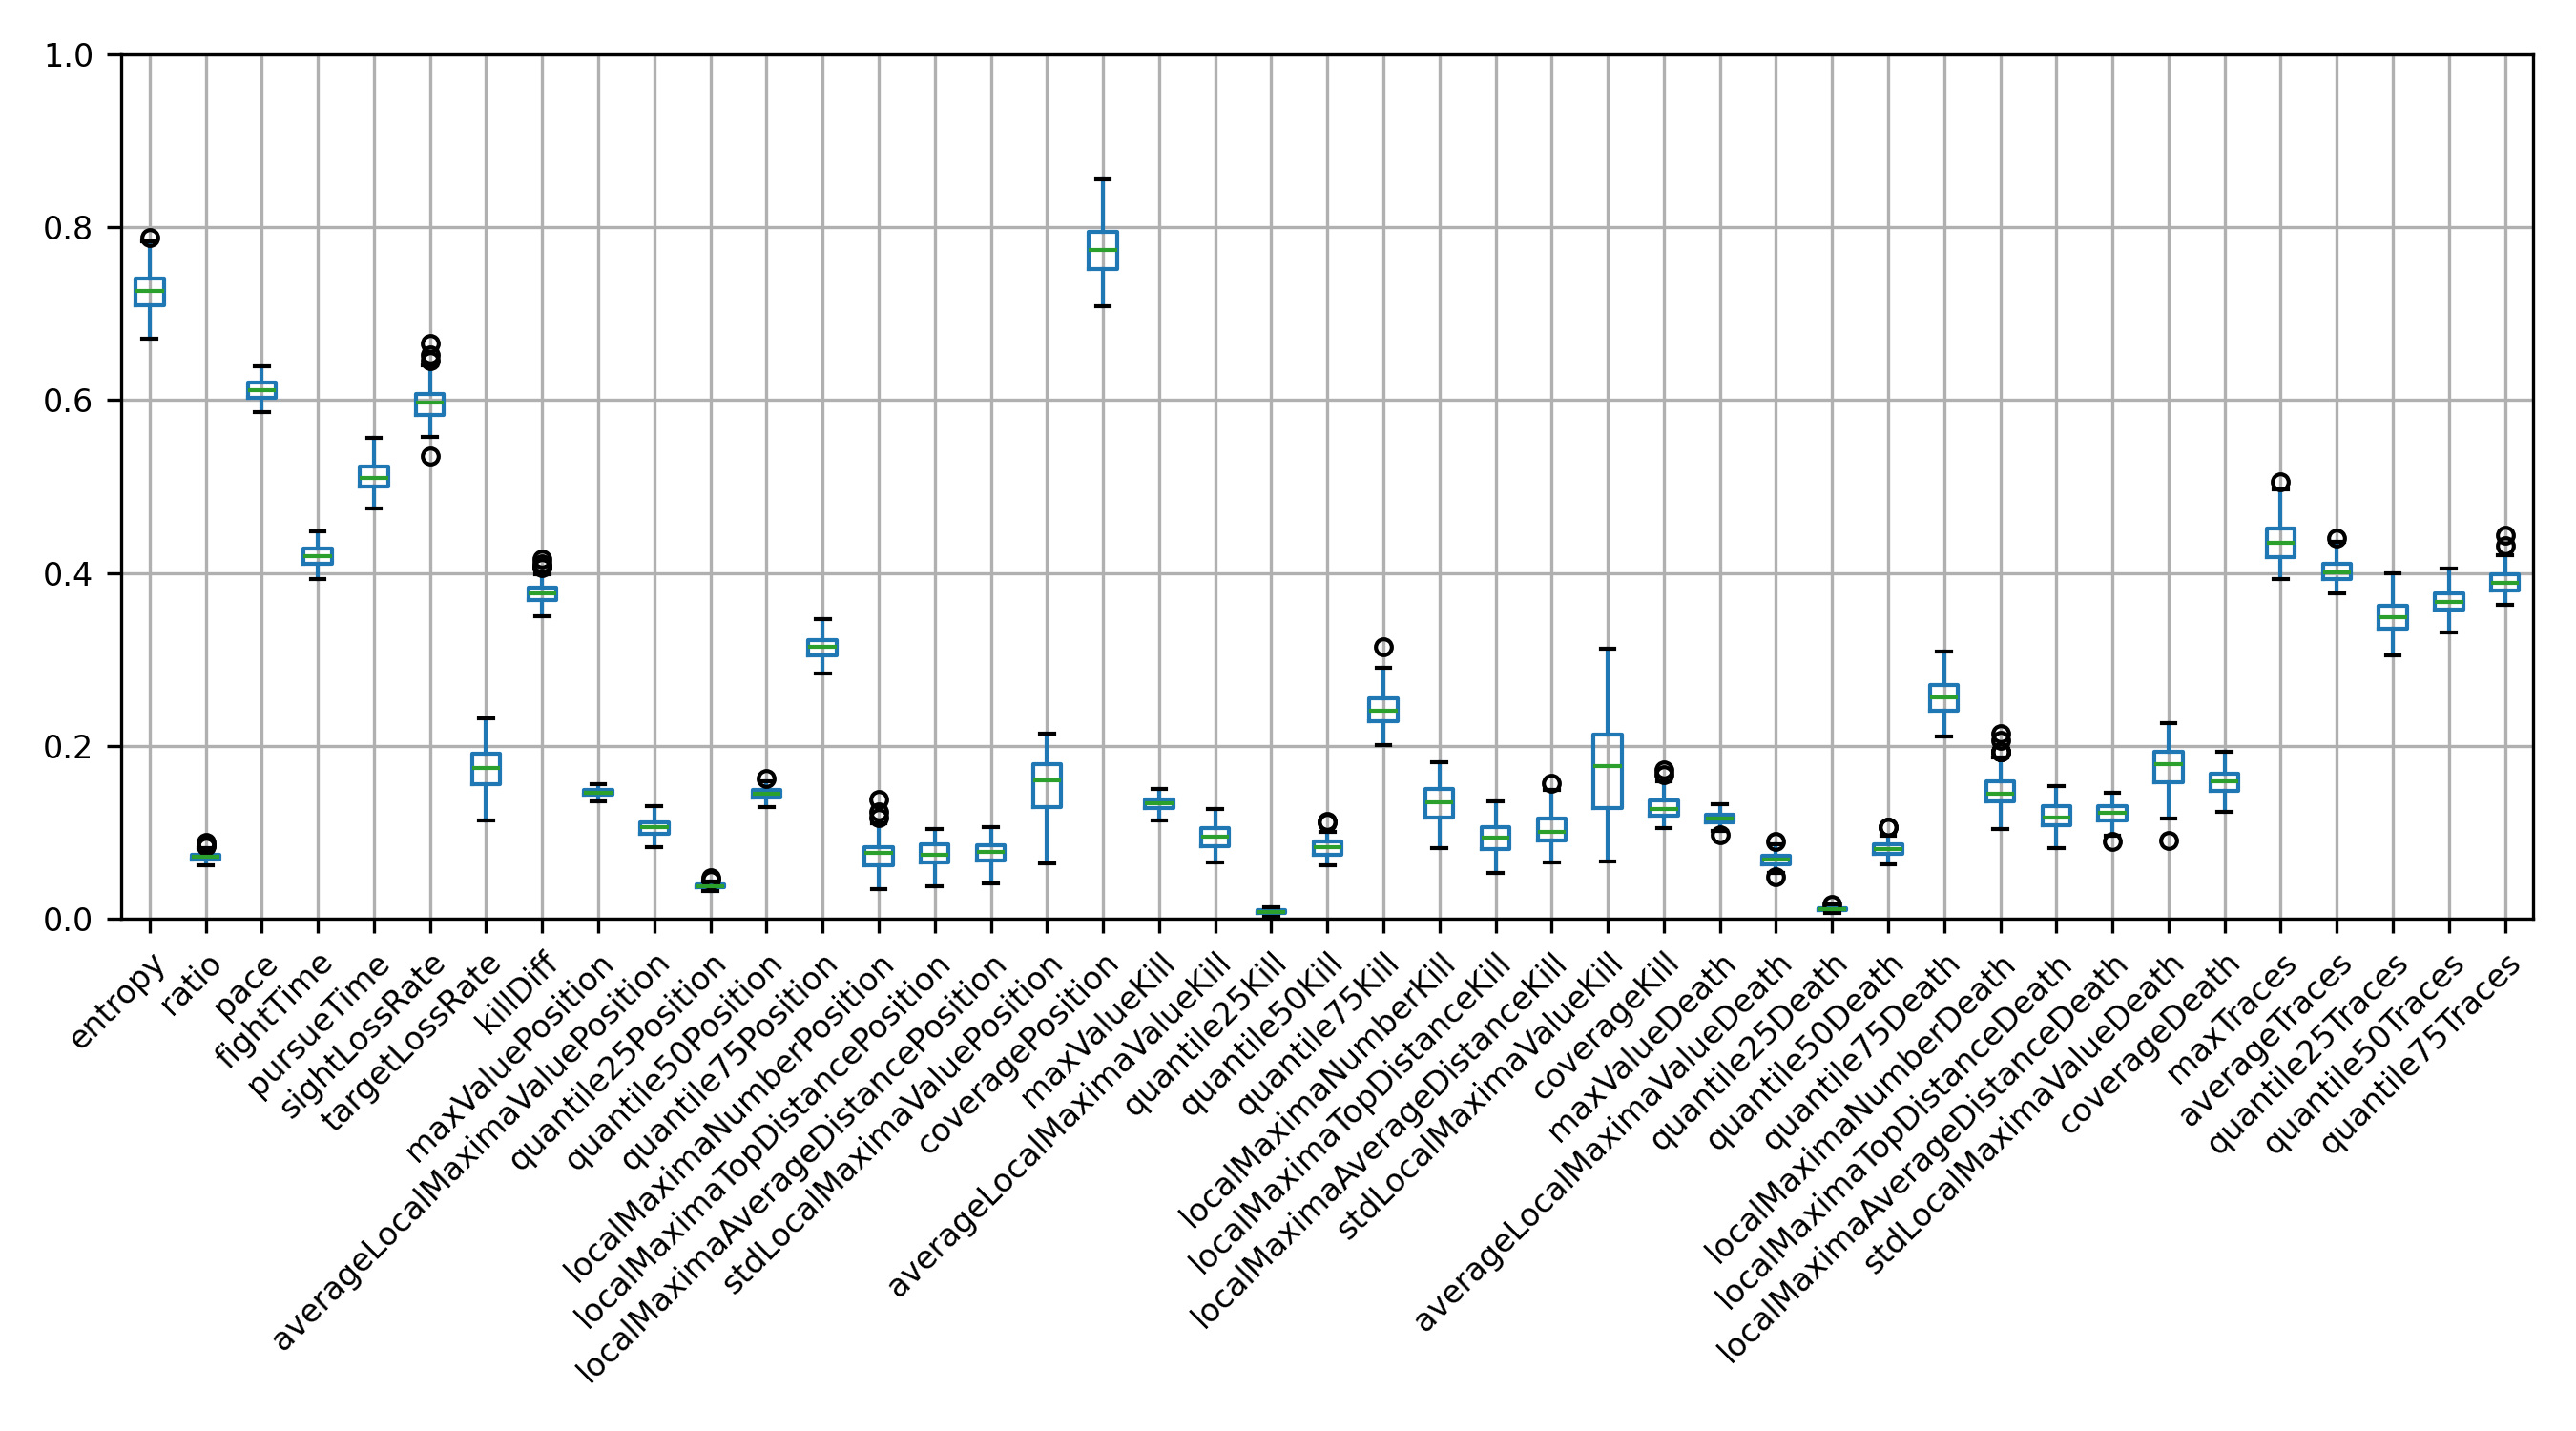
\includegraphics[width=0.85\textwidth, valign=c]{images/boxplot_var_ab_0_nm5_numsim_5.png}
    }
    \caption{Boxplot of emergent features for a random \textit{All-Black} phenotype averaging 5 matches.}
    \label{fig:emergent_features_noisiness_5_ab}
\end{figure}
}
\vspace*{\fill}
\begin{figure}[p]
    \subfloat{ 
        \centering
        
\includegraphics[width=0.15\textwidth, valign=c]{images/phenotype_var_grid_0_nm5.png}
        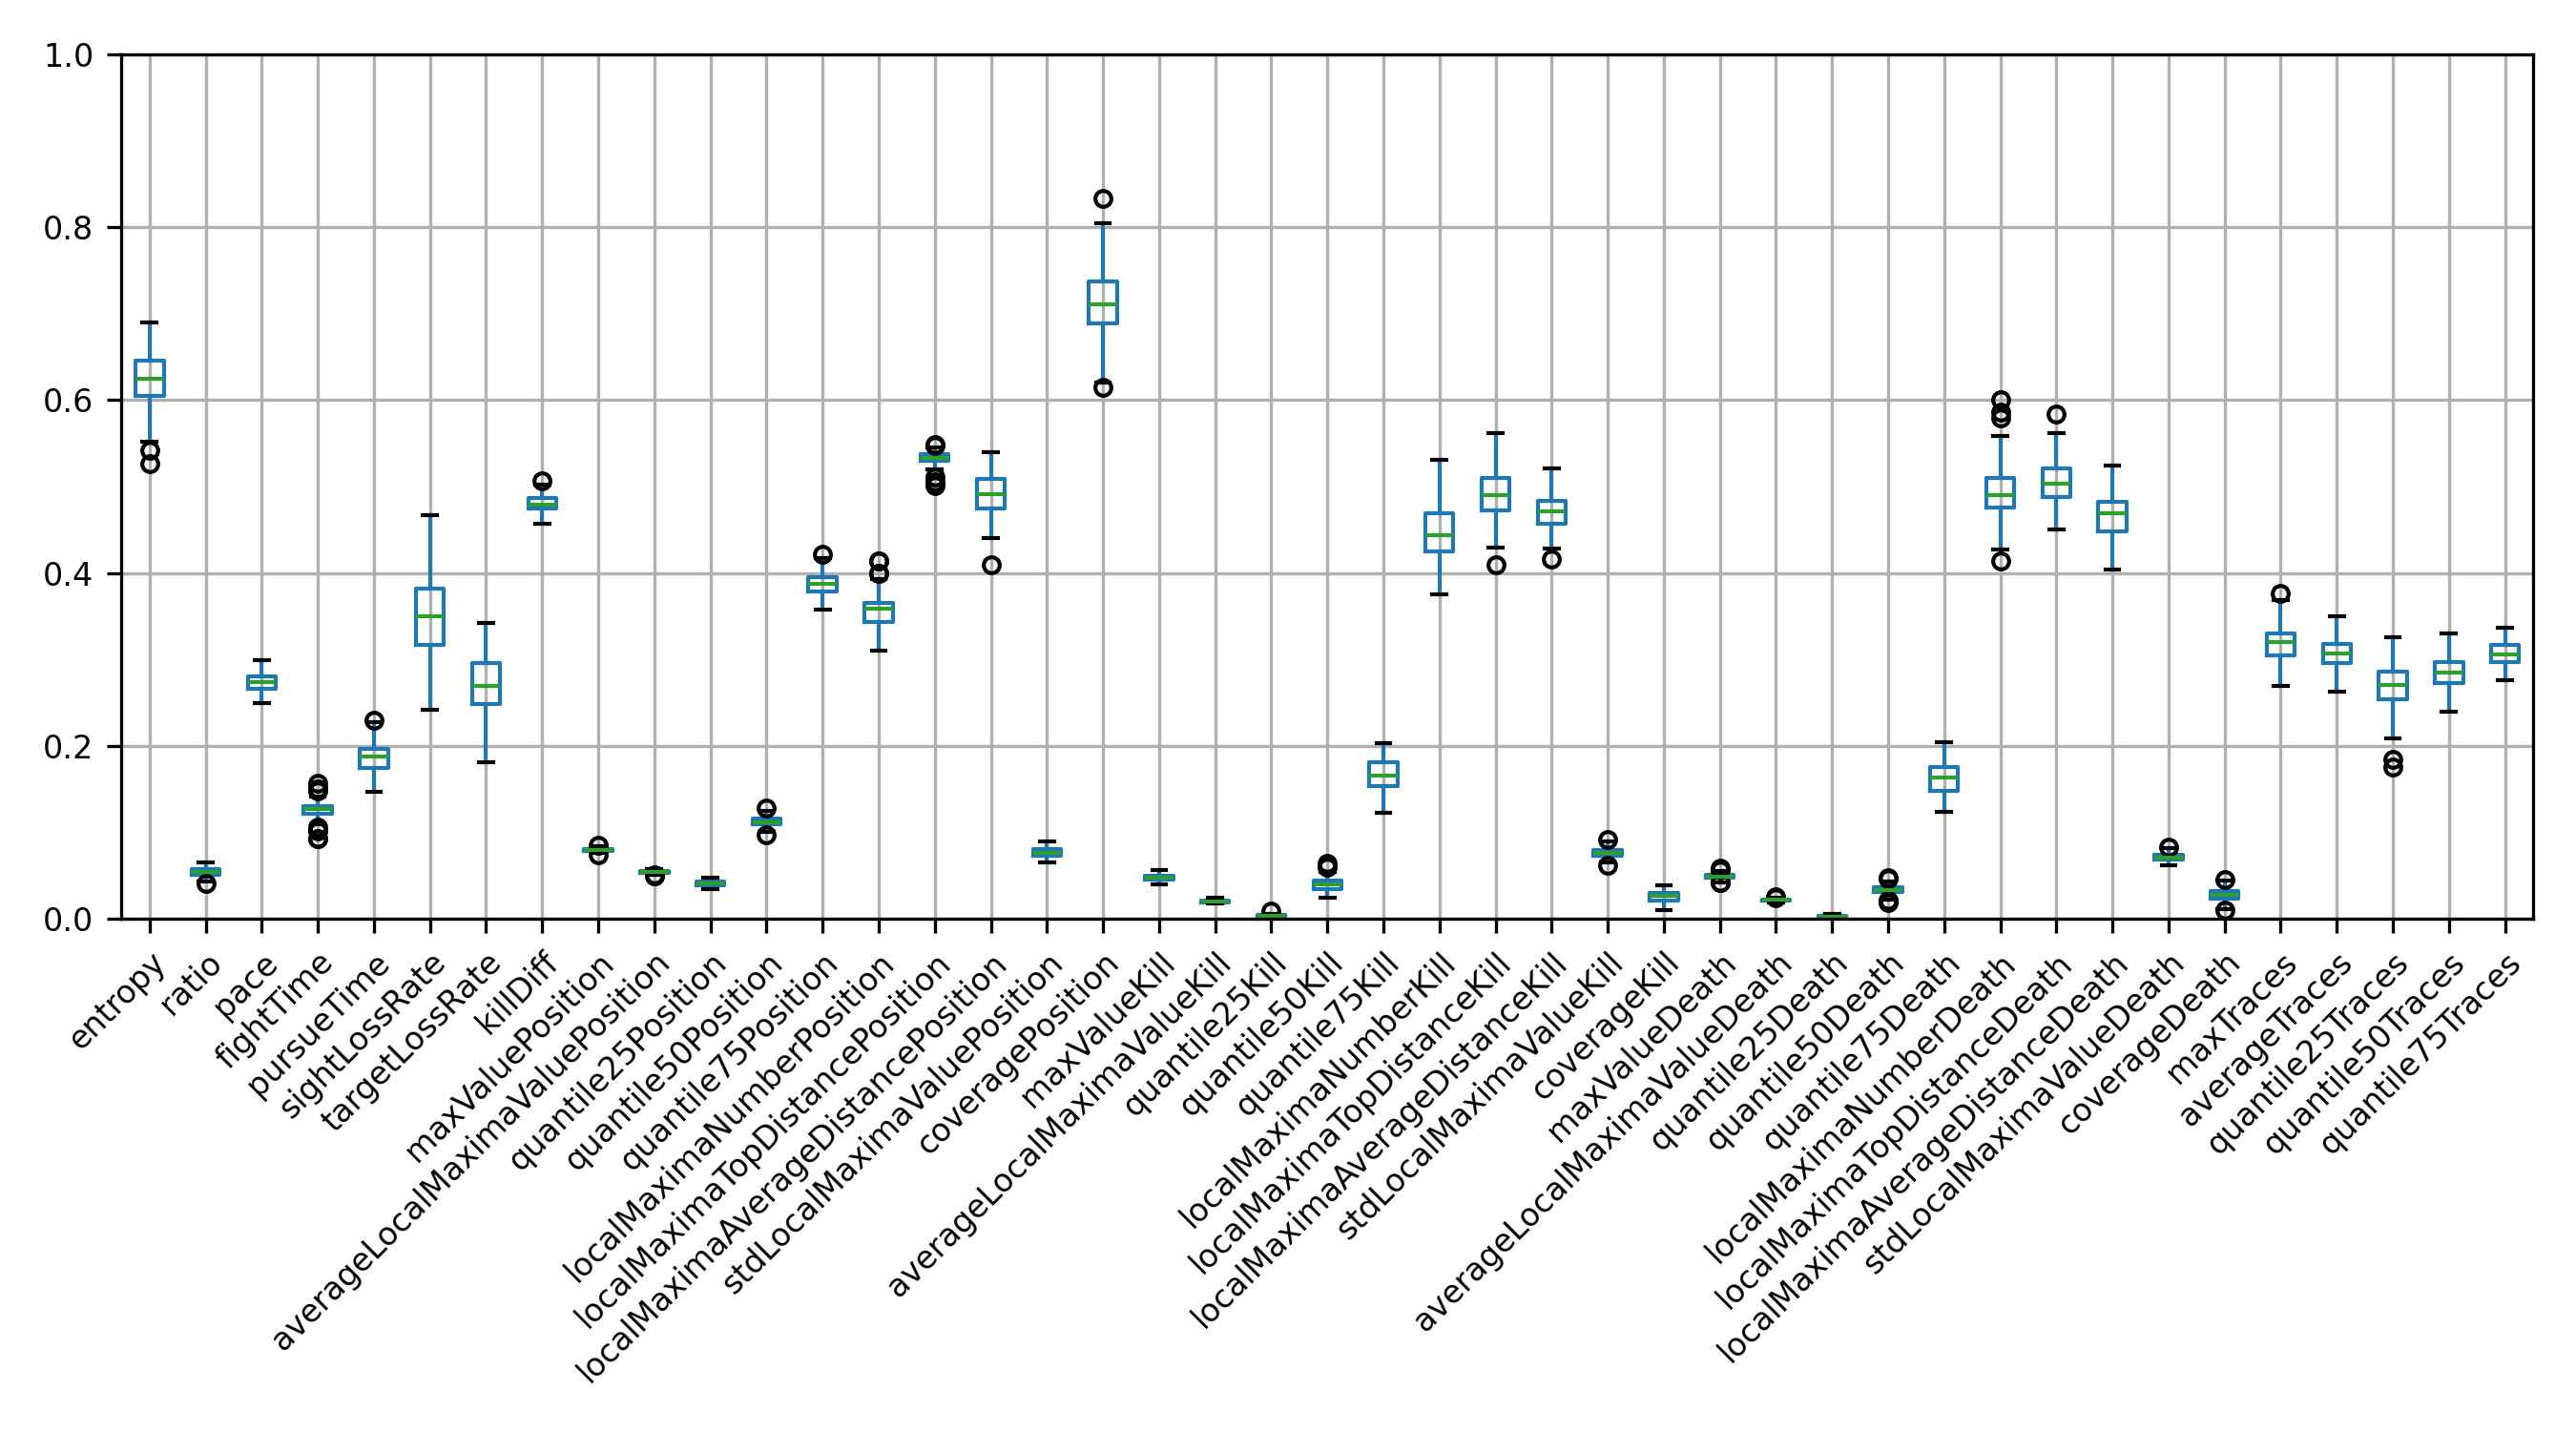
\includegraphics[width=0.85\textwidth, valign=c]{images/boxplot_var_grid_0_nm5_numsim_5.png}
        }
    \caption{Boxplot of emergent features for a random \textit{Grid-Graph} phenotype averaging 5 matches.}
    \label{fig:emergent_features_noisiness_5_grid}
\end{figure}

\begin{figure}[p]
    \subfloat{
        \centering
        
\includegraphics[width=0.15\textwidth, valign=c]{images/phenotype_var_pointad_0_nm5.png}
        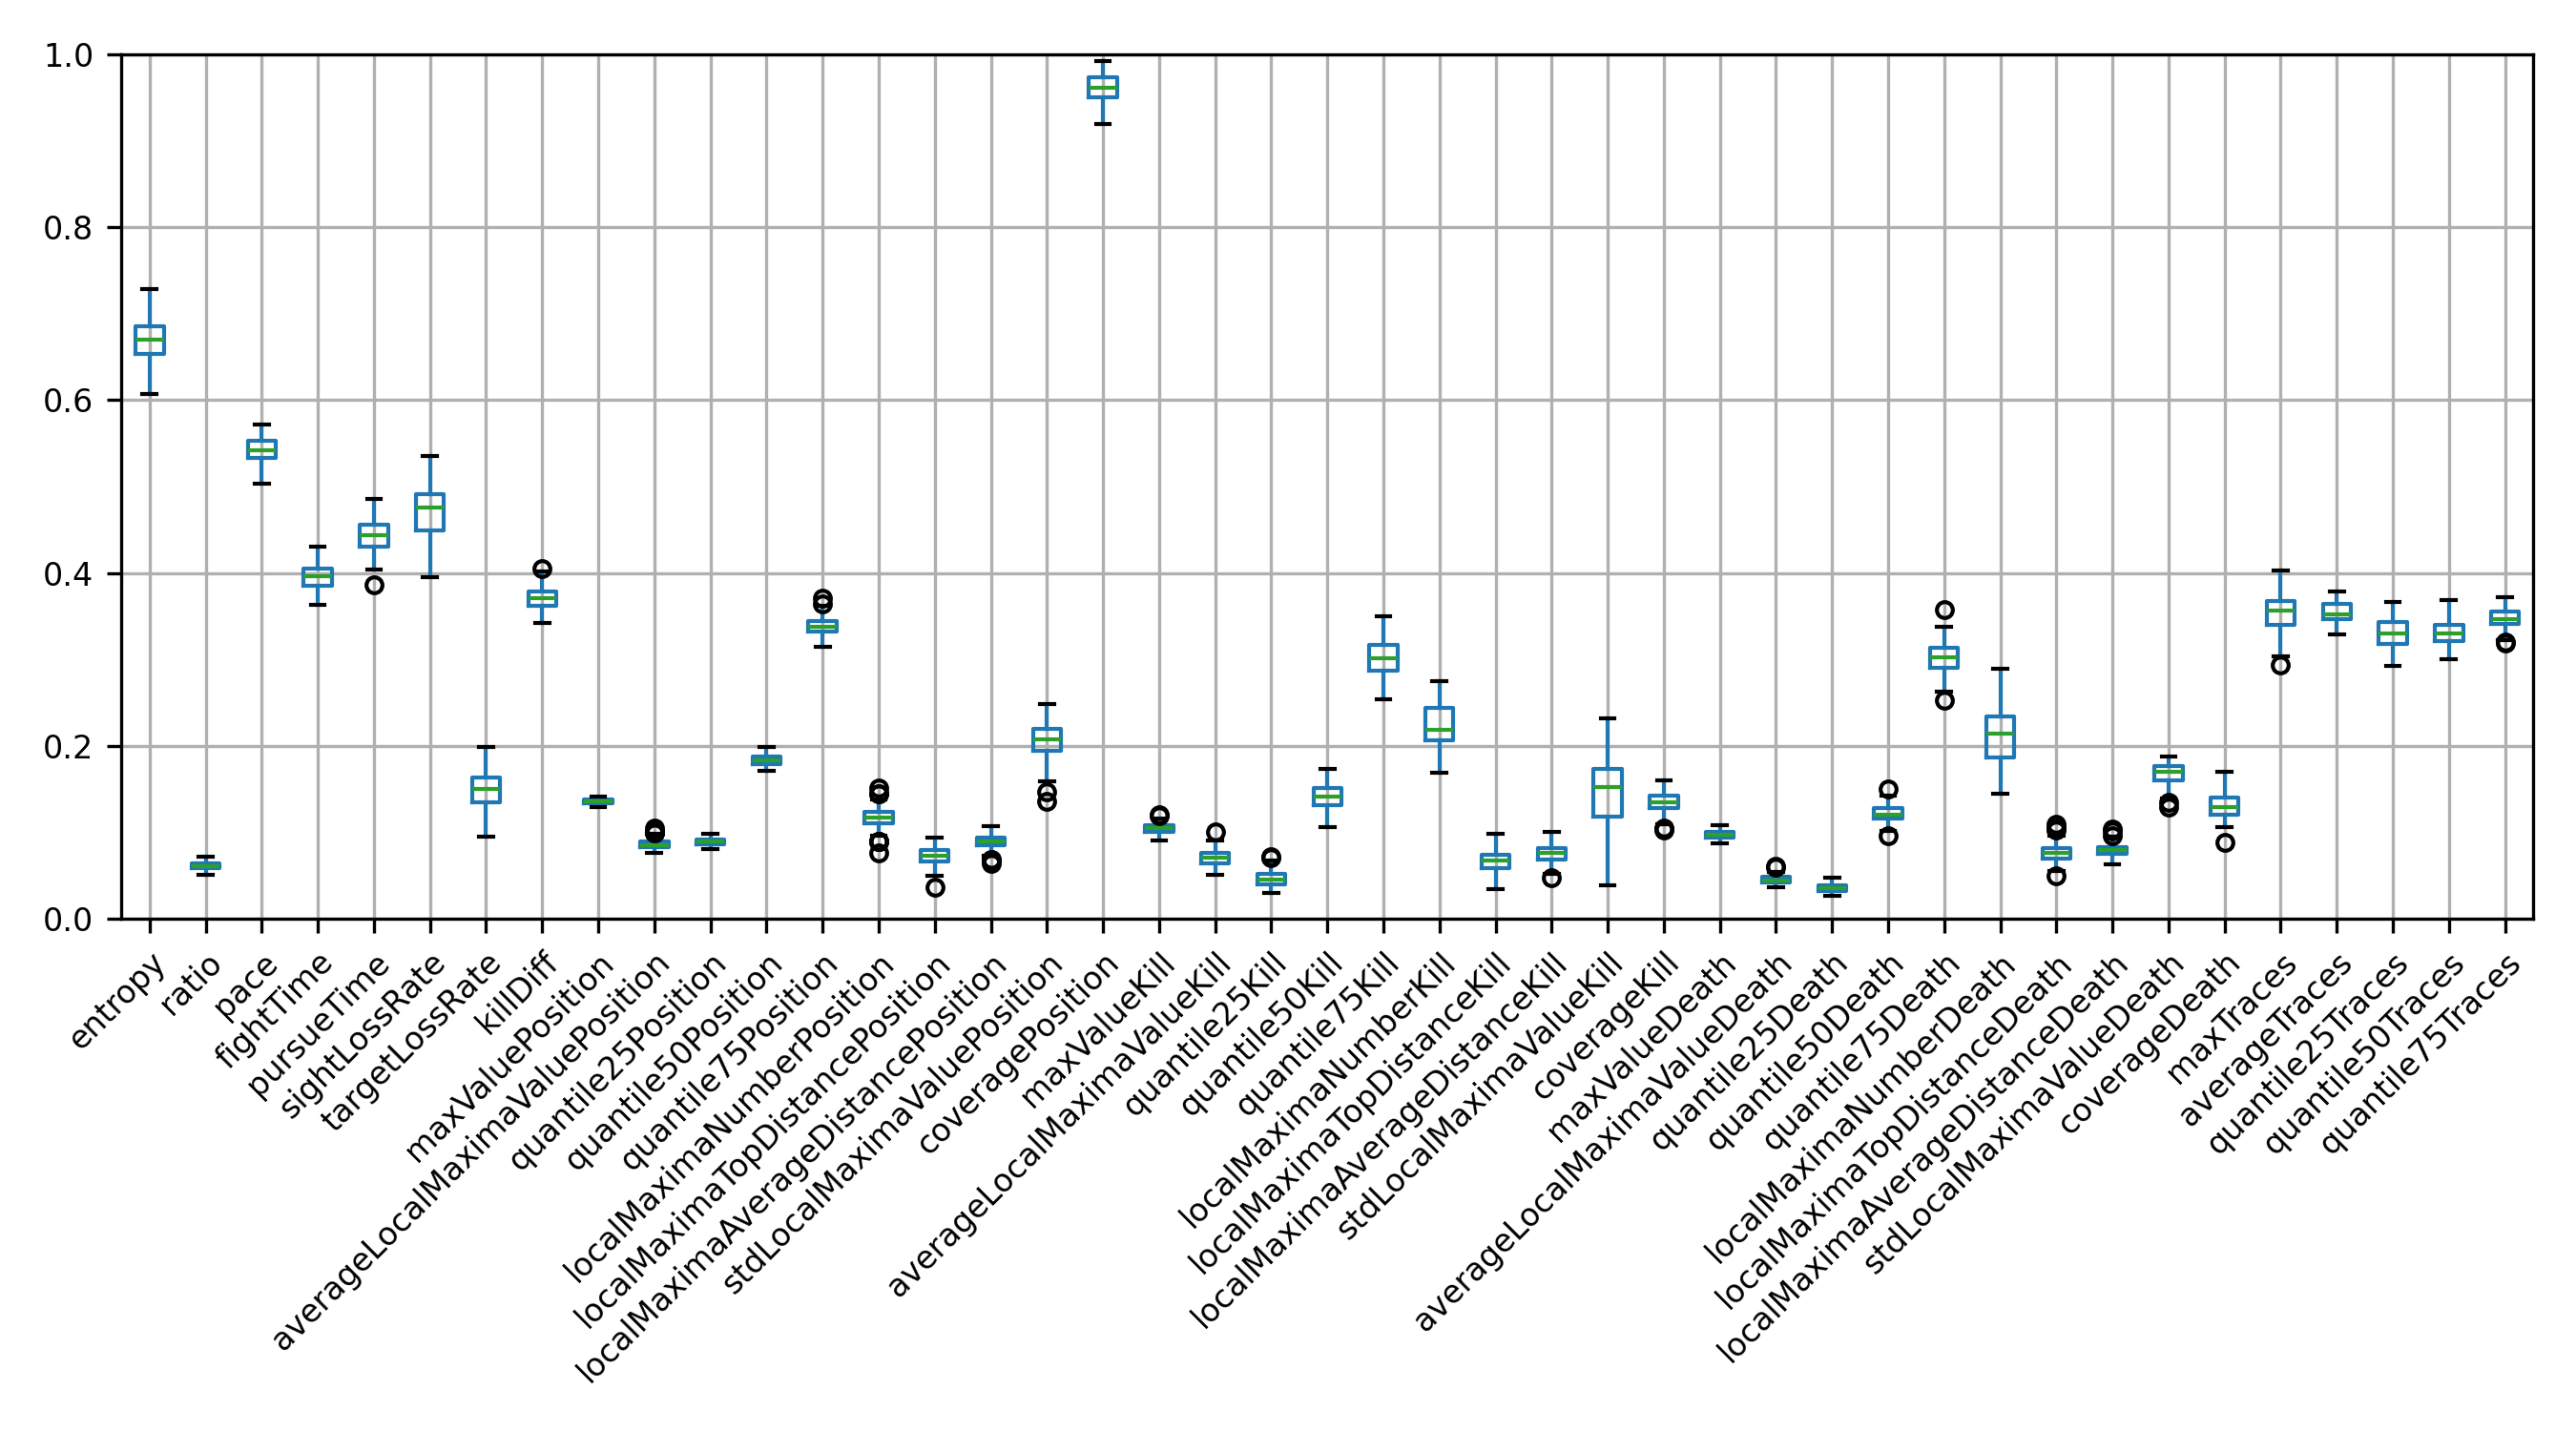
\includegraphics[width=0.85\textwidth, valign=c]{images/boxplot_var_pointad_0_nm5_numsim_5.png}
    }
    \caption{Boxplot of emergent features for a random Point-Line phenotype averaging 5 matches.}
    \label{fig:emergent_features_noisiness_5_pointad}
\end{figure}
\begin{figure}[H]
    \subfloat{ 
        \centering
        
\includegraphics[width=0.15\textwidth, valign=c]{images/phenotype_var_smt_0_nm5.png}
        \includegraphics[width=0.85\textwidth, valign=c]{images/boxplot_var_smt_0_nm5_numsim_5.png}
    }
    \caption{Boxplot of emergent features for a random SMT phenotype averaging 5 matches.}
    \label{fig:emergent_features_noisiness_5_smt}
\end{figure}


As expected, the results are even less noisy, and suggest that all metrics are suitable to describe maps. 

\subsection{SMT-Genome phenotype mapping analysis}
\label{subsec:smt_genome_phenotype_mapping}
As we highlighted in \cref{subsec:smt_genome}, the SMT-Genome is not deterministic, meaning that the same genome could lead to different map layouts when mapped to a phenotype. In this section we determine the noisiness of an SMT-Genome by generating 200 phenotypes from the same genome and calculating both emergent and topological features by simulating 5 matches and averaging results. The 200 data-points are used to draw a boxplot for each feature, which is shown in figures \cref{fig:smt_genome_noisiness_emergent} and \cref{fig:smt_genome_noisiness_topology}.

\begin{figure}[hbt!]
    \centering
    \subfloat{
        \includegraphics[width=0.85\textwidth]{images/boxplot_emergent_smtnoise_f_run2_numsim_5.png}
        }
    \caption{SMT-Genome emergent features noisiness analysis.}
    \label{fig:smt_genome_noisiness_emergent}
\end{figure}
\begin{figure}[hbt!]
    \centering
    \subfloat{
        \includegraphics[width=0.85\textwidth]{images/boxplot_topology_smtnoise_f_run2_numsim_5.png}
    }
    \caption{SMT-Genome topological features noisiness analysis.}
    \label{fig:smt_genome_noisiness_topology}
\end{figure}

For the emergent features in figure \cref{fig:smt_genome_noisiness_emergent} we can clearly see that some features are very noisy, such as entropy, pace, sightLossRate and targetLossRate. For the topological features in figure \cref{fig:smt_genome_noisiness_topology} we can see that the features relating to the cycles are especially noisy, this is probably a consequence of the process of adding connections between rooms based on the lines in the genome, as described in \cref{subsec:smt_genome}, which relies on the intersection between lines and rooms, so often moving the room by a single tile can lead to the room not intersecting a line and thus to a completely different graph. This leads us to believe that the \textit{SMT-Genome} sports very little locality which may impact the evolution process negatively.

\section{Correlation analysis}
\label{sec:correlation_analysis}
Given the considerable number of features that can be extracted from a single map, it would be unfeasible to  try and illuminate all of them. Instead, we examined the correlations of the features with the aim of discovering relevant groups of highly correlated features, which could serve as a basis to explore with a QD method. Knowing how features correlate with one another will give us insights in how exploring a certain feature may affect others and will also help us in exploring interesting areas of the feature space by illuminating couples of features which are negatively correlated.

We generated 100 random genomes and simulated 5 matches on each map, averaging the features obtained in those matches. We used these 100 data points to compute the correlation matrix of the features using Pearson's correlation coefficient\footnote{Correlation coefficient which measures the linear correlation between two sets of data. Its value range from -1 (perfect negative correlation) to 1 (perfect positive correlation), with 0 indicating no correlation.}. We repeated this process for each of the four genome representations, obtaining one correlation matrix for each representation. In order to visualize the data more easily, we averaged the coefficients of these four matrices, obtaining the correlation matrix shown in figure \cref{fig:correlation_matrix_full}.

\begin{figure}[hbt!]
    \centering
    \includegraphics[width=1.0\textwidth]{images/covariance_map_full.png}
    \caption{Correlation matrix of the features.}
    \label{fig:correlation_matrix_full}
\end{figure}

It is immediately apparent that multiple features are not only highly correlated, as highlighted by the white squares on the diagonal, but also that they have similar correlation values with all other features, since multiple consecutive rows show similar values for all cells. Features are ordered on the axis "semantically", meaning that features that are conceptually similar are close to each other. Thus, we first group features by selecting only one feature from each group of highly correlated features (e.g. we select \textit{pace} between the similar \textit{pace}, \textit{fightTime} and \textit{pursueTime}). We then repeated the correlation analysis on the reduced set of features, this time utilizing a clustermap\footnote{\url{https://seaborn.pydata.org/generated/seaborn.clustermap.html}} to better visualize the remaining correlation between features that may not be conceptually similar, as seen in figure \cref{fig:correlation_clustermap_reduced}.

\begin{figure}[hbt!]
    \centering
    \includegraphics[width=1.0\textwidth]{images/covariance_clustermap_reduced.png}
    \caption{Clustermap of the reduced set of features.}
    \label{fig:correlation_clustermap_reduced}
\end{figure}

The clustering helps us observe varied groups of features that are still highly correlated. To improve the grouping and to further reduce the number of features to examine, we selected one feature from each highly correlated group, preferring features that are conceptually more interesting. We consider features highly correlated when their correlation coefficient is greater than 0.7. 

In summary, we get the following final list of features, along with the resulting group, from this two-step process:

\begin{itemize}
    \item \textbf{\textit{maxSymmetry}} (grouped with \textit{xSymmetry}, \textit{ySymmetry})
    \item \textbf{\textit{maxValuePosition}} (grouped with \textit{averageLocalMaximaValuePosition}, \textit{quantile25\-Position}, \textit{quantile50\-Position}, \textit{quantile75\-Position}, \textit{coverageKill}, \textit{coverageDeath}, \textit{maxValueKill}, \textit{averageLocalMaximaValueKill}, \textit{quantile25\-Kill}, \textit{quantile50\-Kill}, \textit{quantile75\-Kill}, \textit{maxValueDeath}, \textit{averageLocalMaximaValueDeath}, \textit{quantile25\-Death}, \textit{quantile50\-Death}, \textit{quantile75\-Death})
    \item \textbf{\textit{coveragePosition}}
    \item \textbf{\textit{peripheryPercent}} (grouped with \textit{centerPercent})
    \item \textbf{\textit{pace}} (grouped with \textit{fightTime}, \textit{pursueTime}, \textit{maxValuePercentVisibility})
    \item \textbf{\textit{stdValuePercentVisibility}} 
    \item \textbf{\textit{averageLocalMaximaValuePercentVisibility}} (grouped with \textit{averageValuePercentVisibility}, \textit{quantile25PercentVisibility}, \textit{quantile50PercentVisibility}, \textit{quantile75\-Percent\-Visibility})
    \item \textbf{\textit{density}} (grouped with \textit{averageRoomCloseness}, \textit{stdRoomCloseness})
    \item \textbf{\textit{averageEccentricity}} (grouped with \textit{stdEccentricity}, \textit{diameter}, \textit{radius})
    \item \textbf{\textit{area}} (grouped with \textit{killDiff}, \textit{targetLossRate}, \textit{localMaximaNumberPosition}, \textit{localMaximaTopDistancePosition}, \textit{localMaximaAverageDistancePosition}, \textit{stdLocalMaximaValuePosition}, \textit{localMaximaNumberKill}, \textit{localMaximaTopDistanceKill}, \textit{localMaximaAverageDistanceKill}, \textit{stdLocalMaxima\-Value\-Kill}, \textit{localMaximaNumberDeath}, \textit{localMaximaTopDistanceDeath}, \textit{localMaximaAverageDistanceDeath}, \textit{stdLocalMaxima\-Value\-Death})
    \item \textbf{\textit{averageRoomBetweenness}} (grouped with \textit{stdRoomBetweenness})
    \item \textbf{\textit{localMaximaNumberVisibility}} (grouped with \textit{localMaximaTopDistanceVisibility}, \textit{localMaximaAverageDistanceVisibility})
    \item \textbf{\textit{balanceTopology}}
    \item \textbf{\textit{entropy}} (grouped with \textit{ratio})
    \item \textbf{\textit{averageRoomRadius}} (grouped with \textit{stdRoomRadius})
    \item \textbf{\textit{stdLocalMaximaValuePercentVisibility}}
    \item \textbf{\textit{sightLossRate}}
    \item \textbf{\textit{periphery}} (grouped with \textit{center})
    \item \textbf{\textit{maxTraces}} (grouped with \textit{averageTraces}, \textit{quantile25Traces}, \textit{quantile50Traces}, \textit{quantile75Traces})
    \item \textbf{\textit{maxValueVisibility}}
    \item \textbf{\textit{numberCyclesOneRoom}} (grouped with \textit{averageLengthCyclesOneRoom}, \textit{stdLengthCyclesOneRoom}, \textit{numberCyclesTwoRooms}, \textit{averageLengthCyclesTwoRooms}, \textit{stdLengthCyclesTwoRooms})
    \item \textbf{\textit{averageMincut}} (grouped with \textit{stdMincut}, \textit{maxMincut}, \textit{minMincut}, \textit{explorationPlusVisibility})
\end{itemize}

Finally, in figure \cref{fig:correlation_clustermap_final} we show the correlation clustermap of the final set of features.

\begin{figure}[hbt!]
    \centering
    \includegraphics[width=1.0\textwidth]{images/covariance_clustermap_final.png}
    \caption{Clustermap of the final set of features.}
    \label{fig:correlation_clustermap_final}
\end{figure}

From this graph we are interested in observing couples of features that are strongly correlated negatively; these offer interesting potential to be illuminated using QD approaches, such as \textit{MAP-Elites}, as these kinds of approaches will try to explore fully the feature space. Illuminating, as an example, \textit{area} and \textit{maxSymmetry}, which are strongly correlated negatively, could allow us to find interesting designs, such as big maps that are symmetrical, that could remain otherwise unexplored, as they are statistically less probable to be generated. It will also allow us to compare representations to measure their capability to generate varied designs. 

We have thus identified the following interesting couples of features: 
\begin{itemize}
    \item \textit{area} / \textit{MaxSymmetry} (-0.88) 
    \item \textit{pace} / \textit{averageEccentricity} (-0.79) 
    \item \textit{averageMincut} / \textit{maxValuePosition} (-0.59)
    \item \textit{peripheryPercent} / \textit{averageRoomBetweennes} (-0.63)
    \item \textit{area} / \textit{coveragePosition} (-0.72)
    \item \textit{numberCyclesOneRoom}, \textit{maxSymmetry} (-0.54)
    \item \textit{maxTraces} / \textit{maxValuePosition} (-0.55) 
    \item \textit{maxValueVisibility} / \textit{maxValuePosition} (-0.54) 
    \item \textit{density} / \textit{averageRoomBetweennes} (-0.56).
\end{itemize}


\section{t-SNE analysis}
\label{sec:tsne_analysis}

\textit{t-SNE} is a state-of-the-art dimensionality reduction method, which is helpful to visualize high dimensional data in a projected 2D space. Points that are close in the original high-dimensional space will be placed close also in the space projected by \textit{t-SNE}; this allows clusters to form which can often be used to deduce and learn interesting properties of our data. 

For each representation we will employ a dataset consisting of 2000 maps and place each map in three different high-dimensional spaces (features, images and graphs) which we will visualize in a 2D space using \textit{t-SNE}, hoping to derive interesting insights about the correlation between the different spaces.

\subsection{t-SNE of the feature space}

We first used \textit{t-SNE} to reduce the feature space of the maps to 2 dimensions in order to plot each map as a point in a two-dimensional graph. Each point is assigned a color based on their position in the plot, according to a 4-way gradient. We ran the algorithm using a \textit{perplexity} value equal to 30. Fine-tuning this parameter can be troublesome when using t-SNE; in our case different perplexities (5, 10, 30, 50, 100) all led to comparable results. At this stage we are interested in visualizing the points' position in the two-dimensional space which will be useful later to understand how maps cluster based on their features. The results of this analysis are shown in figure \cref{fig:tsne_feature}.

\begin{figure}[hbt!]
    \centering
    \subfloat[All-black\label{fig:tsne_ab_feature}]{
        \includegraphics[width=0.45\textwidth]{images/tsne_ab_gl2vecAttr_features_p30.png}
    }
    \qquad
    \subfloat[Grid-Graph\label{fig:tsne_gg_feature}]{
        \includegraphics[width=0.45\textwidth]{images/tsne_gg_gl2vecAttr_features_p30.png}
    }
    \qquad
    \subfloat[Point-Line\label{fig:tsne_pointad_feature}]{
        \includegraphics[width=0.45\textwidth]{images/tsne_pointad_gl2vecAttr_features_p30.png}
    }
    \qquad
    \subfloat[SMT Genome\label{fig:tsne_smt_feature}]{
        \includegraphics[width=0.45\textwidth]{images/tsne_smt_gl2vecAttr_features_p30.png}
    }
    \qquad
    \caption{t-SNE analysis of the features for each genome representation.}
    \label{fig:tsne_feature}
\end{figure}

From these results we can already observe that, while for \textit{All-Black}, \textit{Point-Line} and \textit{SMT Genome} the points are well distributed, for the \textit{Grid-Graph} representation points are clearly clustered; while other representation generate individuals whose varied features allow them to be placed continuously in the projected space, \textit{Grid-Graph} produces individuals whose features can be starkly categorized, leading to less variety. This result likely stems from the fact that the \textit{Grid-Graph} representation is the most simplistic, leading often to maps with similar designs and features.

\subsection{t-SNE of the image space}
We then applied \textit{t-SNE} using a different high-dimensional space from that of the features, namely the image space, described by the map's grid: each map is represented as an $NxM$ matrix where each cell contains 1 if the tile is walkable and 0 otherwise. We applied \textit{t-SNE} using the flattened matrices as vectors, projecting the $NxM$-dimensional space to 2 dimensions.

This analysis should cluster maps that are visually similar, and we will look for possible correlations between a map's appearance and its features. The results are shown in figure \cref{fig:tsne_images}, where each point is assigned the same color as in the plots in figure \cref{fig:tsne_feature}, meaning that similarly colored points represent maps with similar features.

\begin{figure}[hbt!]
    \centering
    \subfloat[All-black\label{fig:tsne_ab_img}]{
        \includegraphics[width=0.45\textwidth]{images/tsne_ab_gl2vecAttr_img_p30.png}
    }
    \qquad
    \subfloat[Grid-Graph\label{fig:tsne_gg_img}]{
        \includegraphics[width=0.45\textwidth]{images/tsne_gg_gl2vecAttr_img_p30.png}
    }
    \qquad
        \subfloat[Point-Line\label{fig:tsne_pointad_img}]{
        \includegraphics[width=0.45\textwidth]{images/tsne_pointad_gl2vecAttr_img_p30.png}
    }
    \qquad
    \subfloat[SMT Genome\label{fig:tsne_smt_img}]{
        \includegraphics[width=0.45\textwidth]{images/tsne_smt_gl2vecAttr_img_p30.png}
    }
    \qquad
    \caption{t-SNE analysis of the images for each genome representation.}
    \label{fig:tsne_images}
\end{figure}

Before analyzing the results, we wanted to ensure that maps close in the space projected by \textit{t-SNE} are actually visually similar. To do so, we empirically examined the maps corresponding to the points in the plot, and we include some examples in figure \cref{fig:tsne_images_examples}. We confirmed that maps that are close are indeed similar, in that they share a similar shape, while not sharing necessarily the topological structure of the map. This makes sense as two very similar maps may differ by a single tile which when removed changes the connections between rooms, but not the overall visual shape of the map.

\begin{figure}[hbt!]
    \centering
    \subfloat[0, 0]{
        \includegraphics[width=0.22\textwidth]{images/tsne_samples/img11.png}
        \includegraphics[width=0.22\textwidth]{images/tsne_samples/img12.png}
    }
    \qquad
    \subfloat[60, 0]{
        \includegraphics[width=0.22\textwidth]{images/tsne_samples/img21.png}
        \includegraphics[width=0.22\textwidth]{images/tsne_samples/img22.png}
    }
    \qquad
    \subfloat[18, 65]{
        \includegraphics[width=0.22\textwidth]{images/tsne_samples/img31.png}
        \includegraphics[width=0.22\textwidth]{images/tsne_samples/img32.png}
    }
    \qquad
    \subfloat[-56, 18]{
        \includegraphics[width=0.22\textwidth]{images/tsne_samples/img41.png}
        \includegraphics[width=0.22\textwidth]{images/tsne_samples/img42.png}
    }
    \qquad
    \subfloat[0, -32]{
        \includegraphics[width=0.22\textwidth]{images/tsne_samples/img51.png}
        \includegraphics[width=0.22\textwidth]{images/tsne_samples/img52.png}
    }
    \qquad
    \subfloat[-26, -55]{
        \includegraphics[width=0.22\textwidth]{images/tsne_samples/img61.png}
        \includegraphics[width=0.22\textwidth]{images/tsne_samples/img62.png}
    }
    \caption[t-SNE image similarity examples]{Samples of random couples of points close in the space projected by \textit{t-SNE} for the All-Black representation, chosen to make an example. We report to the approximate location of each couple. We can clearly see that the maps are visually similar.}
    \label{fig:tsne_images_examples}
\end{figure}

We notice that the \textit{Grid-Graph} representation (fig. \cref{fig:tsne_gg_img}) presents the strongest clustering, with also colors being more clustered, leading us to believe that there exists a correlation between features and visual appearance. This is not the case for the other representations, where the clustering is less pronounced, and colors are more scattered. The \textit{SMT Genome} representation (fig. \cref{fig:tsne_smt_img}) is the most scattered, which suggests that the \textit{SMT Genome} representation allows for the generation of a wide variety of maps, whose visual appearance gives little to no insight on their features.

To further investigate the correlation between features and visual appearance we have analyzed the distance between each couple of points in both the spaces projected by \textit{t-SNE}. The result of this analysis can be seen in the graph in figure \cref{fig:tsne_distance}, obtained by plotting a point for each couple of maps; the x-axis represents the distance in the projected feature space of these two maps while the y-axis represents the distance in the projected image space.

\begin{figure}[hbt!]
    \centering
    \subfloat[All-black\label{fig:tsne_ab_distance}]{
        \includegraphics[width=0.45\textwidth]{images/tsne_ab_gl2vecAttr_disttsne_feat_img_p30.png}
    }
    \qquad
    \subfloat[Grid-Graph\label{fig:tsne_gg_distance}]{
        \includegraphics[width=0.45\textwidth]{images/tsne_gg_gl2vecAttr_disttsne_feat_img_p30.png}
    }
    \qquad
    \subfloat[Point-Line\label{fig:tsne_pointad_distance}]{
        \includegraphics[width=0.45\textwidth]{images/tsne_pointad_gl2vecAttr_disttsne_feat_img_p30.png}
    }
    \qquad
    \subfloat[SMT Genome\label{fig:tsne_smt_distance}]{
        \includegraphics[width=0.45\textwidth]{images/tsne_smt_gl2vecAttr_disttsne_feat_img_p30.png}
    }
    \qquad
    \caption{Scatter plot of the distances in the feature space and in the image space.}
    \label{fig:tsne_distance}
\end{figure}

Only for the \textit{Grid-Graph} genome we can spot a soft correlation between the distances in the two spaces, which is expected from our previous observations. Other representations sport no such correlation.

This results overall suggest that visual appearance of a map is not a good indicator of its features, given that visually very similar maps may have very different features. While this result, or lack thereof, is in itself interesting, it does not help us in our goal of identifying significant features to be used in a QD approach.

\subsection{t-SNE of the latent space of the gl2Vec graph embedding}
\label{subsec:tsne_graphs}

As we noted, similar looking maps may have vastly different topologies; this observation led us to believe that looking for similar \textit{graphs} instead of similar \textit{images} may be more fruitful. To apply \textit{t-SNE} to the space of graphs, we need to use an encoding such that any graph can be represented as a point in a high-dimensional space. We have used the \textit{gl2Vec}, a whole-graph embedding algorithm\footnote{Methods which aim at representing a whole graphs as vectors, such that structurally similar graphs are close in the embedding space.}, to encode each map's graph as a vector of values. We utilized \textit{karateclub}'s implementation\footnote{\url{https://karateclub.readthedocs.io/en/latest/modules/root.html\#karateclub.graph_embedding.gl2vec.GL2Vec}}, specially modified so that edges' lengths can be used as attributes. 

The fine-tuning of some \textit{gl2Vec} parameters may change the quality of the output. We empirically found that we obtained the best results using 640 \textit{dimensions} for the vectors, 2 \textit{Weisfeiler-Lehman iterations}, 10 \textit{epochs}, 0.0001 \textit{down-sampling frequency} and 0.025 \textit{learning rate}.

\textit{t-SNE} has been applied to the vectors obtained from the \textit{gl2Vec} embedding, reducing the 640-dimensional space to 2 dimensions (fig. \cref{fig:tsne_graphs}). Each point represents a map, and the color represents the position in the \textit{t-SNE} of the features (see fig. \cref{fig:tsne_feature}).

\begin{figure}[hbt!]
    \centering
    \subfloat[All-black\label{fig:tsne_ab_graph}]{
        \includegraphics[width=0.45\textwidth]{images/tsne_ab_gl2vecAttr_graph_p30.png}
    }
    \qquad
    \subfloat[Grid-Graph\label{fig:tsne_gg_graph}]{
        \includegraphics[width=0.45\textwidth]{images/tsne_gg_gl2vecAttr_graph_p30.png}
    }
    \qquad
    \subfloat[Point-Line\label{fig:tsne_pointad_graph}]{
        \includegraphics[width=0.45\textwidth]{images/tsne_pointad_gl2vecAttr_graph_p30.png}
    }
    \qquad
    \subfloat[SMT Genome\label{fig:tsne_smt_graph}]{
        \includegraphics[width=0.45\textwidth]{images/tsne_smt_gl2vecAttr_graph_p30.png}
    }
    \qquad
    \caption{t-SNE analysis of the graphs for each genome representation.}
    \label{fig:tsne_graphs}
\end{figure}

As we did for the images, we have empirically examined the graphs corresponding to the points in the plot in order to ensure that graphs that have been placed close in the space projected by t-SNE are actually structurally similar graphs, and we include some examples in figure \cref{fig:tsne_graphs_examples}. We have observed that graphs, for all representations, are mostly placed on a continuum from simpler graphs all the way to more complex graphs. We also questioned if graph similarity was in any way related to the image similarity of the map. Empirically, it was not the case, and in figure \cref{fig:dist_graphs_images} we have plotted, for any two maps, the distance in the space projected by the image \textit{t-SNE} and the distance in the space projected by the graph \textit{t-SNE}. We have observed no correlation between the two distances, as expected.

\begin{figure}[hbt!]
    \centering
    \subfloat[-30, -56]{
        \includegraphics[width=0.22\textwidth]{images/tsne_samples/gr11.png}
        \includegraphics[width=0.22\textwidth]{images/tsne_samples/gr12.png}
    }
    \qquad
    \subfloat[-88, -6]{
        \includegraphics[width=0.22\textwidth]{images/tsne_samples/gr21.png}
        \includegraphics[width=0.22\textwidth]{images/tsne_samples/gr22.png}
    }
    \qquad
    \subfloat[-51, -17]{
        \includegraphics[width=0.22\textwidth]{images/tsne_samples/gr31.png}
        \includegraphics[width=0.22\textwidth]{images/tsne_samples/gr32.png}
    }
    \qquad
    \subfloat[-24, -20]{
        \includegraphics[width=0.22\textwidth]{images/tsne_samples/gr41.png}
        \includegraphics[width=0.22\textwidth]{images/tsne_samples/gr42.png}
    }
    \qquad
    \subfloat[12, 22]{
        \includegraphics[width=0.22\textwidth]{images/tsne_samples/gr51.png}
        \includegraphics[width=0.22\textwidth]{images/tsne_samples/gr52.png}
    }
    \qquad
    \subfloat[80, -4]{
        \includegraphics[width=0.22\textwidth]{images/tsne_samples/gr61.png}
        \includegraphics[width=0.22\textwidth]{images/tsne_samples/gr62.png}
    }
    \caption[t-SNE graph similarity examples]{Samples of random couples of points close in the space projected by \textit{t-SNE} for the All-Black representation, chosen to make an example. We report to the approximate location of each couple. Graphs are not as clearly similar, but we can see that the further along the x-axis we move, the more complex the graphs become (excluding the first example, which is the red cluster below the curve).}
    \label{fig:tsne_graphs_examples}
\end{figure}

\begin{figure}[hbt!]
    \centering
    \subfloat[All-black\label{fig:dist_graphs_images_ab}]{
        \includegraphics[width=0.45\textwidth]{images/tsne_ab_gl2vecAttr_disttsne_img_graph_tsne_ab_gl2vecAttr_p30.png}
    }
    \qquad
    \subfloat[Grid-Graph\label{fig:dist_graphs_images_gg}]{
        \includegraphics[width=0.45\textwidth]{images/tsne_gg_gl2vecAttr_disttsne_img_graph_tsne_gg_gl2vecAttr_p30.png}
    }
    \qquad
    \subfloat[Point-Line\label{fig:dist_graphs_images_pointad}]{
        \includegraphics[width=0.45\textwidth]{images/tsne_pointad_gl2vecAttr_disttsne_img_graph_tsne_pointad_gl2vecAttr_p30.png}
    }
    \qquad
    \subfloat[SMT Genome\label{fig:dist_graphs_images_smt}]{
        \includegraphics[width=0.45\textwidth]{images/tsne_smt_gl2vecAttr_disttsne_img_graph_tsne_smt_gl2vecAttr_p30.png}
    }
    \qquad
    \caption{Scatter plot of the distances in the image space and in the graph space.}
    \label{fig:dist_graphs_images}
\end{figure}

Regarding the result of \textit{t-SNE} itself (fig \cref{fig:tsne_graphs}) we notice that, instead of multiple clusters, we only have a couple, where one is shaped as a curve. Along this curve we can see a gradient of colors, which suggests that maps that are close in the \textit{t-SNE} space of the features are also close in the \textit{t-SNE} space of the graphs. This is an interesting result, as it suggests that the features we have extracted are indeed correlated with the topological structure of the maps.

To further investigate this correlation, like in the image case, we have plotted on a graph a point for each couple of maps, where the x-axis represents the distance in the \textit{t-SNE} space of the features and the y-axis represents the distance in the \textit{t-SNE} space of the graphs. The results are shown in figure \cref{fig:tsne_distance_graphs}.  

\begin{figure}[hbt!]
    \centering
    \subfloat[All-black\label{fig:tsne_ab_distance_graph}]{
        \includegraphics[width=0.45\textwidth]{images/tsne_ab_gl2vecAttr_disttsne_feat_graph_p30.png}
    }
    \qquad
    \subfloat[Grid-Graph\label{fig:tsne_gg_distance_graph}]{
        \includegraphics[width=0.45\textwidth]{images/tsne_gg_gl2vecAttr_disttsne_feat_graph_p30.png}
    }
    \qquad
    \subfloat[Point-Line\label{fig:tsne_pointad_distance_graph}]{
        \includegraphics[width=0.45\textwidth]{images/tsne_pointad_gl2vecAttr_disttsne_feat_graph_p30.png}
    }
    \qquad
    \subfloat[SMT Genome\label{fig:tsne_smt_distance_graph}]{
        \includegraphics[width=0.45\textwidth]{images/tsne_smt_gl2vecAttr_disttsne_feat_graph_p30.png}
    }
    \qquad
    \caption{Scatter plot of the distances in the feature space and in the graph space.}
    \label{fig:tsne_distance_graphs}
\end{figure}

\textit{All-Black} and \textit{Point-Line} representations show a clear correlation between the distances in the two spaces, while \textit{Grid-Graph} and \textit{SMT Genome} do not show as clear of a correlation. 

In order to specifically identify interesting features, we have then considered the features defined in \cref{sec:correlation_analysis}. For each feature, we plotted a graph where each point represents a couple of maps, with the x-axis representing the difference of the examined feature between the two maps and the y-axis representing the distance in the space of the graphs projected by \textit{t-SNE}. 

Not all feature showed a clear correlation, which explains the not-so-clear correlation in figure \cref{fig:tsne_distance_graphs} especially for the \textit{Grid-Graph} and \textit{SMT Genome} representations, but in figures \cref{fig:dist_feat_graph_ab}, \cref{fig:dist_feat_graph_gg}, \cref{fig:dist_feat_graph_point} and \cref{fig:dist_feat_graph_smt} we can see that some features do show a clear correlation with the distance in the \textit{t-SNE} space of the graphs. Among these, we highlight the \textit{area}, which correlated positively with a lot of features in \cref{sec:correlation_analysis}, and the \textit{maxSymmetry}, which correlates negatively with the \textit{area}. We highlight \textit{pace} and \textit{density}, which seem to be the only feature that shows a clear correlation with the distance in the \textit{t-SNE} space of the graphs for all representations. We also highlight \textit{averageEccentricity}, which is negatively correlated with \textit{pace}. Finally, we included \textit{averageMincut} and \textit{numberCyclesOneRoom}, even though their correlation with the distance is not so clear as the others, because we believe them to be interesting features, as they are related to the concept of "multiple paths" and are interesting metrics overall. 

We believe thus that these features are worth exploring using a QD approach, as these results suggest that illuminating these features may lead to discovering maps with varied topological structure.

\begin{figure}[hbt!]
    \centering
    \subfloat[area]{\includegraphics[width=0.15\textwidth]{images/distfeat/tsne_ab_gl2vecAttr_distfeat_graph_area_p30.jpg}}
    \qquad
    \subfloat[averageEccentricity]{\includegraphics[width=0.15\textwidth]{images/distfeat/tsne_ab_gl2vecAttr_distfeat_graph_averageEccentricity_p30.jpg}}
    \qquad
    \subfloat[averageLocalMaximaValuePercentVisibility]{\includegraphics[width=0.15\textwidth]{images/distfeat/tsne_ab_gl2vecAttr_distfeat_graph_averageLocalMaximaValuePercentVisibility_p30.jpg}}
    \qquad
    \subfloat[averageMincut]{\includegraphics[width=0.15\textwidth]{images/distfeat/tsne_ab_gl2vecAttr_distfeat_graph_averageMincut_p30.jpg}}
    \qquad
    \subfloat[averageRoomBetweenness]{\includegraphics[width=0.15\textwidth]{images/distfeat/tsne_ab_gl2vecAttr_distfeat_graph_averageRoomBetweenness_p30.jpg}}
    \qquad
    \subfloat[density]{\includegraphics[width=0.15\textwidth]{images/distfeat/tsne_ab_gl2vecAttr_distfeat_graph_density_p30.jpg}}
    \qquad
    \subfloat[maxSymmetry]{\includegraphics[width=0.15\textwidth]{images/distfeat/tsne_ab_gl2vecAttr_distfeat_graph_maxSymmetry_p30.jpg}}
    \qquad
    \subfloat[maxValuePosition]{\includegraphics[width=0.15\textwidth]{images/distfeat/tsne_ab_gl2vecAttr_distfeat_graph_maxValuePosition_p30.jpg}}
    \qquad
    \subfloat[numberCyclesOneRoom]{\includegraphics[width=0.15\textwidth]{images/distfeat/tsne_ab_gl2vecAttr_distfeat_graph_numberCyclesOneRoom_p30.jpg}}
    \qquad
    \subfloat[pace]{\includegraphics[width=0.15\textwidth]{images/distfeat/tsne_ab_gl2vecAttr_distfeat_graph_pace_p30.jpg}}
    \qquad
    \subfloat[peripheryPercent]{\includegraphics[width=0.15\textwidth]{images/distfeat/tsne_ab_gl2vecAttr_distfeat_graph_peripheryPercent_p30.jpg}}
    \qquad
    \subfloat[stdValuePercentVisibility]{\includegraphics[width=0.15\textwidth]{images/distfeat/tsne_ab_gl2vecAttr_distfeat_graph_stdValuePercentVisibility_p30.jpg}}
    \caption{Scatter plot of the difference of the feature and the distance in the \textit{t-SNE} of graphs for the \textit{All-Black} representation.}
    \label{fig:dist_feat_graph_ab}
\end{figure}
\begin{figure}[hbt!]
    \centering
    \subfloat[area]{\includegraphics[width=0.15\textwidth]{images/distfeat/tsne_gg_gl2vecAttr_distfeat_graph_area_p30.jpg}}
    \qquad
    \subfloat[averageEccentricity]{\includegraphics[width=0.15\textwidth]{images/distfeat/tsne_gg_gl2vecAttr_distfeat_graph_averageEccentricity_p30.jpg}}
    \qquad
    \subfloat[averageMincut]{\includegraphics[width=0.15\textwidth]{images/distfeat/tsne_gg_gl2vecAttr_distfeat_graph_averageMincut_p30.jpg}}
    \qquad
    \subfloat[density]{\includegraphics[width=0.15\textwidth]{images/distfeat/tsne_gg_gl2vecAttr_distfeat_graph_density_p30.jpg}}
    \qquad
    \subfloat[numberCyclesOneRoom]{\includegraphics[width=0.15\textwidth]{images/distfeat/tsne_gg_gl2vecAttr_distfeat_graph_numberCyclesOneRoom_p30.jpg}}
    \qquad
    \subfloat[pace]{\includegraphics[width=0.15\textwidth]{images/distfeat/tsne_gg_gl2vecAttr_distfeat_graph_pace_p30.jpg}}
    \qquad
    \subfloat[peripheryPercent]{\includegraphics[width=0.15\textwidth]{images/distfeat/tsne_gg_gl2vecAttr_distfeat_graph_peripheryPercent_p30.jpg}}
    \caption{Scatter plot of the difference of the feature and the distance in the \textit{t-SNE} of graphs for the \textit{Grid-Graph} representation.}
    \label{fig:dist_feat_graph_gg}
\end{figure}
\begin{figure}[hbt!]
    \centering
    \subfloat[area]{\includegraphics[width=0.15\textwidth]{images/distfeat/tsne_pointad_gl2vecAttr_distfeat_graph_area_p30.jpg}}
    \qquad
    \subfloat[averageEccentricity]{\includegraphics[width=0.15\textwidth]{images/distfeat/tsne_pointad_gl2vecAttr_distfeat_graph_averageEccentricity_p30.jpg}}
    \qquad
    \subfloat[averageLocalMaximaValuePercentVisibility]{\includegraphics[width=0.15\textwidth]{images/distfeat/tsne_pointad_gl2vecAttr_distfeat_graph_averageLocalMaximaValuePercentVisibility_p30.jpg}}
    \qquad
    \subfloat[averageMincut]{\includegraphics[width=0.15\textwidth]{images/distfeat/tsne_pointad_gl2vecAttr_distfeat_graph_averageMincut_p30.jpg}}
    \qquad
    \subfloat[averageRoomBetweenness]{\includegraphics[width=0.15\textwidth]{images/distfeat/tsne_pointad_gl2vecAttr_distfeat_graph_averageRoomBetweenness_p30.jpg}}
    \qquad
    \subfloat[density]{\includegraphics[width=0.15\textwidth]{images/distfeat/tsne_pointad_gl2vecAttr_distfeat_graph_density_p30.jpg}}
    \qquad
    \subfloat[entropy]{\includegraphics[width=0.15\textwidth]{images/distfeat/tsne_pointad_gl2vecAttr_distfeat_graph_entropy_p30.jpg}}
    \qquad
    \subfloat[maxSymmetry]{\includegraphics[width=0.15\textwidth]{images/distfeat/tsne_pointad_gl2vecAttr_distfeat_graph_maxSymmetry_p30.jpg}}
    \qquad
    \subfloat[maxTraces]{\includegraphics[width=0.15\textwidth]{images/distfeat/tsne_pointad_gl2vecAttr_distfeat_graph_maxTraces_p30.jpg}}
    \qquad
    \subfloat[maxValuePosition]{\includegraphics[width=0.15\textwidth]{images/distfeat/tsne_pointad_gl2vecAttr_distfeat_graph_maxValuePosition_p30.jpg}}
    \qquad
    \subfloat[maxValueVisibility]{\includegraphics[width=0.15\textwidth]{images/distfeat/tsne_pointad_gl2vecAttr_distfeat_graph_maxValueVisibility_p30.jpg}}
    \qquad
    \subfloat[pace]{\includegraphics[width=0.15\textwidth]{images/distfeat/tsne_pointad_gl2vecAttr_distfeat_graph_pace_p30.jpg}}
    \qquad
    \subfloat[numberCyclesOneRoom]{\includegraphics[width=0.15\textwidth]{images/distfeat/tsne_pointad_gl2vecAttr_distfeat_graph_numberCyclesOneRoom_p30.jpg}}
    \caption{Scatter plot of the difference of the feature and the distance in the \textit{t-SNE} of graphs for the \textit{Point-Line} representation.}
    \label{fig:dist_feat_graph_point}
\end{figure}
\begin{figure}[hbt!]
    \centering
    \subfloat[averageLocalMaximaValuePercentVisibility]{\includegraphics[width=0.15\textwidth]{images/distfeat/tsne_smt_gl2vecAttr_distfeat_graph_averageLocalMaximaValuePercentVisibility_p30.jpg}}
    \qquad
    \subfloat[averageMincut]{\includegraphics[width=0.15\textwidth]{images/distfeat/tsne_smt_gl2vecAttr_distfeat_graph_averageMincut_p30.jpg}}
    \qquad
    \subfloat[averageRoomBetweenness]{\includegraphics[width=0.15\textwidth]{images/distfeat/tsne_smt_gl2vecAttr_distfeat_graph_averageRoomBetweenness_p30.jpg}}
    \qquad
    \subfloat[density]{\includegraphics[width=0.15\textwidth]{images/distfeat/tsne_smt_gl2vecAttr_distfeat_graph_density_p30.jpg}}
    \qquad
    \subfloat[numberCyclesOneRoom]{\includegraphics[width=0.15\textwidth]{images/distfeat/tsne_smt_gl2vecAttr_distfeat_graph_numberCyclesOneRoom_p30.jpg}}
    \qquad
    \subfloat[pace]{\includegraphics[width=0.15\textwidth]{images/distfeat/tsne_smt_gl2vecAttr_distfeat_graph_pace_p30.jpg}}
    \caption{Scatter plot of the difference of the feature and the distance in the \textit{t-SNE} of graphs for the \textit{SMT Genome} representation.}
    \label{fig:dist_feat_graph_smt}
\end{figure}

\clearpage
\section{Experiments with MAP-Elites}
Using the insights gained by the analysis of the features' correlation and the \textit{t-SNE} analysis, we will now define some interesting \textit{behavioral features} to be used in a \textit{MAP-Elites} algorithm. 

Given that it would be unfeasible to guess a sensible range for each feature, and that we cannot know a priori the distribution of the features, we will employ the \textit{MAP-Elites with Sliding Boundaries} (MESB) algorithm, which is an extension of the original MAP-Elites algorithm that allows for the automatic adjustment of the archive's bins' boundaries according to the distribution of the features themselves \cite{fontaine_mapping_2019}. Our archive will hold 10 bins for each feature, for a total of 100 maximum solutions, which we found to be a good compromise between generating a good variety of maps and still being able to explore the archive in a reasonable number of iterations.

It's worth mentioning that we explored the possibility of using CMA-ME \cite{fontaine_covariance_2020}, but results were unsatisfactory, mainly due to the impossibility of defining ad-hoc mutation and crossover operators for the genomes, impeding the effective search of the feature space.

Each run of the algorithm will start with 20 random individuals, and will run for 400 iterations with 10 emitters, meaning each iteration will generate 10 new individuals. Each individual will be evaluated through 5 matches. Matches are simulated using two bots in the \textit{Duel} game-mode of \textit{Project Arena}. The resulting features from the 5 matches are averaged and used to place the individual in the \textit{MESB} archive. 

Experiments will be run using bots whose skill levels differ vastly, which is possible thanks to the configurable bots introduced by \citeauthor{bari_evolutionary-based_2023} in \textit{Project Arena}. The goal of the evolution is that of producing diverse maps where matches are on average balanced despite the skill gap between the two bots, which is an interesting objective according to the literature \cite{lanzi_evolving_2014} \cite{bari_evolutionary-based_2023}. The balance of a match is measured through the \textit{entropy} feature, as described in \cref{subsec:emergent_features}.

We will repeat each experiment on all four genomes in order to compare the results.

\subsection{area - maxSymmetry}
\label{subsec:exp1}
The first couple of features we explored are \textit{area} and \textit{maxSymmetry}, which sported an average negative correlation of -0.88 (see \cref{sec:correlation_analysis}) and have shown a clear correlation in the \textit{t-SNE} space of the graphs for all representations except for \textit{SMT-Genome} (see \cref{sec:tsne_analysis}).

For this experiment we have used a \textit{sniper} bot with a skill level of 0.15 and a \textit{shotgun} bot with a skill level of 0.85, searching for maps that are balanced despite the skill gap between the two bots.

The following figures will illustrate the heatmap of the archive obtained, the ccdf\footnote{Complementary cumulative distribution function} of the fitness of elites (in our case, the probability that a random elite will have a value of \textit{entropy} above a certain level), the QD score of the archive overtime (sum of entropy of all elites in the archive), the maximum value of entropy achieved in the archive over time, the size of the archive over time and the number of unfeasible individuals. 


\begin{figure}[H]
    \centering
    \subfloat[All-Black]{\includegraphics[width=0.45\textwidth]{images/Exp1/heatmap_ab.png}}
    \subfloat[Grid-Graph]{\includegraphics[width=0.45\textwidth]{images/Exp1/heatmap_gg.png}}
    \qquad
    \subfloat[Point-Line]{\includegraphics[width=0.45\textwidth]{images/Exp1/heatmap_pointad.png}}
    \subfloat[SMT-Genome]{\includegraphics[width=0.45\textwidth]{images/Exp1/heatmap_smt.png}}
    \caption{Heatmap of the archive obtained with the \textit{area} and \textit{maxSymmetry} features.}
    \label{fig:heatmap_exp1}
\end{figure}

From the heatmaps in figure \cref{fig:heatmap_exp1} it is immediately apparent that not all representations are able to generate the same range of maps. \textit{Grid-Graph} shows by far the most amount of symmetry, stemming from its nature of generating maps with a grid-like structure, but is unable to generate very asymmetrical maps, while \textit{All-Black} shows the opposite trend and \textit{Point-Line} shows the largest delta. Regarding the area, \textit{Point-Line} is again the one that can generate the most variety, having maps with up to 50\% of the area of the map walkable. All-Black and Grid-Graph generate smaller maps, but maps that are too small are rather uninteresting, if anything avoiding maps so small that only a single room is present is a good feature of a representation, as they are of little interest when considering actual maps that could be played by humans.

\begin{figure}[H]
    \centering
    \includegraphics[width=0.5\textwidth]{images/Exp1/archive_size.png}
    \caption{Size of the archive over time with the \textit{area} and \textit{maxSymmetry} features.}
    \label{fig:archive_size_exp1}
\end{figure} 

From figure \cref{fig:archive_size_exp1} we can see that the \textit{Grid-Graph} representation has the fewest elites in the archive, which again shows that it is limited in the amount of variety it can generate. \textit{All-Black} achieves slightly better results, followed by \textit{Point-Line} and then \textit{SMT-Genome}, which achieves the most elites in the archive. These results suggest that \textit{SMT-Genome} is able to generate more varied maps, but we should take into account that \textit{Point-Line} achieves similar results while being able to generate maps with a wider range for \textit{area} and \textit{maxSymmetry}.

\vspace*{\fill}
\begin{figure}[hbt!]
    \centering
    \includegraphics[width=0.5\textwidth]{images/Exp1/archive_ccdf.png}
    \caption{CCDF of the fitness of elites obtained with the \textit{area} and \textit{maxSymmetry} features.}
    \label{fig:ccdf_exp1}
\end{figure}


\begin{figure}[H]
    \centering
    \includegraphics[width=0.5\textwidth]{images/Exp1/qd_score.png}
    \caption{QD score of the archive obtained with the \textit{area} and \textit{maxSymmetry} features.}
    \label{fig:qd_score_exp1}
\end{figure}
\vspace*{\fill}


\begin{figure}[H]
    \centering
    \includegraphics[width=0.5\textwidth]{images/Exp1/max_score.png}
    \caption{Maximum value of entropy achieved in the archive over time with the \textit{area} and \textit{maxSymmetry} features.}
    \label{fig:max_score_exp1}
\end{figure}
\vspace*{\fill}


From figure \ref{fig:max_score_exp1} we gauge that \textit{Grid-Graph} and \textit{Point-Line} are able to achieve an almost perfect \textit{entropy} score of 1.0, while \textit{All-Black} and \textit{SMT-Genome} steadily improve their result without matching the other two representations. A likely reason for the difference in performance is the kind of maps these representations generate: \textit{All-Black} and \textit{SMT-Genome} struggle to create long corridors or large open spaces where a \textit{sniper} thrives, while \textit{Grid-Graph} and \textit{Point-Line} can generate such maps with ease. The ccdf of the fitness of elites in figure \cref{fig:ccdf_exp1} shows that \textit{Grid-Graph} achieves multiple maps with very high entropy, while Point-Line has a higher average entropy. Finally, \textit{Grid-Graph}, due to its under-full archive, has a lower QD score than the other representations, and \textit{All-Black} only barely surpasses it for the same reason, while the other two representations end up with a similar score, with \textit{SMT-Genome} having a slight edge over the others thanks to its fuller archive despite the lower average score of the elites (fig. \cref{fig:qd_score_exp1}). It is worth noting that \textit{SMT-Genome}'s QD score, although ultimately the highest, flattens out quickly when compared to the other representations, suggesting that this representation can quickly generate a good variety of good performing maps, but may struggle to improve them further.

It is worth remembering that, unlike the standard grid-like archive, the MESB archive has an archive with bins whose boundaries are recomputed periodically, which leads to the QD score having occasional dips when such re-computation causes some bins to merge, lowering the number of elites in the archive.


\begin{figure}[H]
    \centering
    \includegraphics[width=0.5\textwidth]{images/Exp1/failed.png}
    \caption{Number of unfeasible individuals over time with the \textit{area} and \textit{maxSymmetry} features.}
    \label{fig:failed_exp1}
\end{figure}

In figure \ref{fig:failed_exp1} we note how, as already stated in \cref{subsec:smt_genome}, roughly 160 \textit{SMT-Genome} individuals are unfeasible out of 4000, which amounts to \texttildelow 4\%. While this number is not negligible, we have seen how the \textit{SMT-Genome} still performs well even compared to \textit{All-Black}, and the archive is mostly full. We also note a couple of unfeasible individuals in the \textit{Point-Line} representation, which is likely the result of an error in the genotype-to-phenotype mapping when a map is mutated to have no rooms, but due to the extremely low number of unfeasible individuals we can safely disregard this issue.   

\subsubsection*{Analysis of maps in the archive}
As it is impossible to judge a map's quality solely based on its features, we will now show some examples of the best performing maps in the archive, taking care to show maps from distant bins in order to show and compare the variety of maps generated by the algorithm. We will show the maps, the traces of the bots and the visibility map for 4 maps for each genome in figures \cref{fig:best_maps_ab_exp1}, \cref{fig:best_maps_gg_exp1}, \cref{fig:best_maps_point_exp1} and \cref{fig:best_maps_smt_exp1}.

\begin{figure}[p]
    \centering
    \subfloat[Maps]{
        \includegraphics[width=0.22\textwidth]{images/Exp1/ab/map_2_1.png}
        \includegraphics[width=0.22\textwidth]{images/Exp1/ab/map_0_9.png}
        \includegraphics[width=0.22\textwidth]{images/Exp1/ab/map_9_0.png}
        \includegraphics[width=0.22\textwidth]{images/Exp1/ab/map_9_4.png}
    }
    \qquad
    \subfloat[Sniper traces]{
        \includegraphics[width=0.22\textwidth]{images/Exp1/ab/map_2_1_kill_traces_bot_0.png}
        \includegraphics[width=0.22\textwidth]{images/Exp1/ab/map_0_9_kill_traces_bot_0.png}
        \includegraphics[width=0.22\textwidth]{images/Exp1/ab/map_9_0_kill_traces_bot_0.png}
        \includegraphics[width=0.22\textwidth]{images/Exp1/ab/map_9_4_kill_traces_bot_0.png}
    }
    \qquad
    \subfloat[Shotgun traces]{
        \includegraphics[width=0.22\textwidth]{images/Exp1/ab/map_2_1_kill_traces_bot_1.png}
        \includegraphics[width=0.22\textwidth]{images/Exp1/ab/map_0_9_kill_traces_bot_1.png}
        \includegraphics[width=0.22\textwidth]{images/Exp1/ab/map_9_0_kill_traces_bot_1.png}
        \includegraphics[width=0.22\textwidth]{images/Exp1/ab/map_9_4_kill_traces_bot_1.png}
    }
    \qquad
    \subfloat[Visibility]{
        \includegraphics[width=0.22\textwidth]{images/Exp1/ab/visibility_map_2_1.png}
        \includegraphics[width=0.22\textwidth]{images/Exp1/ab/visibility_map_0_9.png}
        \includegraphics[width=0.22\textwidth]{images/Exp1/ab/visibility_map_9_0.png}
        \includegraphics[width=0.22\textwidth]{images/Exp1/ab/visibility_map_9_4.png}
    }
    \caption{Best performing \textit{All-Black} maps in the archive obtained with the \textit{area} and \textit{maxSymmetry} features.}
    \label{fig:best_maps_ab_exp1}
\end{figure}

\begin{figure}[p]
    \centering
    \subfloat[Maps]{
        \includegraphics[width=0.22\textwidth]{images/Exp1/gg/map_2_4.png}
        \includegraphics[width=0.22\textwidth]{images/Exp1/gg/map_3_6.png}
        \includegraphics[width=0.22\textwidth]{images/Exp1/gg/map_9_0.png}
        \includegraphics[width=0.22\textwidth]{images/Exp1/gg/map_9_5.png}
    }
    \qquad
    \subfloat[Sniper traces]{
        \includegraphics[width=0.22\textwidth]{images/Exp1/gg/map_2_4_kill_traces_bot_0.png}
        \includegraphics[width=0.22\textwidth]{images/Exp1/gg/map_3_6_kill_traces_bot_0.png}
        \includegraphics[width=0.22\textwidth]{images/Exp1/gg/map_9_0_kill_traces_bot_0.png}
        \includegraphics[width=0.22\textwidth]{images/Exp1/gg/map_9_5_kill_traces_bot_0.png}
    }
    \qquad
    \subfloat[Shotgun traces]{
        \includegraphics[width=0.22\textwidth]{images/Exp1/gg/map_2_4_kill_traces_bot_1.png}
        \includegraphics[width=0.22\textwidth]{images/Exp1/gg/map_3_6_kill_traces_bot_1.png}
        \includegraphics[width=0.22\textwidth]{images/Exp1/gg/map_9_0_kill_traces_bot_1.png}
        \includegraphics[width=0.22\textwidth]{images/Exp1/gg/map_9_5_kill_traces_bot_1.png}
    }
    \qquad
    \subfloat[Visibility]{
        \includegraphics[width=0.22\textwidth]{images/Exp1/gg/visibility_map_2_4.png}
        \includegraphics[width=0.22\textwidth]{images/Exp1/gg/visibility_map_3_6.png}
        \includegraphics[width=0.22\textwidth]{images/Exp1/gg/visibility_map_9_0.png}
        \includegraphics[width=0.22\textwidth]{images/Exp1/gg/visibility_map_9_5.png}
    }
    \caption{Best performing \textit{Grid-Graph} maps in the archive obtained with the \textit{area} and \textit{maxSymmetry} features.}
    \label{fig:best_maps_gg_exp1}
\end{figure}


\begin{figure}[p]
    \centering
    \subfloat[Maps]{
        \includegraphics[width=0.22\textwidth]{images/Exp1/point/map_4_2.png}
        \includegraphics[width=0.22\textwidth]{images/Exp1/point/map_0_9.png}
        \includegraphics[width=0.22\textwidth]{images/Exp1/point/map_9_0.png}
        \includegraphics[width=0.22\textwidth]{images/Exp1/point/map_8_7.png}
    }
    \qquad
    \subfloat[Sniper traces]{
        \includegraphics[width=0.22\textwidth]{images/Exp1/point/map_4_2_kill_traces_bot_0.png}
        \includegraphics[width=0.22\textwidth]{images/Exp1/point/map_0_9_kill_traces_bot_0.png}
        \includegraphics[width=0.22\textwidth]{images/Exp1/point/map_9_0_kill_traces_bot_0.png}
        \includegraphics[width=0.22\textwidth]{images/Exp1/point/map_8_7_kill_traces_bot_0.png}
    }
    \qquad
    \subfloat[Shotgun traces]{
        \includegraphics[width=0.22\textwidth]{images/Exp1/point/map_4_2_kill_traces_bot_1.png}
        \includegraphics[width=0.22\textwidth]{images/Exp1/point/map_0_9_kill_traces_bot_1.png}
        \includegraphics[width=0.22\textwidth]{images/Exp1/point/map_9_0_kill_traces_bot_1.png}
        \includegraphics[width=0.22\textwidth]{images/Exp1/point/map_8_7_kill_traces_bot_1.png}
    }
    \qquad
    \subfloat[Visibility]{
        \includegraphics[width=0.22\textwidth]{images/Exp1/point/visibility_map_4_2.png}
        \includegraphics[width=0.22\textwidth]{images/Exp1/point/visibility_map_0_9.png}
        \includegraphics[width=0.22\textwidth]{images/Exp1/point/visibility_map_9_0.png}
        \includegraphics[width=0.22\textwidth]{images/Exp1/point/visibility_map_8_7.png}
    }
    \caption{Best performing \textit{Point-Line} maps in the archive obtained with the \textit{area} and \textit{maxSymmetry} features.}
    \label{fig:best_maps_point_exp1}
\end{figure}


\begin{figure}[p]
    \centering
    \subfloat[Maps]{
        \includegraphics[width=0.22\textwidth]{images/Exp1/smt/map_2_5.png}
        \includegraphics[width=0.22\textwidth]{images/Exp1/smt/map_0_8.png}
        \includegraphics[width=0.22\textwidth]{images/Exp1/smt/map_9_0.png}
        \includegraphics[width=0.22\textwidth]{images/Exp1/smt/map_9_8.png}
    }
    \qquad
    \subfloat[Sniper traces]{
        \includegraphics[width=0.22\textwidth]{images/Exp1/smt/map_2_5_kill_traces_bot_0.png}
        \includegraphics[width=0.22\textwidth]{images/Exp1/smt/map_0_8_kill_traces_bot_0.png}
        \includegraphics[width=0.22\textwidth]{images/Exp1/smt/map_9_0_kill_traces_bot_0.png}
        \includegraphics[width=0.22\textwidth]{images/Exp1/smt/map_9_8_kill_traces_bot_0.png}
    }
    \qquad
    \subfloat[Shotgun traces]{
        \includegraphics[width=0.22\textwidth]{images/Exp1/smt/map_2_5_kill_traces_bot_1.png}
        \includegraphics[width=0.22\textwidth]{images/Exp1/smt/map_0_8_kill_traces_bot_1.png}
        \includegraphics[width=0.22\textwidth]{images/Exp1/smt/map_9_0_kill_traces_bot_1.png}
        \includegraphics[width=0.22\textwidth]{images/Exp1/smt/map_9_8_kill_traces_bot_1.png}
    }
    \qquad
    \subfloat[Visibility]{
        \includegraphics[width=0.22\textwidth]{images/Exp1/smt/visibility_map_2_5.png}
        \includegraphics[width=0.22\textwidth]{images/Exp1/smt/visibility_map_0_8.png}
        \includegraphics[width=0.22\textwidth]{images/Exp1/smt/visibility_map_9_0.png}
        \includegraphics[width=0.22\textwidth]{images/Exp1/smt/visibility_map_9_8.png}
    }
    \caption{Best performing \textit{SMT-Genome} maps in the archive obtained with the \textit{area} and \textit{maxSymmetry} features.}
    \label{fig:best_maps_smt_exp1}
\end{figure}

All representations generate maps with large open spaces or long narrow corridors. Snipers tend to achieve an advantage when they are positioned at the edge of a map and are able to gain good visibility over the majority of the map.

When seeing the kind of maps that perform close to the best in \textit{Grid-Graph} (fig. \ref{fig:best_maps_gg_exp1}) and in \textit{Point-Line} (fig. \ref{fig:best_maps_point_exp1}), we notice that dead ends and chokepoints are cut to a minimum, and when those are present (third map in \ref{fig:best_maps_point_exp1} shows a couple of short corridors that act as chokepoints) it is more likely that the shotgun makes use of them rather than the sniper. So, it stands to reason that \textit{All-Black} maps struggle to perform as well, since the maps' layouts are always very noisy with many dead-ends, sort corridors and sharp turns. In any case, the differences between maps with different features' values are clearly noticeable in the different topologies, as we would have expected from the \textit{t-SNE} analysis in \cref{subsec:tsne_graphs}. The two representations where the difference is less noticeable are \textit{Grid-Graph}, which was expected given the low correlation that resulted in our analysis, and \textit{SMT-Genome}, which is also expected as it showed no correlation with these two features in the same analysis (\cref{subsec:tsne_graphs}).

Despite performing well in terms of fitness, \textit{Grid-Graph} produces very dull maps, which are all comprised of one big room or a long corridor. Its difficulty in exploring the feature space was already an indication that maps were similar, but even the elites found in different niches are unable to show significant differences. When compared to \textit{Point-Line} and \textit{SMT-Genome}, which also performs well, layouts are more varied, with some alternate paths and covers, while still not being as noisy as \textit{All-Black} maps.

\clearpage

\subsection{pace - averageEccentricity}
\label{subsec:exp2}
The second experiment we will run is with the \textit{pace} and \textit{averageEccentricity} features, which showed a negative correlation of -0.79 (see \cref{sec:correlation_analysis}) and have shown a clear correlation in the \textit{t-SNE} space of the graphs.

For this experiment we have also used a \textit{sniper} bot with a skill level of 0.15 and a \textit{shotgun} bot with a skill level of 0.85, searching for maps that are balanced despite the skill gap between the two bots.

We present the same figures as in the previous experiment, which are the heatmap of the archive obtained, the ccdf of the fitness of elites, the QD score of the archive overtime, the maximum value of entropy achieved in the archive over time, the size of the archive over time and the number of unfeasible individuals. 

\begin{figure}[H]
    \centering
    \subfloat[All-Black]{\includegraphics[width=0.45\textwidth]{images/Exp2/heatmap_ab.png}}
    \subfloat[Grid-Graph]{\includegraphics[width=0.45\textwidth]{images/Exp2/heatmap_gg.png}}
    \qquad
    \subfloat[Point-Line]{\includegraphics[width=0.45\textwidth]{images/Exp2/heatmap_pointad.png}}
    \subfloat[SMT-Genome]{\includegraphics[width=0.45\textwidth]{images/Exp2/heatmap_smt.png}}
    \caption{Heatmap of the archive obtained with the \textit{pace} and \textit{averageEccentricity} features.}
    \label{fig:heatmap_exp2}
\end{figure}

From figure \ref{fig:heatmap_exp2} we see that all representations explore roughly the same range in both \textit{pace} and \textit{averageEccentricity}. The only noteworthy difference is that \textit{Grid-Graph} is able to achieve lower \textit{averageEccentricity} values, suggesting that it is able to generate maps with a more centralized layout, while \textit{SMT-Genome} is unable to achieve \textit{averageEccentricity} values above 120, suggesting that it is unable to generate maps with a layout too sparse. \textit{Grid-Graph} is instead able to generate maps with high \textit{pace} values, but despite this, we see fewer points in that part of the space when compared with \textit{Point-Line} and \textit{All-Black}, meaning that they are harder to generate and explore. In general, points are scattered in a sparser manner for \textit{Grid-Graph}, which suggests again the hardness of the illumination.

\begin{figure}[H]
    \centering
    \includegraphics[width=0.5\textwidth]{images/Exp2/archive_size.png}
    \caption{Size of the archive over time with the \textit{pace} and \textit{averageEccentricity} features.}
    \label{fig:archive_size_exp2}
\end{figure}

As in the previous experiment (\ref{subsec:exp1}), in figure \ref{fig:archive_size_exp2} we observe the \textit{Grid-Graph} representation has the fewest elites in the archive, which once again shows that it is limited in the amount of variety it can generate. Here \textit{ALL-Black}, \textit{Point-Line} and \textit{SMT-Genome} instead fill the archive similarly, although \textit{SMT-Genome} is faster in doing so, as also noted in the previous experiment. 

\begin{figure}[H]
    \centering
    \includegraphics[width=0.5\textwidth]{images/Exp2/archive_ccdf.png}
    \caption{CCDF of the fitness of elites obtained with the \textit{pace} and \textit{averageEccentricity} features.}
    \label{fig:ccdf_exp2}
\end{figure}

\begin{figure}[H]
    \centering
    \includegraphics[width=0.5\textwidth]{images/Exp2/qd_score.png}
    \caption{QD score of the archive obtained with the \textit{pace} and \textit{averageEccentricity} features.}
    \label{fig:qd_score_exp2}
\end{figure}

\begin{figure}[H]
    \centering
    \includegraphics[width=0.5\textwidth]{images/Exp2/max_score.png}
    \caption{Maximum value of entropy achieved in the archive over time with the \textit{pace} and \textit{averageEccentricity} features.}
    \label{fig:max_score_exp2}
\end{figure}

The distribution of the fitness of elites (figure \ref{fig:ccdf_exp2}) and the maximum fitness value achieved (figure \ref{fig:max_score_exp2}) shows similar results to our first experiment (\ref{subsec:exp1}), showing that \textit{Grid-Graph} and \textit{Point-Line} are able to achieve higher entropy values both on average and in the best maps, while \textit{All-Black} and \textit{SMT-Genome} similarly lag behind. The QD score (figure \ref{fig:qd_score_exp2}) shows that \textit{Grid-Graph} severely under-performs due to its under-filled archive, while the other representations boast similar scores, with \textit{SMT-Genome}. It is worth mentioning again that both here and in the previous experiment \textit{SMT-Genome}, while performing similarly at the end, shows a slightly different curve, reaching its maximum score faster than the other representations but being mostly flat afterwards, which brings about the same considerations as before. Here, however, \textit{SMT-Genome} does not end up scoring the highest, which further suggests that it may struggle to improve the maps it generates.

\begin{figure}[H]
    \centering
    \includegraphics[width=0.5\textwidth]{images/Exp2/failed.png}
    \caption{Number of unfeasible individuals over time with the \textit{pace} and \textit{averageEccentricity} features.}
    \label{fig:failed_exp2}
\end{figure}

In figure \ref{fig:failed_exp2} we see that the number of unfeasible individuals is roughly the same for \textit{SMT-Genome}, albeit a bit lower at 140, as in the previous experiment. This number is still not negligible, but the archive is mostly full, and the representation performs well. Moreover, the number of unfeasible individuals being consistent across experiments suggests that this metric is not tied to the features illuminated.

\subsubsection*{Analysis of maps in the archive}
As we did in the previous experiment, we will now show some examples of the best performing maps in the archive, taking care to show maps from distant bins in order to show and compare the variety of maps generated by the algorithm. Since the maps are generated with the same bots as in the previous experiment, we will also compare the designs produced to see whether illuminating different features has an impact on the kind of maps generated despite optimizing for the same objective. We will show the maps, the traces of the bots and the visibility map for 4 maps for each genome in figures \cref{fig:best_maps_ab_exp2}, \cref{fig:best_maps_gg_exp2}, \cref{fig:best_maps_point_exp2} and \cref{fig:best_maps_smt_exp2}.

\begin{figure}[p]
    \centering
    \subfloat[Maps]{
        \includegraphics[width=0.22\textwidth]{images/Exp2/ab/map_4_0.png}
        \includegraphics[width=0.22\textwidth]{images/Exp2/ab/map_0_6.png}
        \includegraphics[width=0.22\textwidth]{images/Exp2/ab/map_9_0.png}
        \includegraphics[width=0.22\textwidth]{images/Exp2/ab/map_9_7.png}
    }
    \qquad
    \subfloat[Sniper traces]{
        \includegraphics[width=0.22\textwidth]{images/Exp2/ab/map_4_0_kill_traces_bot_0.png}
        \includegraphics[width=0.22\textwidth]{images/Exp2/ab/map_0_6_kill_traces_bot_0.png}
        \includegraphics[width=0.22\textwidth]{images/Exp2/ab/map_9_0_kill_traces_bot_0.png}
        \includegraphics[width=0.22\textwidth]{images/Exp2/ab/map_9_7_kill_traces_bot_0.png}
    }
    \qquad
    \subfloat[Shotgun traces]{
        \includegraphics[width=0.22\textwidth]{images/Exp2/ab/map_4_0_kill_traces_bot_1.png}
        \includegraphics[width=0.22\textwidth]{images/Exp2/ab/map_0_6_kill_traces_bot_1.png}
        \includegraphics[width=0.22\textwidth]{images/Exp2/ab/map_9_0_kill_traces_bot_1.png}
        \includegraphics[width=0.22\textwidth]{images/Exp2/ab/map_9_7_kill_traces_bot_1.png}
    }
    \qquad
    \subfloat[Visibility]{
        \includegraphics[width=0.22\textwidth]{images/Exp2/ab/visibility_map_4_0.png}
        \includegraphics[width=0.22\textwidth]{images/Exp2/ab/visibility_map_0_6.png}
        \includegraphics[width=0.22\textwidth]{images/Exp2/ab/visibility_map_9_0.png}
        \includegraphics[width=0.22\textwidth]{images/Exp2/ab/visibility_map_9_7.png}
    }
    \caption{Best performing \textit{All-Black} maps in the archive obtained with the \textit{pace} and \textit{averageEccentricity} features.}
    \label{fig:best_maps_ab_exp2}
\end{figure}

\begin{figure}[p]
    \centering
    \subfloat[Maps]{
        \includegraphics[width=0.22\textwidth]{images/Exp2/gg/map_0_4.png}
        \includegraphics[width=0.22\textwidth]{images/Exp2/gg/map_2_9.png}
        \includegraphics[width=0.22\textwidth]{images/Exp2/gg/map_8_3.png}
        \includegraphics[width=0.22\textwidth]{images/Exp2/gg/map_4_7.png}
    }
    \qquad
    \subfloat[Sniper traces]{
        \includegraphics[width=0.22\textwidth]{images/Exp2/gg/map_0_4_kill_traces_bot_0.png}
        \includegraphics[width=0.22\textwidth]{images/Exp2/gg/map_2_9_kill_traces_bot_0.png}
        \includegraphics[width=0.22\textwidth]{images/Exp2/gg/map_8_3_kill_traces_bot_0.png}
        \includegraphics[width=0.22\textwidth]{images/Exp2/gg/map_4_7_kill_traces_bot_0.png}
    }
    \qquad
    \subfloat[Shotgun traces]{
        \includegraphics[width=0.22\textwidth]{images/Exp2/gg/map_0_4_kill_traces_bot_1.png}
        \includegraphics[width=0.22\textwidth]{images/Exp2/gg/map_2_9_kill_traces_bot_1.png}
        \includegraphics[width=0.22\textwidth]{images/Exp2/gg/map_8_3_kill_traces_bot_1.png}
        \includegraphics[width=0.22\textwidth]{images/Exp2/gg/map_4_7_kill_traces_bot_1.png}
    }
    \qquad
    \subfloat[Visibility]{
        \includegraphics[width=0.22\textwidth]{images/Exp2/gg/visibility_map_0_4.png}
        \includegraphics[width=0.22\textwidth]{images/Exp2/gg/visibility_map_2_9.png}
        \includegraphics[width=0.22\textwidth]{images/Exp2/gg/visibility_map_8_3.png}
        \includegraphics[width=0.22\textwidth]{images/Exp2/gg/visibility_map_4_7.png}
    }
    \caption{Best performing \textit{Grid-Graph} maps in the archive obtained with the \textit{pace} and \textit{averageEccentricity} features.}
    \label{fig:best_maps_gg_exp2}
\end{figure}

\begin{figure}[p]
    \centering
    \subfloat[Maps]{
        \includegraphics[width=0.22\textwidth]{images/Exp2/point/map_0_1.png}
        \includegraphics[width=0.22\textwidth]{images/Exp2/point/map_1_8.png}
        \includegraphics[width=0.22\textwidth]{images/Exp2/point/map_8_1.png}
        \includegraphics[width=0.22\textwidth]{images/Exp2/point/map_8_8.png}
    }
    \qquad
    \subfloat[Sniper traces]{
        \includegraphics[width=0.22\textwidth]{images/Exp2/point/map_0_1_kill_traces_bot_0.png}
        \includegraphics[width=0.22\textwidth]{images/Exp2/point/map_1_8_kill_traces_bot_0.png}
        \includegraphics[width=0.22\textwidth]{images/Exp2/point/map_8_1_kill_traces_bot_0.png}
        \includegraphics[width=0.22\textwidth]{images/Exp2/point/map_8_8_kill_traces_bot_0.png}
    }
    \qquad
    \subfloat[Shotgun traces]{
        \includegraphics[width=0.22\textwidth]{images/Exp2/point/map_0_1_kill_traces_bot_1.png}
        \includegraphics[width=0.22\textwidth]{images/Exp2/point/map_1_8_kill_traces_bot_1.png}
        \includegraphics[width=0.22\textwidth]{images/Exp2/point/map_8_1_kill_traces_bot_1.png}
        \includegraphics[width=0.22\textwidth]{images/Exp2/point/map_8_8_kill_traces_bot_1.png}
    }
    \qquad
    \subfloat[Visibility]{
        \includegraphics[width=0.22\textwidth]{images/Exp2/point/visibility_map_0_1.png}
        \includegraphics[width=0.22\textwidth]{images/Exp2/point/visibility_map_1_8.png}
        \includegraphics[width=0.22\textwidth]{images/Exp2/point/visibility_map_8_1.png}
        \includegraphics[width=0.22\textwidth]{images/Exp2/point/visibility_map_8_8.png}
    }
    \caption{Best performing \textit{Point-Line} maps in the archive obtained with the \textit{pace} and \textit{averageEccentricity} features.}
    \label{fig:best_maps_point_exp2}
\end{figure}

\begin{figure}[p]
    \centering
    \subfloat[Maps]{
        \includegraphics[width=0.22\textwidth]{images/Exp2/smt/map_0_2.png}
        \includegraphics[width=0.22\textwidth]{images/Exp2/smt/map_2_8.png}
        \includegraphics[width=0.22\textwidth]{images/Exp2/smt/map_9_0.png}
        \includegraphics[width=0.22\textwidth]{images/Exp2/smt/map_8_9.png}
    }
    \qquad
    \subfloat[Sniper traces]{
        \includegraphics[width=0.22\textwidth]{images/Exp2/smt/map_0_2_kill_traces_bot_0.png}
        \includegraphics[width=0.22\textwidth]{images/Exp2/smt/map_2_8_kill_traces_bot_0.png}
        \includegraphics[width=0.22\textwidth]{images/Exp2/smt/map_9_0_kill_traces_bot_0.png}
        \includegraphics[width=0.22\textwidth]{images/Exp2/smt/map_8_9_kill_traces_bot_0.png}
    }
    \qquad
    \subfloat[Shotgun traces]{
        \includegraphics[width=0.22\textwidth]{images/Exp2/smt/map_0_2_kill_traces_bot_1.png}
        \includegraphics[width=0.22\textwidth]{images/Exp2/smt/map_2_8_kill_traces_bot_1.png}
        \includegraphics[width=0.22\textwidth]{images/Exp2/smt/map_9_0_kill_traces_bot_1.png}
        \includegraphics[width=0.22\textwidth]{images/Exp2/smt/map_8_9_kill_traces_bot_1.png}
    }
    \qquad
    \subfloat[Visibility]{
        \includegraphics[width=0.22\textwidth]{images/Exp2/smt/visibility_map_0_2.png}
        \includegraphics[width=0.22\textwidth]{images/Exp2/smt/visibility_map_2_8.png}
        \includegraphics[width=0.22\textwidth]{images/Exp2/smt/visibility_map_9_0.png}
        \includegraphics[width=0.22\textwidth]{images/Exp2/smt/visibility_map_8_9.png}
    }
    \caption{Best performing \textit{SMT-Genome} maps in the archive obtained with the \textit{pace} and \textit{averageEccentricity} features.}
    \label{fig:best_maps_smt_exp2}
\end{figure}

\clearpage
Differently from the previous experiment, not all maps are comprised of large open spaces or long corridors. These kinds of maps are still the best performing (e.g. third map in \ref{fig:best_maps_ab_exp2}), however varying levels of \textit{pace} and \textit{averageEccentricity} force maps to have more complex layouts: to force matches to have lower pace, alternate paths are needed, often with loops where bots can escape, while different \textit{averageEccentricity} values force maps to have more or less centralized layouts, which results in maps being more connected so that all rooms are easily reachable and closer to the center. The differences between maps with different features' values are clearly noticeable in the topology of all maps, as we would have expected from the \textit{t-SNE} analysis in \cref{subsec:tsne_graphs}.

\textit{All-Black} arguably produces the most interesting maps from a level design perspective: maps realistically have many short and long corridors, loops, covers and alternate paths between rooms. However, the maps' layouts still show the representation's main problem of producing noisy layouts with many dead ends and useless features, which are hardly utilized as seen by the traces. The other representations, instead, produce very similar maps; either long loops with long corridors to achieve low \textit{pace} values, or very centralized maps with a big central room to achieve high pace gameplay. So, while \textit{All-Black} performed the worst in terms of maximum score (figure \ref{fig:max_score_exp2}), it still produces the most varied and interesting maps from a design perspective. These observations lead us to believe that simply using the \textit{entropy} as fitness will often lead to maps that are theoretically balanced but that do not apply basic design principles that all good FPS maps should have. Still, using a quality diversity algorithm allows us to explore the feature space and find the best trade-off between balance and design, as opposed to a strict optimization algorithm that would only find the best maps in the feature space. 

In terms of gameplay, the results are similar, with the \textit{sniper} bot having an advantage when positioned at the edge of the map, positioning itself in low visibility zones that have lines of sight to high visibility ones, and the \textit{shotgun} bot trying to close the distance. We can notice that, when present, alternate paths tend to be used and favored by the shotgun, which can use them to evade the line of sight of the sniper. This also explains why single-room designs favor the sniper, since the shotgun has no way to close the distance without being in the enemy's sight.

\clearpage

\subsection{averageMincut - maxValuePosition}
Lastly, we illuminate the \textit{averageMincut} and \textit{maxValuePosition} features, which showed a correlation of -0.59 (see \cref{sec:correlation_analysis}). While \textit{averageMincut} did not show a strong correlation with the space of graphs projected by \textit{t-SNE} it is still an interesting feature to explore, as discussed in \cref{subsec:tsne_graphs}. 

In order to more thoroughly explore the differences in capabilities between the representations, we will swap the skill level of the bots and use a \textit{sniper} bot with a skill level of 0.85 and a \textit{shotgun} bot with a skill level of 0.15, which should lead to different types of maps being generated when optimized for the same objective of balanced gameplay.

We present the same figures as in the previous experiments, which are the heatmap of the archive obtained, the ccdf of the fitness of elites, the QD score of the archive overtime, the maximum value of entropy achieved in the archive over time, the size of the archive over time and the number of unfeasible individuals. 


\begin{figure}[H]
    \centering
    \subfloat[All-Black]{\includegraphics[width=0.45\textwidth]{images/Exp3/heatmap_ab.png}}
    \subfloat[Grid-Graph]{\includegraphics[width=0.45\textwidth]{images/Exp3/heatmap_gg.png}}
    \qquad
    \subfloat[Point-Line]{\includegraphics[width=0.45\textwidth]{images/Exp3/heatmap_pointad.png}}
    \subfloat[SMT-Genome]{\includegraphics[width=0.45\textwidth]{images/Exp3/heatmap_smt.png}}
    \caption{Heatmap of the archive obtained with the \textit{averageMincut} and \textit{maxValuePosition} features.}
    \label{fig:heatmap_exp3}
\end{figure}

From the heatmaps in figure \ref{fig:heatmap_exp3} we can see that \textit{Grid-Graph} shows only two bins, meaning that the illumination was unsuccessful; in particular it seems that this representation struggles to generate maps with more alternating paths sine the \textit{averageMincut} is either 0 (the map has one room) or 1 (each two rooms are connected by a singular path). The other representations show similar distributions, with \textit{Point-Line} achieving the highest \textit{averageMincut} values and \textit{All-Black} achieving the highest \textit{maxValuePosition} values. This suggests that \textit{Point-Line} is able to generate maps with more alternate paths and covers, while \textit{All-Black} is able to generate maps with more central spaces that are often traversed by the bots.

\begin{figure}[H]
    \centering
    \includegraphics[width=0.5\textwidth]{images/Exp3/archive_size.png}
    \caption{Size of the archive over time with the \textit{averageMincut} and \textit{maxValuePosition} features.}
    \label{fig:archive_size_exp3}
\end{figure}

In figure \ref{fig:archive_size_exp3} we see that \textit{Grid-Graph} is again the representation that struggles the most to fill the archive, this time under-performing even more when compared to the other representations, which, instead, follow a similar trajectory as in the previous experiments; \textit{SMT-Genome} is the fastest to fill the archive, while \textit{Point-Line} and \textit{All-Black} follow closely behind, all achieving a similar number of elites in the archive.

\begin{figure}[H]
    \centering
    \includegraphics[width=0.5\textwidth]{images/Exp3/archive_ccdf.png}
    \caption{CCDF of the fitness of elites obtained with the \textit{averageMincut} and \textit{maxValuePosition} features.}
    \label{fig:ccdf_exp3}
\end{figure}

\begin{figure}[H]
    \centering
    \includegraphics[width=0.5\textwidth]{images/Exp3/qd_score.png}
    \caption{QD score of the archive obtained with the \textit{averageMincut} and \textit{maxValuePosition} features.}
    \label{fig:qd_score_exp3}
\end{figure}

\begin{figure}[H]
    \centering
    \includegraphics[width=0.5\textwidth]{images/Exp3/max_score.png}
    \caption{Maximum value of entropy achieved in the archive over time with the \textit{averageMincut} and \textit{maxValuePosition} features.}
    \label{fig:max_score_exp3}
\end{figure}

\textit{Grid-Graph} achieves by far the highest average entropy for its elites, as evidenced in the CCDF of the fitness of elites (figure \ref{fig:ccdf_exp3}) and the maximum value of entropy achieved in the archive over time (figure \ref{fig:max_score_exp3}). However, we believe it is only the case because of the very empty archive, which is also reflected in the QD score (figure \ref{fig:qd_score_exp3}), which is the lowest of all representations. Changing the skill levels of the bots has had a noticeable impact on the relative performance of the genomes, with \textit{Point-Line} now performing similarly to \textit{SMT-Genome}, while \textit{All-Black} now is instead performing better. Maximum entropy (fig. \ref{fig:max_score_exp3}) is comparable between all representations, while the QD score (fig. \ref{fig:qd_score_exp3}) shows that, even in this scenario, \textit{SMT-Genome} reaches its maximum faster, before eventually flattening.

\begin{figure}[H]
    \centering
    \includegraphics[width=0.5\textwidth]{images/Exp3/failed.png}
    \caption{Number of unfeasible individuals over time with the \textit{averageMincut} and \textit{maxValuePosition} features.}
    \label{fig:failed_exp3}
\end{figure}

Finally, in figure \ref{fig:failed_exp3} we see that the number of unfeasible individuals is roughly the same for \textit{SMT-Genome} as in previous experiments, albeit a bit lower, and the same observations can be made as in the previous experiments.

\subsubsection*{Analysis of maps in the archive}
As we did in the previous experiments, we will now show some examples of the best performing maps in the archive, taking care to show maps from distant bins in order to show and compare the variety of maps generated by the algorithm. We are interested in noting the differences in designs not only between representations, but also relative to the previous experiments, to see if exchanging the skill levels of the bots has had an impact on generated maps' designs. We will show the maps, the traces of the bots and the visibility map for 4 maps for each genome in figures \cref{fig:best_maps_ab_exp3}, \cref{fig:best_maps_gg_exp3}, \cref{fig:best_maps_point_exp3} and \cref{fig:best_maps_smt_exp3}.

\begin{figure}[p]
    \centering
    \subfloat[Maps]{
        \includegraphics[width=0.22\textwidth]{images/Exp3/ab/map_2_2.png}
        \includegraphics[width=0.22\textwidth]{images/Exp3/ab/map_2_8.png}
        \includegraphics[width=0.22\textwidth]{images/Exp3/ab/map_9_0.png}
        \includegraphics[width=0.22\textwidth]{images/Exp3/ab/map_9_7.png}
    }
    \qquad
    \subfloat[Sniper traces]{
        \includegraphics[width=0.22\textwidth]{images/Exp3/ab/map_2_2_kill_traces_bot_0.png}
        \includegraphics[width=0.22\textwidth]{images/Exp3/ab/map_2_8_kill_traces_bot_0.png}
        \includegraphics[width=0.22\textwidth]{images/Exp3/ab/map_9_0_kill_traces_bot_0.png}
        \includegraphics[width=0.22\textwidth]{images/Exp3/ab/map_9_7_kill_traces_bot_0.png}
    }
    \qquad
    \subfloat[Shotgun traces]{
        \includegraphics[width=0.22\textwidth]{images/Exp3/ab/map_2_2_kill_traces_bot_1.png}
        \includegraphics[width=0.22\textwidth]{images/Exp3/ab/map_2_8_kill_traces_bot_1.png}
        \includegraphics[width=0.22\textwidth]{images/Exp3/ab/map_9_0_kill_traces_bot_1.png}
        \includegraphics[width=0.22\textwidth]{images/Exp3/ab/map_9_7_kill_traces_bot_1.png}
    }
    \qquad
    \subfloat[Visibility]{
        \includegraphics[width=0.22\textwidth]{images/Exp3/ab/visibility_map_2_2.png}
        \includegraphics[width=0.22\textwidth]{images/Exp3/ab/visibility_map_2_8.png}
        \includegraphics[width=0.22\textwidth]{images/Exp3/ab/visibility_map_9_0.png}
        \includegraphics[width=0.22\textwidth]{images/Exp3/ab/visibility_map_9_7.png}
    }
    \caption{Best performing \textit{All-Black} maps in the archive obtained with the \textit{averageMincut} and \textit{maxValuePosition} features.}
    \label{fig:best_maps_ab_exp3}
\end{figure}

\begin{figure}[p]
    \centering
    \subfloat[Maps]{
        \includegraphics[width=0.22\textwidth]{images/Exp3/gg/map_5_0.png}
        \includegraphics[width=0.22\textwidth]{images/Exp3/gg/map_5_9.png}
        \includegraphics[width=0.22\textwidth]{images/Exp3/gg/map_9_0.png}
        \includegraphics[width=0.22\textwidth]{images/Exp3/gg/map_9_7.png}
    }
    \qquad
    \subfloat[Sniper traces]{
        \includegraphics[width=0.22\textwidth]{images/Exp3/gg/map_5_0_kill_traces_bot_0.png}
        \includegraphics[width=0.22\textwidth]{images/Exp3/gg/map_5_9_kill_traces_bot_0.png}
        \includegraphics[width=0.22\textwidth]{images/Exp3/gg/map_9_0_kill_traces_bot_0.png}
        \includegraphics[width=0.22\textwidth]{images/Exp3/gg/map_9_7_kill_traces_bot_0.png}
    }
    \qquad
    \subfloat[Shotgun traces]{
        \includegraphics[width=0.22\textwidth]{images/Exp3/gg/map_5_0_kill_traces_bot_1.png}
        \includegraphics[width=0.22\textwidth]{images/Exp3/gg/map_5_9_kill_traces_bot_1.png}
        \includegraphics[width=0.22\textwidth]{images/Exp3/gg/map_9_0_kill_traces_bot_1.png}
        \includegraphics[width=0.22\textwidth]{images/Exp3/gg/map_9_7_kill_traces_bot_1.png}
    }
    \qquad
    \subfloat[Visibility]{
        \includegraphics[width=0.22\textwidth]{images/Exp3/gg/visibility_map_5_0.png}
        \includegraphics[width=0.22\textwidth]{images/Exp3/gg/visibility_map_5_9.png}
        \includegraphics[width=0.22\textwidth]{images/Exp3/gg/visibility_map_9_0.png}
        \includegraphics[width=0.22\textwidth]{images/Exp3/gg/visibility_map_9_7.png}
    }
    \caption{Best performing \textit{Grid-Graph} maps in the archive obtained with the \textit{averageMincut} and \textit{maxValuePosition} features.}
    \label{fig:best_maps_gg_exp3}
\end{figure}


\begin{figure}[p]
    \centering
    \subfloat[Maps]{
        \includegraphics[width=0.22\textwidth]{images/Exp3/point/map_3_1.png}
        \includegraphics[width=0.22\textwidth]{images/Exp3/point/map_4_9.png}
        \includegraphics[width=0.22\textwidth]{images/Exp3/point/map_9_0.png}
        \includegraphics[width=0.22\textwidth]{images/Exp3/point/map_8_8.png}
    }
    \qquad
    \subfloat[Sniper traces]{
        \includegraphics[width=0.22\textwidth]{images/Exp3/point/map_3_1_kill_traces_bot_0.png}
        \includegraphics[width=0.22\textwidth]{images/Exp3/point/map_4_9_kill_traces_bot_0.png}
        \includegraphics[width=0.22\textwidth]{images/Exp3/point/map_9_0_kill_traces_bot_0.png}
        \includegraphics[width=0.22\textwidth]{images/Exp3/point/map_8_8_kill_traces_bot_0.png}
    }
    \qquad
    \subfloat[Shotgun traces]{
        \includegraphics[width=0.22\textwidth]{images/Exp3/point/map_3_1_kill_traces_bot_1.png}
        \includegraphics[width=0.22\textwidth]{images/Exp3/point/map_4_9_kill_traces_bot_1.png}
        \includegraphics[width=0.22\textwidth]{images/Exp3/point/map_9_0_kill_traces_bot_1.png}
        \includegraphics[width=0.22\textwidth]{images/Exp3/point/map_8_8_kill_traces_bot_1.png}
    }
    \qquad
    \subfloat[Visibility]{
        \includegraphics[width=0.22\textwidth]{images/Exp3/point/visibility_map_3_1.png}
        \includegraphics[width=0.22\textwidth]{images/Exp3/point/visibility_map_4_9.png}
        \includegraphics[width=0.22\textwidth]{images/Exp3/point/visibility_map_9_0.png}
        \includegraphics[width=0.22\textwidth]{images/Exp3/point/visibility_map_8_8.png}
    }
    \caption{Best performing \textit{Point-Line} maps in the archive obtained with the \textit{averageMincut} and \textit{maxValuePosition} features.}
    \label{fig:best_maps_point_exp3}
\end{figure}

\begin{figure}[p]
    \centering
    \subfloat[Maps]{
        \includegraphics[width=0.22\textwidth]{images/Exp3/smt/map_2_2.png}
        \includegraphics[width=0.22\textwidth]{images/Exp3/smt/map_2_9.png}
        \includegraphics[width=0.22\textwidth]{images/Exp3/smt/map_8_1.png}
        \includegraphics[width=0.22\textwidth]{images/Exp3/smt/map_9_6.png}
    }
    \qquad
    \subfloat[Sniper traces]{
        \includegraphics[width=0.22\textwidth]{images/Exp3/smt/map_2_2_kill_traces_bot_0.png}
        \includegraphics[width=0.22\textwidth]{images/Exp3/smt/map_2_9_kill_traces_bot_0.png}
        \includegraphics[width=0.22\textwidth]{images/Exp3/smt/map_8_1_kill_traces_bot_0.png}
        \includegraphics[width=0.22\textwidth]{images/Exp3/smt/map_9_6_kill_traces_bot_0.png}
    }
    \qquad
    \subfloat[Shotgun traces]{
        \includegraphics[width=0.22\textwidth]{images/Exp3/smt/map_2_2_kill_traces_bot_1.png}
        \includegraphics[width=0.22\textwidth]{images/Exp3/smt/map_2_9_kill_traces_bot_1.png}
        \includegraphics[width=0.22\textwidth]{images/Exp3/smt/map_8_1_kill_traces_bot_1.png}
        \includegraphics[width=0.22\textwidth]{images/Exp3/smt/map_9_6_kill_traces_bot_1.png}
    }
    \qquad
    \subfloat[Visibility]{
        \includegraphics[width=0.22\textwidth]{images/Exp3/smt/visibility_map_2_2.png}
        \includegraphics[width=0.22\textwidth]{images/Exp3/smt/visibility_map_2_9.png}
        \includegraphics[width=0.22\textwidth]{images/Exp3/smt/visibility_map_8_1.png}
        \includegraphics[width=0.22\textwidth]{images/Exp3/smt/visibility_map_9_6.png}
    }
    \caption{Best performing \textit{SMT-Genome} maps in the archive obtained with the \textit{averageMincut} and \textit{maxValuePosition} features.}
    \label{fig:best_maps_smt_exp3}
\end{figure}

Immediately, we notice that for all representations maps now feature smaller rooms, shorter corridors, and many turns. Compared to maps produced in the previous experiments, these maps are generally more complex. The shotgun is able to perform well thanks to these features by closing in on the sniper faster, since it will always be close in open areas due to the small rooms, and by leveraging the many turns and chokepoints, which force the sniper to move closer, as evidenced by the kill traces. Excluding \textit{Grid-Graph}, which still struggles to generate maps with more alternate paths, the difference in designs between representations with different feature is still noticeable, despite \textit{averageMincut} not showing a strong correlation with the space of graphs projected by \textit{t-SNE}.

As opposed to before, \textit{All-Black} is more suite to generate maps with small rooms and many chokepoints which force the sniper to move closer to gain a line of sight, resulting in the higher results we have evidenced earlier. \textit{Grid-Graph} is able to generate high performing maps, but again their design is not varied and does not adhere to good FPS map design principles. Even in this scenario, \textit{Point-Line} and \textit{SMT-Genome} produce the cleanest maps, while still presenting interesting and varied designs.

In terms of variety, we note that, as expected, maps with higher \textit{averageMincut} values tend to have more alternate paths and covers, which often result in lower fitness maps; this makes sense and is to be expected, as offering a skilled player with more options will make it more likely for them to win the duel, despite all options being in the opponent's favor. Despite this, illuminating this feature did result in varied designs, as already noted. This is relevant since the best performing maps often do not have a design that could be considered good by a real player, while illuminating interesting features can allow us to discover niches that include designs that could be played in games with actual human players. Maps with different \textit{maxValuePosition}, instead, mostly differed in size, with higher values leading to smaller maps where an area is naturally traversed often. This is also evidenced by the correlation between the two features, as analyzed in \cref{sec:correlation_analysis}, which was highly negative (-0.75).

\section{Summary}
In this chapter we presented the result of our research. We first showed that emergent features do not show high noisiness, making them suitable for our purposes, and we then showed how instead features calculated from a single \textit{SMT-Genome} individual show high variation due to the non-deterministic nature of the genome-to-phenotype mapping. We then successfully identified groups of highly correlated features and couples of negatively correlated features which offer interesting potential to be illuminated with a QD approach. Then, we showed the differences in how maps are spatially distributed in the feature space depending on the representation used to generate them, and how a map's image is not a good indicator of its features. Instead, the graph's topology showed to be better suited and allowed us to find relevant features whose value is correlated with the map's topology. Finally, we run three experiments using \textit{Map-Elites with Sliding Boundaries} and showed differences in performance and designs of maps generated by different representations. Our results suggest that \textit{Grid-Graph} generates high entropy maps, but with similar designs and unsatisfying illumination, \textit{All-Black} generates interesting maps with varied designs but with generally lower entropy and designs which are visually noisier, \textit{Point-Line} and \textit{SMT-Genome} generate maps with clean designs and high entropy, without compromising on diversity. We also found that the features chosen to be illuminated lead to maps with evidently distinctive designs, which supports our choices. 

\chapter{Conclusions and future developments}
\label{ch:conclusions}

This thesis' purpose was to explore the feature space of competitive First-Person Shooter maps by defining relevant measures to describe maps which could then be used in a Quality Diversity algorithm for the procedural content generation of new maps. We were interested in the use of different representations and their comparison in terms of algorithm performance and map design quality.

We achieved our goal through the study of relevant literature in the field of level design applied to competitive First-Person shooters, using this knowledge to try and define new features that could be used to effectively describe maps both topologically and in terms of gameplay emerging from actual play of the map. We have been able to define novel and interesting topological features by using room segmentation strategies to describe the map as a graph and by using approximate grid-based methods to extract information about the maps' visibility. We have instead extracted emergent gameplay features by analyzing the gameplay data of matches simulated using bots in \textit{Project Arena}, a research oriented First-Person Shooter framework developed by \citet{ballabio_online_2018}, later extended to support bots by \citet{bari_evolutionary-based_2023}.

Maps were represented using genome representations relevant in the literature (\textit{All-Black}, introduced by \citet{cardamone_evolving_2011} and \textit{Grid-Graph}, introduced by \citet{bari_evolutionary-based_2023}) and using novel representations defined by us (\textit{Point-Line}, inspired by the work of \citet{olsted_interactive_2015} and \textit{SMT-Genome}, inspired by the work of \citet{whitehead_spatial_2020})

We have studied the noisiness of the features that we have defined and their correlations with one another in order to visualize correlation patterns between features and to define interesting couples of strongly negatively correlated features to be used to define the \textit{behavioral characterization} to be used in the Quality Diversity algorithm. We then used the \textit{t-SNE} dimension reduction algorithm to visualize the high dimensional spaces of the features, of the images and of the graphs of the maps in a 2D space, in order to understand interesting patterns in the data and to visualize the relationship between a map's image or graph and its features. We leverage the results to define which features have an impact on the map's graph topology, while no relevant correlation was found between the features and the map's image.

Thanks to these preliminary analyses, we have been able to define three relevant \textit{behavioral characterizations} to be used with the \textit{Map Elites with Sliding Boundaries} algorithm, a Quality Diversity algorithm, to evolve and generate new maps, focusing simultaneously on optimizing the balance (\textit{entropy}) of the maps and on exploring the feature space, which is the underlying goal of QD algorithms. Results have shown that, while all representations are able to produce maps that achieve balanced gameplay, not all representations explore the feature space fully nor produce quality map's designs. The \textit{Grid-Graph} representation has been shown to be the least effective at illuminating the feature space, while producing elites with high entropy but low quality and diversity of designs. \textit{All-Black} performed better in terms of diversity but generated noisy designs with many useless topological features. \textit{Point-Line} and \textit{SMT-Genome} have been shown to be the most effective at exploring the feature space, producing maps that are significantly cleaner than \textit{All-Black} while sporting a higher diversity of designs.

Our results suggest that choosing the correct representation is crucial to both the success of the illumination and to the quality of the produced maps in terms of actual gameplay and that the feature we have chosen have led to discovering diverse map designs that are balanced in terms of gameplay, as was our goal.

\section{Shortcomings and future developments}

While the results of this thesis are promising, there are still shortcomings that could be addressed in future work. 

The first possible criticism regards the use of bots to simulate gameplay. While this was the only viable option to evolve maps over simulations of hundreds of iterations, bots are inherently unable to fully replicate the behavior of human players, which are the ultimate target of any game. Future work could focus on mixing human evaluation in a co-creativity setting, where players or designers could interact with the algorithm to provide feedback and guide the search, as already done for dungeon designs by \citet{alvarez_interactive_2022}.

While optimizing entropy is a design objective that has been used in the literature multiple times, it is apparent from our results how entropy does not relate with good map design. Future work could focus on defining new objectives that are more closely related to the quality of the maps, while not overlooking the importance of balance in FPS maps. This, however, may lead to problems that are hard to define and measure, as the quality of a map is subjective and may vary from player to player.

Future work could try and define new representations that overcome the locality problems we discussed for all the representations presented in this thesis, except for \textit{Grid-Graph}, which specifically addressed this issue but failed to produce diverse maps as a result. New interesting metrics may also be defined by looking at spawn-points or by using objects, such as ammunition or health packs, or by switching to a team-based game mode and analyzing team dynamics.  



%-------------------------------------------------------------------------
%	BIBLIOGRAPHY
%-------------------------------------------------------------------------
\addtocontents{toc}{\vspace{2em}} % Add a gap in the Contents, for aesthetics
\bibliography{Thesis_bibliography} % The references information are stored in the file named "Thesis_bibliography.bib"

%-------------------------------------------------------------------------
%	APPENDICES
%-------------------------------------------------------------------------

\cleardoublepage
\addtocontents{toc}{\vspace{2em}} % Add a gap in the Contents, for aesthetics
%\appendix
%\chapter{Appendix A}
%If you need to include an appendix to support the research in your thesis, you can place it at the end of the manuscript.
%An appendix contains supplementary material (figures, tables, data, codes, mathematical proofs, surveys, \dots)
%which supplement the main results contained in the previous chapters.
%
%\chapter{Appendix B}
%It may be necessary to include another appendix to better organize the presentation of supplementary material.


% LIST OF FIGURES
\listoffigures

% LIST OF TABLES
%\listoftables

% LIST OF SYMBOLS
% Write out the List of Symbols in this page
%\chapter*{List of Symbols} % You have to include a chapter for your list of symbols (
%\begin{table}[H]
%    \centering
%    \begin{tabular}{lll}
%        \textbf{Variable} & \textbf{Description} & \textbf{SI unit} \\\hline\\[-9px]
%        $\bm{u}$ & solid displacement & m \\[2px]
%        $\bm{u}_f$ & fluid displacement & m \\[2px]
%    \end{tabular}
%\end{table}

% ACKNOWLEDGEMENTS
%\chapter*{Acknowledgements}
%Here you might want to acknowledge someone.

\cleardoublepage

\end{document}
